% Escape or Exit — Research Policy manuscript (Task 12 draft, 2026-11-10)
% Build: pdflatex main; bibtex main; pdflatex main; pdflatex main   (run from paper/)
% Every number in the prose is a macro from numbers.tex (code/make_numbers.py <- results/*.json); every table is a PDF from
% tables_tex/ (code/make_tables.py); figures from figures/ (code/make_figures.py). No literal statistics are typed here.
\documentclass[preprint,12pt,authoryear]{elsarticle}
% Double-blind switch (Research Policy: a 'full' and a 'blinded' version). Build the blinded PDF from main_blinded.tex,
% which defines \ANONYMOUS before inputting this file; every identifying element sits inside \ifanon ... \else ... \fi.
\newif\ifanon \ifdefined\ANONYMOUS\anontrue\fi
% Public reproduction package identifiers (not statistics; the code archive is described in the Data availability section)
\newcommand{\RepoURL}{https://github.com/jihwanw/escape-or-exit-innovation-race}
\newcommand{\RepoReleaseTag}{v1.0-submission}
\newcommand{\RepoVersionDOI}{[VERIFY: Zenodo version DOI after the archive release]}
\newcommand{\OSFReviewCopyURL}{[VERIFY: anonymised OSF view-only link]}
\IfFileExists{review_links.tex}{\input{review_links.tex}}{} % local file, excluded from the public package: \renewcommand of the review link
\usepackage[utf8]{inputenc}
\usepackage[T1]{fontenc}
\usepackage{lmodern} % Type 1 Latin Modern: without it the T1 Computer Modern text was embedded as Type 3 bitmaps and pdftotext dropped the fi/fl ligatures (2026-11-11)
\usepackage{amsmath,amssymb}
\usepackage{graphicx}
\usepackage[export]{adjustbox}
\usepackage{booktabs}
\usepackage{url}
\usepackage[hidelinks]{hyperref}
\hypersetup{pdftitle={Perceived entry threat is associated with pre-emption by frontier firms, and the predicted abandonment response of laggards is not detected: a pre-registered innovation-race test with Korean survey data and LLM agents}}  % keep identical to \title{} below
\ifanon\hypersetup{pdfauthor={}}\else\hypersetup{pdfauthor={Jihwan Woo}}\fi
\biboptions{round,semicolon}
% generated 2026-11-11 08:35 KST by code/make_numbers.py — do not edit; 1298 macros; gaps: 0
\newcommand{\NFirms}{16,595}
\newcommand{\NQuitSample}{7,988}
\newcommand{\QuitEvents}{568}
\newcommand{\PreemptEvents}{733}
\newcommand{\QuitRatePct}{7.1}
\newcommand{\PreemptRatePct}{4.4}
\newcommand{\ExitStrictRatePct}{2.5}
\newcommand{\ExitFullRatePct}{1.8}
\newcommand{\MarketFirstRatePct}{12.8}
\newcommand{\NMarketFirstSample}{4,901}
\newcommand{\NTwoZeroTwoTwoM}{4,000}
\newcommand{\QuitRateTwoZeroTwoTwoMPct}{12.6}
\newcommand{\PreemptRateTwoZeroTwoTwoMPct}{5.1}
\newcommand{\NInnovActiveTwoZeroTwoTwoM}{2,222}
\newcommand{\NTwoZeroTwoThreeS}{4,000}
\newcommand{\QuitRateTwoZeroTwoThreeSPct}{4.5}
\newcommand{\PreemptRateTwoZeroTwoThreeSPct}{3.2}
\newcommand{\NInnovActiveTwoZeroTwoThreeS}{1,613}
\newcommand{\NTwoZeroTwoFourM}{4,595}
\newcommand{\QuitRateTwoZeroTwoFourMPct}{5.3}
\newcommand{\PreemptRateTwoZeroTwoFourMPct}{7.4}
\newcommand{\NInnovActiveTwoZeroTwoFourM}{2,495}
\newcommand{\NTwoZeroTwoFiveS}{4,000}
\newcommand{\QuitRateTwoZeroTwoFiveSPct}{5.1}
\newcommand{\PreemptRateTwoZeroTwoFiveSPct}{1.6}
\newcommand{\NInnovActiveTwoZeroTwoFiveS}{1,658}
\newcommand{\CorrThreatPlacebo}{0.55}
\newcommand{\CorrThreatSigma}{0.45}
\newcommand{\MEPairsGeHalf}{5}
\newcommand{\MEPairsTotal}{28}
\newcommand{\CorrTechUncThreat}{0.51}
\newcommand{\CorrTechUncDemand}{0.55}
\newcommand{\CorrSubstSigma}{0.59}
\newcommand{\LitMapWorks}{56}
\newcommand{\LitMapClaims}{27}
\newcommand{\RefsCrossref}{53}
\newcommand{\RefsManual}{3}
\newcommand{\NClusters}{114}
\newcommand{\MDEQuitPp}{1.5}
\newcommand{\MDEPreemptPp}{1.0}
\newcommand{\SentinelValueRDExp}{99,999,999}
\newcommand{\EntryRateMedianTwoZeroTwoTwoMPct}{7.7}
\newcommand{\EntryRateMinTwoZeroTwoTwoMPct}{4.3}
\newcommand{\EntryRateMaxTwoZeroTwoTwoMPct}{13.8}
\newcommand{\NIndustryCellsTwoZeroTwoTwoM}{24}
\newcommand{\EntryRateMedianTwoZeroTwoThreeSPct}{16.3}
\newcommand{\EntryRateMinTwoZeroTwoThreeSPct}{5.2}
\newcommand{\EntryRateMaxTwoZeroTwoThreeSPct}{25.6}
\newcommand{\NIndustryCellsTwoZeroTwoThreeS}{33}
\newcommand{\EntryRateMedianTwoZeroTwoFourMPct}{6.7}
\newcommand{\EntryRateMinTwoZeroTwoFourMPct}{3.5}
\newcommand{\EntryRateMaxTwoZeroTwoFourMPct}{12.6}
\newcommand{\NIndustryCellsTwoZeroTwoFourM}{24}
\newcommand{\EntryRateMedianTwoZeroTwoFiveSPct}{11.8}
\newcommand{\EntryRateMinTwoZeroTwoFiveSPct}{5.0}
\newcommand{\EntryRateMaxTwoZeroTwoFiveSPct}{23.9}
\newcommand{\NIndustryCellsTwoZeroTwoFiveS}{33}
\newcommand{\EntryRateMissingFirms}{0}
\newcommand{\LookAheadViolations}{[]}
\newcommand{\GridPoints}{1,152}
\newcommand{\GridRows}{145,152}
\newcommand{\ThetaGrid}{0.0, 0.1, 0.2, 0.35, 0.5, 0.7}
\newcommand{\SigmaGrid}{0.0, 0.1, 0.25, 0.4}
\newcommand{\ModelPOneCandidate}{yes}
\newcommand{\ModelPOneInformative}{50}
\newcommand{\ModelPOneHolds}{100}
\newcommand{\ModelPOneStrict}{95}
\newcommand{\ModelPOneAllCandidate}{no}
\newcommand{\ModelPOneAllInformative}{49}
\newcommand{\ModelPOneAllHolds}{52}
\newcommand{\ModelPOneAllStrict}{48}
\newcommand{\ModelPOneFarCandidate}{no}
\newcommand{\ModelPOneFarInformative}{48}
\newcommand{\ModelPOneFarHolds}{3}
\newcommand{\ModelPOneFarStrict}{3}
\newcommand{\ModelPTwoCandidate}{yes}
\newcommand{\ModelPTwoInformative}{30}
\newcommand{\ModelPTwoHolds}{100}
\newcommand{\ModelPTwoStrict}{100}
\newcommand{\ModelPTwoFarCandidate}{yes}
\newcommand{\ModelPTwoFarInformative}{30}
\newcommand{\ModelPTwoFarHolds}{100}
\newcommand{\ModelPTwoFarStrict}{100}
\newcommand{\ModelPThreeCandidate}{no}
\newcommand{\ModelPThreeInformative}{54}
\newcommand{\ModelPThreeHolds}{54}
\newcommand{\ModelPThreeStrict}{52}
\newcommand{\ModelPThreeNearCandidate}{yes}
\newcommand{\ModelPThreeNearInformative}{44}
\newcommand{\ModelPThreeNearHolds}{100}
\newcommand{\ModelPThreeNearStrict}{100}
\newcommand{\ModelPFourCandidate}{no}
\newcommand{\ModelPFourInformative}{67}
\newcommand{\ModelPFourHolds}{66}
\newcommand{\ModelPFourStrict}{60}
\newcommand{\ModelPFourNearCandidate}{yes}
\newcommand{\ModelPFourNearInformative}{74}
\newcommand{\ModelPFourNearHolds}{100}
\newcommand{\ModelPFourNearStrict}{94}
\newcommand{\ModelPSevenCandidate}{yes}
\newcommand{\ModelPSevenInformative}{97}
\newcommand{\ModelPSevenHolds}{100}
\newcommand{\ModelPSevenStrict}{100}
\newcommand{\ModelPEightCandidate}{no}
\newcommand{\ModelPEightInformative}{70}
\newcommand{\ModelPEightHolds}{63}
\newcommand{\ModelPEightStrict}{63}
\newcommand{\ModelPEightNearCandidate}{yes}
\newcommand{\ModelPEightNearInformative}{74}
\newcommand{\ModelPEightNearHolds}{100}
\newcommand{\ModelPEightNearStrict}{100}
\newcommand{\ModelPFiveCandidate}{no}
\newcommand{\ModelPFiveTrembleDir}{up}
\newcommand{\ModelPFiveTrembleShare}{56}
\newcommand{\ModelPFiveTrembleInformative}{23}
\newcommand{\ModelPFiveObsNoiseDir}{down}
\newcommand{\ModelPFiveObsNoiseShare}{90}
\newcommand{\ModelPFiveObsNoiseInformative}{32}
\newcommand{\ModelPSixCandidate}{no}
\newcommand{\ModelPSixTrembleDir}{down}
\newcommand{\ModelPSixTrembleShare}{61}
\newcommand{\ModelPSixTrembleInformative}{26}
\newcommand{\ModelPSixObsNoiseDir}{down}
\newcommand{\ModelPSixObsNoiseShare}{54}
\newcommand{\ModelPSixObsNoiseInformative}{12}
\newcommand{\ModelControlsCount}{9}
\newcommand{\ModelControlsStatus}{PASS}
\newcommand{\MCPaths}{200,000}
\newcommand{\MCMaxDiff}{0.001}
\newcommand{\ModelMultiShare}{38}
\newcommand{\ModelMixedShare}{10}
\newcommand{\ModelPOneThrHolds}{50}
\newcommand{\ModelPOneThrViolated}{0}
\newcommand{\ModelPTwoThrHolds}{30}
\newcommand{\ModelPTwoThrViolated}{0}
\newcommand{\ModelPTwoLFarThrUp}{53}
\newcommand{\ModelPOneUncHolds}{9}
\newcommand{\ModelPOneUncViolated}{84}
\newcommand{\ModelPTwoUncHolds}{31}
\newcommand{\ModelPTwoUncViolated}{1}
\newcommand{\ModelPTwoLFarUncUp}{73}
\newcommand{\EnvStages}{3}
\newcommand{\EnvPeriods}{3}
\newcommand{\EnvContinueCost}{8}
\newcommand{\EnvAccelCost}{25}
\newcommand{\EnvDraftAccelCost}{20}
\newcommand{\EnvContinueSucc}{50}
\newcommand{\EnvAccelSucc}{80}
\newcommand{\EnvPrizeFirst}{100}
\newcommand{\EnvPrizeSecond}{30}
\newcommand{\EnvPrizeTie}{65.0}
\newcommand{\EnvTheta}{35}
\newcommand{\EnvLambda}{0.5}
\newcommand{\EnvNoise}{40}
\newcommand{\EnvLeaderAccelNoThreat}{0.375}
\newcommand{\EnvLeaderAccelThreat}{0.572}
\newcommand{\EnvLaggardQuitNoThreat}{0.375}
\newcommand{\EnvLaggardQuitThreat}{0.863}
\newcommand{\EnvDraftLeaderAccelNoThreat}{1.000}
\newcommand{\StageACalls}{1,920}
\newcommand{\StageAParseFail}{1}
\newcommand{\StageAPersonas}{40}
\newcommand{\StageBPersonas}{24}
\newcommand{\StageBEpisodes}{1,152}
\newcommand{\StageBParseFailed}{4}
\newcommand{\StageBComplete}{1,148}
\newcommand{\SAHOneFaEn}{+0.538}
\newcommand{\SAHOneFaEnLo}{+0.457}
\newcommand{\SAHOneFaEnHi}{+0.630}
\newcommand{\SAHOneFaKo}{+0.775}
\newcommand{\SAHOneFaKoLo}{+0.708}
\newcommand{\SAHOneFaKoHi}{+0.847}
\newcommand{\SAHOneGpEn}{+0.525}
\newcommand{\SAHOneGpEnLo}{+0.430}
\newcommand{\SAHOneGpEnHi}{+0.608}
\newcommand{\SAHOneGpKo}{+0.600}
\newcommand{\SAHOneGpKoLo}{+0.500}
\newcommand{\SAHOneGpKoHi}{+0.693}
\newcommand{\SAHOneMin}{+0.525}
\newcommand{\SAHOneMax}{+0.775}
\newcommand{\SAHTwoFaEn}{+0.513}
\newcommand{\SAHTwoFaEnLo}{+0.420}
\newcommand{\SAHTwoFaEnHi}{+0.604}
\newcommand{\SAHTwoFaKo}{+0.800}
\newcommand{\SAHTwoFaKoLo}{+0.741}
\newcommand{\SAHTwoFaKoHi}{+0.868}
\newcommand{\SAHTwoGpEn}{+0.338}
\newcommand{\SAHTwoGpEnLo}{+0.269}
\newcommand{\SAHTwoGpEnHi}{+0.407}
\newcommand{\SAHTwoGpKo}{+0.337}
\newcommand{\SAHTwoGpKoLo}{+0.250}
\newcommand{\SAHTwoGpKoHi}{+0.420}
\newcommand{\SAHTwoMin}{+0.337}
\newcommand{\SAHTwoMax}{+0.800}
\newcommand{\SAHThreeFaEn}{+0.513}
\newcommand{\SAHThreeFaEnLo}{+0.420}
\newcommand{\SAHThreeFaEnHi}{+0.604}
\newcommand{\SAHThreeFaKo}{+0.800}
\newcommand{\SAHThreeFaKoLo}{+0.741}
\newcommand{\SAHThreeFaKoHi}{+0.868}
\newcommand{\SAHThreeGpEn}{+0.338}
\newcommand{\SAHThreeGpEnLo}{+0.269}
\newcommand{\SAHThreeGpEnHi}{+0.407}
\newcommand{\SAHThreeGpKo}{+0.337}
\newcommand{\SAHThreeGpKoLo}{+0.250}
\newcommand{\SAHThreeGpKoHi}{+0.420}
\newcommand{\SAHThreeMin}{+0.337}
\newcommand{\SAHThreeMax}{+0.800}
\newcommand{\SAHFourFaEn}{+0.538}
\newcommand{\SAHFourFaEnLo}{+0.457}
\newcommand{\SAHFourFaEnHi}{+0.630}
\newcommand{\SAHFourFaKo}{+0.775}
\newcommand{\SAHFourFaKoLo}{+0.708}
\newcommand{\SAHFourFaKoHi}{+0.847}
\newcommand{\SAHFourGpEn}{+0.525}
\newcommand{\SAHFourGpEnLo}{+0.430}
\newcommand{\SAHFourGpEnHi}{+0.608}
\newcommand{\SAHFourGpKo}{+0.600}
\newcommand{\SAHFourGpKoLo}{+0.500}
\newcommand{\SAHFourGpKoHi}{+0.693}
\newcommand{\SAHFourMin}{+0.525}
\newcommand{\SAHFourMax}{+0.775}
\newcommand{\SAHFiveFaEn}{+0.694}
\newcommand{\SAHFiveFaEnLo}{+0.653}
\newcommand{\SAHFiveFaEnHi}{+0.740}
\newcommand{\SAHFiveFaKo}{+0.513}
\newcommand{\SAHFiveFaKoLo}{+0.480}
\newcommand{\SAHFiveFaKoHi}{+0.547}
\newcommand{\SAHFiveGpEn}{+0.169}
\newcommand{\SAHFiveGpEnLo}{+0.135}
\newcommand{\SAHFiveGpEnHi}{+0.204}
\newcommand{\SAHFiveGpKo}{+0.181}
\newcommand{\SAHFiveGpKoLo}{+0.141}
\newcommand{\SAHFiveGpKoHi}{+0.219}
\newcommand{\SAHFiveMin}{+0.169}
\newcommand{\SAHFiveMax}{+0.694}
\newcommand{\SBHOneFaEn}{+0.144}
\newcommand{\SBHOneFaEnLo}{-0.032}
\newcommand{\SBHOneFaEnHi}{+0.406}
\newcommand{\SBHOneFaKo}{+0.403}
\newcommand{\SBHOneFaKoLo}{+0.266}
\newcommand{\SBHOneFaKoHi}{+0.549}
\newcommand{\SBHOneGpEn}{+0.360}
\newcommand{\SBHOneGpEnLo}{+0.131}
\newcommand{\SBHOneGpEnHi}{+0.625}
\newcommand{\SBHOneGpKo}{+0.223}
\newcommand{\SBHOneGpKoLo}{+0.065}
\newcommand{\SBHOneGpKoHi}{+0.400}
\newcommand{\SBHOneMin}{+0.144}
\newcommand{\SBHOneMax}{+0.403}
\newcommand{\SBHOneUncondFaEn}{-0.167}
\newcommand{\SBHOneUncondFaEnLo}{-0.308}
\newcommand{\SBHOneUncondFaEnHi}{-0.059}
\newcommand{\SBHOneUncondFaKo}{+0.125}
\newcommand{\SBHOneUncondFaKoLo}{+0.000}
\newcommand{\SBHOneUncondFaKoHi}{+0.250}
\newcommand{\SBHOneUncondGpEn}{+0.000}
\newcommand{\SBHOneUncondGpEnLo}{-0.133}
\newcommand{\SBHOneUncondGpEnHi}{+0.140}
\newcommand{\SBHOneUncondGpKo}{+0.000}
\newcommand{\SBHOneUncondGpKoLo}{-0.125}
\newcommand{\SBHOneUncondGpKoHi}{+0.107}
\newcommand{\SBHOneUncondMin}{-0.167}
\newcommand{\SBHOneUncondMax}{+0.125}
\newcommand{\SBHTwoFaEn}{+0.188}
\newcommand{\SBHTwoFaEnLo}{+0.082}
\newcommand{\SBHTwoFaEnHi}{+0.297}
\newcommand{\SBHTwoFaKo}{+0.489}
\newcommand{\SBHTwoFaKoLo}{+0.393}
\newcommand{\SBHTwoFaKoHi}{+0.589}
\newcommand{\SBHTwoGpEn}{+0.396}
\newcommand{\SBHTwoGpEnLo}{+0.269}
\newcommand{\SBHTwoGpEnHi}{+0.536}
\newcommand{\SBHTwoGpKo}{+0.583}
\newcommand{\SBHTwoGpKoLo}{+0.500}
\newcommand{\SBHTwoGpKoHi}{+0.693}
\newcommand{\SBHTwoMin}{+0.188}
\newcommand{\SBHTwoMax}{+0.583}
\newcommand{\SBHThreeFaEn}{+0.188}
\newcommand{\SBHThreeFaEnLo}{+0.082}
\newcommand{\SBHThreeFaEnHi}{+0.297}
\newcommand{\SBHThreeFaKo}{+0.469}
\newcommand{\SBHThreeFaKoLo}{+0.372}
\newcommand{\SBHThreeFaKoHi}{+0.571}
\newcommand{\SBHThreeGpEn}{+0.396}
\newcommand{\SBHThreeGpEnLo}{+0.269}
\newcommand{\SBHThreeGpEnHi}{+0.536}
\newcommand{\SBHThreeGpKo}{+0.562}
\newcommand{\SBHThreeGpKoLo}{+0.464}
\newcommand{\SBHThreeGpKoHi}{+0.672}
\newcommand{\SBHThreeMin}{+0.188}
\newcommand{\SBHThreeMax}{+0.562}
\newcommand{\SBHFourFaEn}{-0.125}
\newcommand{\SBHFourFaEnLo}{-0.250}
\newcommand{\SBHFourFaEnHi}{-0.029}
\newcommand{\SBHFourFaKo}{+0.316}
\newcommand{\SBHFourFaKoLo}{+0.183}
\newcommand{\SBHFourFaKoHi}{+0.446}
\newcommand{\SBHFourGpEn}{+0.229}
\newcommand{\SBHFourGpEnLo}{+0.067}
\newcommand{\SBHFourGpEnHi}{+0.397}
\newcommand{\SBHFourGpKo}{+0.250}
\newcommand{\SBHFourGpKoLo}{+0.125}
\newcommand{\SBHFourGpKoHi}{+0.387}
\newcommand{\SBHFourMin}{-0.125}
\newcommand{\SBHFourMax}{+0.316}
\newcommand{\SBHFiveFaEn}{+0.865}
\newcommand{\SBHFiveFaEnLo}{+0.814}
\newcommand{\SBHFiveFaEnHi}{+0.917}
\newcommand{\SBHFiveFaKo}{+0.747}
\newcommand{\SBHFiveFaKoLo}{+0.696}
\newcommand{\SBHFiveFaKoHi}{+0.797}
\newcommand{\SBHFiveGpEn}{+0.635}
\newcommand{\SBHFiveGpEnLo}{+0.563}
\newcommand{\SBHFiveGpEnHi}{+0.700}
\newcommand{\SBHFiveGpKo}{+0.552}
\newcommand{\SBHFiveGpKoLo}{+0.500}
\newcommand{\SBHFiveGpKoHi}{+0.615}
\newcommand{\SBHFiveMin}{+0.552}
\newcommand{\SBHFiveMax}{+0.865}
\newcommand{\StageAPlaceboMinHolm}{0.95}
\newcommand{\StageBPlaceboMinHolm}{0.46}
\newcommand{\StageAPlaceboMinRaw}{0.080}
\newcommand{\StageBPlaceboMinRaw}{0.057}
\newcommand{\SAOverallAccelFaEnPct}{24.4}
\newcommand{\SAOverallQuitFaEnPct}{23.2}
\newcommand{\SAOverallContFaEnPct}{52.4}
\newcommand{\SAOverallAccelFaKoPct}{18.8}
\newcommand{\SAOverallQuitFaKoPct}{17.1}
\newcommand{\SAOverallContFaKoPct}{64.2}
\newcommand{\SAOverallAccelGpEnPct}{14.0}
\newcommand{\SAOverallQuitGpEnPct}{5.6}
\newcommand{\SAOverallContGpEnPct}{80.4}
\newcommand{\SAOverallAccelGpKoPct}{15.6}
\newcommand{\SAOverallQuitGpKoPct}{6.0}
\newcommand{\SAOverallContGpKoPct}{78.3}
\newcommand{\ModelPOneLeaderAccelThreat}{0.144}
\newcommand{\ModelPOneLaggardQuitThreat}{0.392}
\newcommand{\ModelCellLeaderAccelNoThreat}{0.375}
\newcommand{\ModelCellLeaderAccelThreatNoEntry}{0.572}
\newcommand{\ModelCellLeaderAccelThreatUncond}{0.274}
\newcommand{\ModelCellLaggardQuitNoThreat}{0.375}
\newcommand{\ModelCellLaggardQuitThreat}{0.863}
\newcommand{\SBLeaderAccelNoThreatMin}{0.29}
\newcommand{\SBLeaderAccelNoThreatMax}{0.67}
\newcommand{\SBLaggardQuitNoThreatMin}{0.21}
\newcommand{\SBLaggardQuitNoThreatMax}{0.79}
\newcommand{\SBLaggardQuitThreatMin}{0.71}
\newcommand{\SBLaggardQuitThreatMax}{1.00}
\newcommand{\PredHOneTheory}{+}
\newcommand{\PredHOneStageA}{+}
\newcommand{\PredHOneStageB}{+}
\newcommand{\PredHTwoTheory}{+}
\newcommand{\PredHTwoStageA}{+}
\newcommand{\PredHTwoStageB}{+}
\newcommand{\PredHThreeTheory}{+}
\newcommand{\PredHThreeStageA}{+}
\newcommand{\PredHThreeStageB}{+}
\newcommand{\PredHFourTheory}{+}
\newcommand{\PredHFourStageA}{+}
\newcommand{\PredHFourStageB}{+}
\newcommand{\PredHFiveTheory}{+}
\newcommand{\PredHFiveStageA}{+}
\newcommand{\PredHFiveStageB}{+}
\newcommand{\PredHSixTheory}{not +}
\newcommand{\PredHSixStageA}{n/a}
\newcommand{\PredHSixStageB}{0}
\newcommand{\PredSha}{5562a0e8530d}
\newcommand{\NClustersQuit}{112}
\newcommand{\NPreemptModel}{16,594}
\newcommand{\NQuitModel}{7,987}
\newcommand{\NBoot}{999}
\newcommand{\KISHOneEst}{+0.0144}
\newcommand{\KISHOnePp}{+1.44}
\newcommand{\KISHOneSE}{0.0063}
\newcommand{\KISHOneLo}{+0.0019}
\newcommand{\KISHOneHi}{+0.0266}
\newcommand{\KISHOneLoPp}{+0.19}
\newcommand{\KISHOneHiPp}{+2.66}
\newcommand{\KISHOneNinetyLo}{+0.0040}
\newcommand{\KISHOneNinetyHi}{+0.0251}
\newcommand{\KISHOneNinetyLoPp}{+0.40}
\newcommand{\KISHOneNinetyHiPp}{+2.51}
\newcommand{\KISHOnePOne}{0.016}
\newcommand{\KISHOnePTwo}{0.026}
\newcommand{\KISHOnePOneT}{0.012}
\newcommand{\KISHOneT}{2.28}
\newcommand{\KISHTwoEst}{+0.0057}
\newcommand{\KISHTwoPp}{+0.57}
\newcommand{\KISHTwoSE}{0.0070}
\newcommand{\KISHTwoLo}{-0.0095}
\newcommand{\KISHTwoHi}{+0.0204}
\newcommand{\KISHTwoLoPp}{-0.95}
\newcommand{\KISHTwoHiPp}{+2.04}
\newcommand{\KISHTwoNinetyLo}{-0.0067}
\newcommand{\KISHTwoNinetyHi}{+0.0175}
\newcommand{\KISHTwoNinetyLoPp}{-0.67}
\newcommand{\KISHTwoNinetyHiPp}{+1.75}
\newcommand{\KISHTwoPOne}{0.209}
\newcommand{\KISHTwoPTwo}{0.444}
\newcommand{\KISHTwoPOneT}{0.210}
\newcommand{\KISHTwoT}{0.81}
\newcommand{\KISHTwoObjEst}{+0.1119}
\newcommand{\KISHTwoObjPp}{+11.19}
\newcommand{\KISHTwoObjSE}{0.0474}
\newcommand{\KISHTwoObjLo}{-0.0299}
\newcommand{\KISHTwoObjHi}{+0.2601}
\newcommand{\KISHTwoObjLoPp}{-2.99}
\newcommand{\KISHTwoObjHiPp}{+26.01}
\newcommand{\KISHTwoObjNinetyLo}{-0.0116}
\newcommand{\KISHTwoObjNinetyHi}{+0.2363}
\newcommand{\KISHTwoObjNinetyLoPp}{-1.16}
\newcommand{\KISHTwoObjNinetyHiPp}{+23.63}
\newcommand{\KISHTwoObjPOne}{0.072}
\newcommand{\KISHTwoObjPTwo}{0.150}
\newcommand{\KISHTwoObjPOneT}{0.010}
\newcommand{\KISHTwoObjT}{2.36}
\newcommand{\KISHThreeEst}{-0.0033}
\newcommand{\KISHThreePp}{-0.33}
\newcommand{\KISHThreeSE}{0.0082}
\newcommand{\KISHThreeLo}{-0.0206}
\newcommand{\KISHThreeHi}{+0.0128}
\newcommand{\KISHThreeLoPp}{-2.06}
\newcommand{\KISHThreeHiPp}{+1.28}
\newcommand{\KISHThreeNinetyLo}{-0.0179}
\newcommand{\KISHThreeNinetyHi}{+0.0105}
\newcommand{\KISHThreeNinetyLoPp}{-1.79}
\newcommand{\KISHThreeNinetyHiPp}{+1.05}
\newcommand{\KISHThreePOne}{0.675}
\newcommand{\KISHThreePTwo}{0.692}
\newcommand{\KISHThreePOneT}{0.658}
\newcommand{\KISHThreeT}{-0.41}
\newcommand{\KISHFourEst}{+0.0101}
\newcommand{\KISHFourPp}{+1.01}
\newcommand{\KISHFourSE}{0.0062}
\newcommand{\KISHFourLo}{-0.0024}
\newcommand{\KISHFourHi}{+0.0230}
\newcommand{\KISHFourLoPp}{-0.24}
\newcommand{\KISHFourHiPp}{+2.30}
\newcommand{\KISHFourNinetyLo}{-0.0002}
\newcommand{\KISHFourNinetyHi}{+0.0210}
\newcommand{\KISHFourNinetyLoPp}{-0.02}
\newcommand{\KISHFourNinetyHiPp}{+2.10}
\newcommand{\KISHFourPOne}{0.056}
\newcommand{\KISHFourPTwo}{0.116}
\newcommand{\KISHFourPOneT}{0.053}
\newcommand{\KISHFourT}{1.63}
\newcommand{\KISHFiveEst}{+0.0279}
\newcommand{\KISHFivePp}{+2.79}
\newcommand{\KISHFiveSE}{0.0106}
\newcommand{\KISHFiveLo}{+0.0049}
\newcommand{\KISHFiveHi}{+0.0497}
\newcommand{\KISHFiveLoPp}{+0.49}
\newcommand{\KISHFiveHiPp}{+4.97}
\newcommand{\KISHFiveNinetyLo}{+0.0077}
\newcommand{\KISHFiveNinetyHi}{+0.0458}
\newcommand{\KISHFiveNinetyLoPp}{+0.77}
\newcommand{\KISHFiveNinetyHiPp}{+4.58}
\newcommand{\KISHFivePOne}{0.007}
\newcommand{\KISHFivePTwo}{0.016}
\newcommand{\KISHFivePOneT}{0.005}
\newcommand{\KISHFiveT}{2.64}
\newcommand{\KISHSixEst}{-0.0418}
\newcommand{\KISHSixPp}{-4.18}
\newcommand{\KISHSixSE}{0.0220}
\newcommand{\KISHSixLo}{-0.1072}
\newcommand{\KISHSixHi}{+0.0215}
\newcommand{\KISHSixLoPp}{-10.72}
\newcommand{\KISHSixHiPp}{+2.15}
\newcommand{\KISHSixNinetyLo}{-0.0953}
\newcommand{\KISHSixNinetyHi}{+0.0146}
\newcommand{\KISHSixNinetyLoPp}{-9.53}
\newcommand{\KISHSixNinetyHiPp}{+1.46}
\newcommand{\KISHSixPOne}{0.886}
\newcommand{\KISHSixPTwo}{0.210}
\newcommand{\KISHSixPOneT}{0.970}
\newcommand{\KISHSixT}{-1.90}
\newcommand{\KISHOneHolm}{0.064}
\newcommand{\KISHTwoHolm}{0.418}
\newcommand{\KISHThreeHolm}{0.675}
\newcommand{\KISHFourHolm}{0.168}
\newcommand{\KISHFiveHolm}{0.035}
\newcommand{\KISHOneDecision}{directional}
\newcommand{\KISHTwoDecision}{directional}
\newcommand{\KISHThreeDecision}{not supported}
\newcommand{\KISHFourDecision}{directional}
\newcommand{\KISHFiveDecision}{supported}
\newcommand{\KISHSixDecision}{inconclusive}
\newcommand{\KISHSixDelta}{0.010}
\newcommand{\KISHSixDeltaPp}{1.0}
\newcommand{\KISHTwoFalsified}{no}
\newcommand{\KISHOneRelMeanPct}{33}
\newcommand{\KISHFiveRelMeanPct}{39}
\newcommand{\CoefPreGZero}{+0.0081}
\newcommand{\SEPreGZero}{0.0075}
\newcommand{\CoefPreGTwo}{+0.0351}
\newcommand{\SEPreGTwo}{0.0079}
\newcommand{\CoefPreXGZero}{+0.0043}
\newcommand{\SEPreXGZero}{0.0023}
\newcommand{\CoefPreXGOne}{+0.0101}
\newcommand{\SEPreXGOne}{0.0064}
\newcommand{\CoefPreXGTwo}{+0.0144}
\newcommand{\SEPreXGTwo}{0.0063}
\newcommand{\CoefPreLogEmployees}{+0.0088}
\newcommand{\SEPreLogEmployees}{0.0033}
\newcommand{\CoefPreLogOnepFirmAge}{+0.0016}
\newcommand{\SEPreLogOnepFirmAge}{0.0028}
\newcommand{\CoefPreGroupDom}{+0.0267}
\newcommand{\SEPreGroupDom}{0.0121}
\newcommand{\CoefPreGroupFor}{+0.0310}
\newcommand{\SEPreGroupFor}{0.0210}
\newcommand{\CoefPreListed}{+0.0227}
\newcommand{\SEPreListed}{0.0108}
\newcommand{\CoefPreMeMeanEight}{+0.0462}
\newcommand{\SEPreMeMeanEight}{0.0078}
\newcommand{\MeanYPre}{0.0442}
\newcommand{\NPreModel}{16,594}
\newcommand{\AMEPreXGZero}{+0.0067}
\newcommand{\AMEPreXGOne}{+0.0082}
\newcommand{\AMEPreXGTwo}{+0.0089}
\newcommand{\CoefQuitGZero}{+0.0277}
\newcommand{\SEQuitGZero}{0.0105}
\newcommand{\CoefQuitGTwo}{-0.0002}
\newcommand{\SEQuitGTwo}{0.0097}
\newcommand{\CoefQuitXGZero}{+0.0057}
\newcommand{\SEQuitXGZero}{0.0070}
\newcommand{\CoefQuitXGOne}{+0.0105}
\newcommand{\SEQuitXGOne}{0.0060}
\newcommand{\CoefQuitXGTwo}{+0.0090}
\newcommand{\SEQuitXGTwo}{0.0041}
\newcommand{\CoefQuitLogEmployees}{+0.0027}
\newcommand{\SEQuitLogEmployees}{0.0044}
\newcommand{\CoefQuitLogOnepFirmAge}{+0.0029}
\newcommand{\SEQuitLogOnepFirmAge}{0.0048}
\newcommand{\CoefQuitGroupDom}{-0.0130}
\newcommand{\SEQuitGroupDom}{0.0137}
\newcommand{\CoefQuitGroupFor}{+0.0306}
\newcommand{\SEQuitGroupFor}{0.0259}
\newcommand{\CoefQuitListed}{-0.0070}
\newcommand{\SEQuitListed}{0.0146}
\newcommand{\CoefQuitMeMeanEight}{+0.0160}
\newcommand{\SEQuitMeMeanEight}{0.0082}
\newcommand{\CoefQuitPortfolioBreadth}{+0.0027}
\newcommand{\SEQuitPortfolioBreadth}{0.0079}
\newcommand{\MeanYQuit}{0.0711}
\newcommand{\AMEQuitXGZero}{+0.0058}
\newcommand{\AMEQuitXGOne}{+0.0124}
\newcommand{\AMEQuitXGTwo}{+0.0109}
\newcommand{\CoefQuitObjGZero}{+0.0306}
\newcommand{\SEQuitObjGZero}{0.0110}
\newcommand{\CoefQuitObjGTwo}{+0.0001}
\newcommand{\SEQuitObjGTwo}{0.0099}
\newcommand{\CoefQuitObjXGZero}{+0.1119}
\newcommand{\SEQuitObjXGZero}{0.0474}
\newcommand{\CoefQuitObjXGOne}{+0.1203}
\newcommand{\SEQuitObjXGOne}{0.0481}
\newcommand{\CoefQuitObjXGTwo}{+0.1073}
\newcommand{\SEQuitObjXGTwo}{0.0482}
\newcommand{\CoefQuitObjLogEmployees}{+0.0027}
\newcommand{\SEQuitObjLogEmployees}{0.0044}
\newcommand{\CoefQuitObjLogOnepFirmAge}{+0.0029}
\newcommand{\SEQuitObjLogOnepFirmAge}{0.0048}
\newcommand{\CoefQuitObjGroupDom}{-0.0139}
\newcommand{\SEQuitObjGroupDom}{0.0132}
\newcommand{\CoefQuitObjGroupFor}{+0.0292}
\newcommand{\SEQuitObjGroupFor}{0.0257}
\newcommand{\CoefQuitObjListed}{-0.0073}
\newcommand{\SEQuitObjListed}{0.0145}
\newcommand{\CoefQuitObjMeMeanEight}{+0.0187}
\newcommand{\SEQuitObjMeMeanEight}{0.0084}
\newcommand{\CoefQuitObjPortfolioBreadth}{+0.0026}
\newcommand{\SEQuitObjPortfolioBreadth}{0.0080}
\newcommand{\MeanYQuitObj}{0.0711}
\newcommand{\NQuitObjModel}{7,987}
\newcommand{\AMEQuitObjXGZero}{+0.1452}
\newcommand{\AMEQuitObjXGOne}{+0.1932}
\newcommand{\AMEQuitObjXGTwo}{+0.1421}
\newcommand{\CoefPreObjGZero}{+0.0075}
\newcommand{\SEPreObjGZero}{0.0074}
\newcommand{\CoefPreObjGTwo}{+0.0338}
\newcommand{\SEPreObjGTwo}{0.0078}
\newcommand{\CoefPreObjXGZero}{-0.0452}
\newcommand{\SEPreObjXGZero}{0.0208}
\newcommand{\CoefPreObjXGOne}{-0.0397}
\newcommand{\SEPreObjXGOne}{0.0222}
\newcommand{\CoefPreObjXGTwo}{-0.0418}
\newcommand{\SEPreObjXGTwo}{0.0220}
\newcommand{\CoefPreObjLogEmployees}{+0.0087}
\newcommand{\SEPreObjLogEmployees}{0.0033}
\newcommand{\CoefPreObjLogOnepFirmAge}{+0.0015}
\newcommand{\SEPreObjLogOnepFirmAge}{0.0028}
\newcommand{\CoefPreObjGroupDom}{+0.0274}
\newcommand{\SEPreObjGroupDom}{0.0120}
\newcommand{\CoefPreObjGroupFor}{+0.0310}
\newcommand{\SEPreObjGroupFor}{0.0210}
\newcommand{\CoefPreObjListed}{+0.0228}
\newcommand{\SEPreObjListed}{0.0107}
\newcommand{\CoefPreObjMeMeanEight}{+0.0473}
\newcommand{\SEPreObjMeMeanEight}{0.0079}
\newcommand{\MeanYPreObj}{0.0442}
\newcommand{\NPreObjModel}{16,594}
\newcommand{\AMEPreObjXGZero}{-0.0184}
\newcommand{\AMEPreObjXGOne}{-0.0428}
\newcommand{\AMEPreObjXGTwo}{-0.0565}
\newcommand{\PlaceboDemandQuitEst}{+0.0023}
\newcommand{\PlaceboDemandQuitP}{0.645}
\newcommand{\PlaceboDemandPreEst}{-0.0149}
\newcommand{\PlaceboDemandPreP}{0.064}
\newcommand{\PlaceboPriceQuitEst}{-0.0017}
\newcommand{\PlaceboPriceQuitP}{0.739}
\newcommand{\PlaceboPricePreEst}{-0.0052}
\newcommand{\PlaceboPricePreP}{0.453}
\newcommand{\RobRawHOneEst}{+0.0203}
\newcommand{\RobRawHOneP}{0.003}
\newcommand{\RobRawHOneN}{16,594}
\newcommand{\RobRawHOnePp}{+2.03}
\newcommand{\RobRawHTwoEst}{-0.0000}
\newcommand{\RobRawHTwoP}{0.528}
\newcommand{\RobRawHTwoN}{7,987}
\newcommand{\RobRawHTwoPp}{-0.00}
\newcommand{\RobRawHTwoObjEst}{+0.1119}
\newcommand{\RobRawHTwoObjP}{0.090}
\newcommand{\RobRawHTwoObjN}{7,987}
\newcommand{\RobRawHTwoObjPp}{+11.19}
\newcommand{\RobRawHThreeEst}{-0.0164}
\newcommand{\RobRawHThreeP}{0.993}
\newcommand{\RobRawHThreeN}{7,987}
\newcommand{\RobRawHThreePp}{-1.64}
\newcommand{\RobRawHFourEst}{+0.0227}
\newcommand{\RobRawHFourP}{$<$0.001}
\newcommand{\RobRawHFourN}{16,594}
\newcommand{\RobRawHFourPp}{+2.27}
\newcommand{\RobRawHFiveEst}{+0.0628}
\newcommand{\RobRawHFiveP}{$<$0.001}
\newcommand{\RobRawHFiveN}{7,987}
\newcommand{\RobRawHFivePp}{+6.28}
\newcommand{\RobRawHSixEst}{-0.0418}
\newcommand{\RobRawHSixP}{0.903}
\newcommand{\RobRawHSixN}{16,594}
\newcommand{\RobRawHSixPp}{-4.18}
\newcommand{\RobFEIWHOneEst}{+0.0141}
\newcommand{\RobFEIWHOneP}{0.013}
\newcommand{\RobFEIWHOneN}{16,594}
\newcommand{\RobFEIWHOnePp}{+1.41}
\newcommand{\RobFEIWHTwoEst}{+0.0052}
\newcommand{\RobFEIWHTwoP}{0.244}
\newcommand{\RobFEIWHTwoN}{7,987}
\newcommand{\RobFEIWHTwoPp}{+0.52}
\newcommand{\RobFEIWHTwoObjEst}{-0.0137}
\newcommand{\RobFEIWHTwoObjP}{0.920}
\newcommand{\RobFEIWHTwoObjN}{7,987}
\newcommand{\RobFEIWHTwoObjPp}{-1.37}
\newcommand{\RobFEIWHThreeEst}{-0.0046}
\newcommand{\RobFEIWHThreeP}{0.686}
\newcommand{\RobFEIWHThreeN}{7,987}
\newcommand{\RobFEIWHThreePp}{-0.46}
\newcommand{\RobFEIWHFourEst}{+0.0108}
\newcommand{\RobFEIWHFourP}{0.060}
\newcommand{\RobFEIWHFourN}{16,594}
\newcommand{\RobFEIWHFourPp}{+1.08}
\newcommand{\RobFEIWHFiveEst}{+0.0131}
\newcommand{\RobFEIWHFiveP}{0.161}
\newcommand{\RobFEIWHFiveN}{7,987}
\newcommand{\RobFEIWHFivePp}{+1.31}
\newcommand{\RobFEIWHSixEst}{+0.0020}
\newcommand{\RobFEIWHSixP}{0.405}
\newcommand{\RobFEIWHSixN}{16,594}
\newcommand{\RobFEIWHSixPp}{+0.20}
\newcommand{\RobWtdHOneEst}{+0.0131}
\newcommand{\RobWtdHOneP}{0.003}
\newcommand{\RobWtdHOneN}{16,594}
\newcommand{\RobWtdHOnePp}{+1.31}
\newcommand{\RobWtdHTwoEst}{+0.0133}
\newcommand{\RobWtdHTwoP}{0.117}
\newcommand{\RobWtdHTwoN}{7,987}
\newcommand{\RobWtdHTwoPp}{+1.33}
\newcommand{\RobWtdHTwoObjEst}{+0.0546}
\newcommand{\RobWtdHTwoObjP}{0.281}
\newcommand{\RobWtdHTwoObjN}{7,987}
\newcommand{\RobWtdHTwoObjPp}{+5.46}
\newcommand{\RobWtdHThreeEst}{-0.0015}
\newcommand{\RobWtdHThreeP}{0.559}
\newcommand{\RobWtdHThreeN}{7,987}
\newcommand{\RobWtdHThreePp}{-0.15}
\newcommand{\RobWtdHFourEst}{+0.0072}
\newcommand{\RobWtdHFourP}{0.151}
\newcommand{\RobWtdHFourN}{16,594}
\newcommand{\RobWtdHFourPp}{+0.72}
\newcommand{\RobWtdHFiveEst}{+0.0224}
\newcommand{\RobWtdHFiveP}{0.060}
\newcommand{\RobWtdHFiveN}{7,987}
\newcommand{\RobWtdHFivePp}{+2.24}
\newcommand{\RobWtdHSixEst}{+0.0001}
\newcommand{\RobWtdHSixP}{0.492}
\newcommand{\RobWtdHSixN}{16,594}
\newcommand{\RobWtdHSixPp}{+0.01}
\newcommand{\RobExclSHOneEst}{+0.0160}
\newcommand{\RobExclSHOneP}{0.003}
\newcommand{\RobExclSHOneN}{12,594}
\newcommand{\RobExclSHOnePp}{+1.60}
\newcommand{\RobExclSHTwoEst}{+0.0103}
\newcommand{\RobExclSHTwoP}{0.191}
\newcommand{\RobExclSHTwoN}{6,374}
\newcommand{\RobExclSHTwoPp}{+1.03}
\newcommand{\RobExclSHTwoObjEst}{+0.2125}
\newcommand{\RobExclSHTwoObjP}{0.033}
\newcommand{\RobExclSHTwoObjN}{6,374}
\newcommand{\RobExclSHTwoObjPp}{+21.25}
\newcommand{\RobExclSHThreeEst}{-0.0001}
\newcommand{\RobExclSHThreeP}{0.475}
\newcommand{\RobExclSHThreeN}{6,374}
\newcommand{\RobExclSHThreePp}{-0.01}
\newcommand{\RobExclSHFourEst}{+0.0143}
\newcommand{\RobExclSHFourP}{0.020}
\newcommand{\RobExclSHFourN}{12,594}
\newcommand{\RobExclSHFourPp}{+1.43}
\newcommand{\RobExclSHFiveEst}{+0.0247}
\newcommand{\RobExclSHFiveP}{0.017}
\newcommand{\RobExclSHFiveN}{6,374}
\newcommand{\RobExclSHFivePp}{+2.47}
\newcommand{\RobExclSHSixEst}{-0.0562}
\newcommand{\RobExclSHSixP}{0.829}
\newcommand{\RobExclSHSixN}{12,594}
\newcommand{\RobExclSHSixPp}{-5.62}
\newcommand{\RobManuHOneEst}{+0.0198}
\newcommand{\RobManuHOneP}{0.003}
\newcommand{\RobManuHOneN}{8,595}
\newcommand{\RobManuHOnePp}{+1.98}
\newcommand{\RobManuHTwoEst}{-0.0019}
\newcommand{\RobManuHTwoP}{0.629}
\newcommand{\RobManuHTwoN}{4,717}
\newcommand{\RobManuHTwoPp}{-0.19}
\newcommand{\RobManuHTwoObjEst}{+0.2002}
\newcommand{\RobManuHTwoObjP}{0.033}
\newcommand{\RobManuHTwoObjN}{4,717}
\newcommand{\RobManuHTwoObjPp}{+20.02}
\newcommand{\RobManuHThreeEst}{-0.0084}
\newcommand{\RobManuHThreeP}{0.769}
\newcommand{\RobManuHThreeN}{4,717}
\newcommand{\RobManuHThreePp}{-0.84}
\newcommand{\RobManuHFourEst}{+0.0168}
\newcommand{\RobManuHFourP}{0.007}
\newcommand{\RobManuHFourN}{8,595}
\newcommand{\RobManuHFourPp}{+1.68}
\newcommand{\RobManuHFiveEst}{+0.0115}
\newcommand{\RobManuHFiveP}{0.227}
\newcommand{\RobManuHFiveN}{4,717}
\newcommand{\RobManuHFivePp}{+1.15}
\newcommand{\RobManuHSixEst}{-0.0543}
\newcommand{\RobManuHSixP}{0.856}
\newcommand{\RobManuHSixN}{8,595}
\newcommand{\RobManuHSixPp}{-5.43}
\newcommand{\RobServHOneEst}{-0.0057}
\newcommand{\RobServHOneP}{0.930}
\newcommand{\RobServHOneN}{7,999}
\newcommand{\RobServHOnePp}{-0.57}
\newcommand{\RobServHTwoEst}{+0.0079}
\newcommand{\RobServHTwoP}{0.161}
\newcommand{\RobServHTwoN}{3,270}
\newcommand{\RobServHTwoPp}{+0.79}
\newcommand{\RobServHTwoObjEst}{-0.0849}
\newcommand{\RobServHTwoObjP}{1.000}
\newcommand{\RobServHTwoObjN}{3,270}
\newcommand{\RobServHTwoObjPp}{-8.49}
\newcommand{\RobServHThreeEst}{+0.0007}
\newcommand{\RobServHThreeP}{0.465}
\newcommand{\RobServHThreeN}{3,270}
\newcommand{\RobServHThreePp}{+0.07}
\newcommand{\RobServHFourEst}{-0.0120}
\newcommand{\RobServHFourP}{0.980}
\newcommand{\RobServHFourN}{7,999}
\newcommand{\RobServHFourPp}{-1.20}
\newcommand{\RobServHFiveEst}{+0.0257}
\newcommand{\RobServHFiveP}{0.030}
\newcommand{\RobServHFiveN}{3,270}
\newcommand{\RobServHFivePp}{+2.57}
\newcommand{\RobServHSixEst}{-0.0277}
\newcommand{\RobServHSixP}{0.679}
\newcommand{\RobServHSixN}{7,999}
\newcommand{\RobServHSixPp}{-2.77}
\newcommand{\RobStrictHOneEst}{+0.0144}
\newcommand{\RobStrictHOneP}{0.013}
\newcommand{\RobStrictHOneN}{16,594}
\newcommand{\RobStrictHOnePp}{+1.44}
\newcommand{\RobStrictHTwoEst}{+0.0039}
\newcommand{\RobStrictHTwoP}{0.214}
\newcommand{\RobStrictHTwoN}{7,987}
\newcommand{\RobStrictHTwoPp}{+0.39}
\newcommand{\RobStrictHTwoObjEst}{+0.0099}
\newcommand{\RobStrictHTwoObjP}{0.334}
\newcommand{\RobStrictHTwoObjN}{7,987}
\newcommand{\RobStrictHTwoObjPp}{+0.99}
\newcommand{\RobStrictHThreeEst}{-0.0029}
\newcommand{\RobStrictHThreeP}{0.679}
\newcommand{\RobStrictHThreeN}{7,987}
\newcommand{\RobStrictHThreePp}{-0.29}
\newcommand{\RobStrictHFourEst}{+0.0101}
\newcommand{\RobStrictHFourP}{0.070}
\newcommand{\RobStrictHFourN}{16,594}
\newcommand{\RobStrictHFourPp}{+1.01}
\newcommand{\RobStrictHFiveEst}{-0.0059}
\newcommand{\RobStrictHFiveP}{0.749}
\newcommand{\RobStrictHFiveN}{7,987}
\newcommand{\RobStrictHFivePp}{-0.59}
\newcommand{\RobStrictHSixEst}{-0.0418}
\newcommand{\RobStrictHSixP}{0.903}
\newcommand{\RobStrictHSixN}{16,594}
\newcommand{\RobStrictHSixPp}{-4.18}
\newcommand{\RobFullHOneEst}{+0.0144}
\newcommand{\RobFullHOneP}{0.013}
\newcommand{\RobFullHOneN}{16,594}
\newcommand{\RobFullHOnePp}{+1.44}
\newcommand{\RobFullHTwoEst}{+0.0039}
\newcommand{\RobFullHTwoP}{0.217}
\newcommand{\RobFullHTwoN}{7,987}
\newcommand{\RobFullHTwoPp}{+0.39}
\newcommand{\RobFullHTwoObjEst}{-0.0012}
\newcommand{\RobFullHTwoObjP}{0.552}
\newcommand{\RobFullHTwoObjN}{7,987}
\newcommand{\RobFullHTwoObjPp}{-0.12}
\newcommand{\RobFullHThreeEst}{-0.0003}
\newcommand{\RobFullHThreeP}{0.532}
\newcommand{\RobFullHThreeN}{7,987}
\newcommand{\RobFullHThreePp}{-0.03}
\newcommand{\RobFullHFourEst}{+0.0101}
\newcommand{\RobFullHFourP}{0.070}
\newcommand{\RobFullHFourN}{16,594}
\newcommand{\RobFullHFourPp}{+1.01}
\newcommand{\RobFullHFiveEst}{+0.0041}
\newcommand{\RobFullHFiveP}{0.301}
\newcommand{\RobFullHFiveN}{7,987}
\newcommand{\RobFullHFivePp}{+0.41}
\newcommand{\RobFullHSixEst}{-0.0418}
\newcommand{\RobFullHSixP}{0.903}
\newcommand{\RobFullHSixN}{16,594}
\newcommand{\RobFullHSixPp}{-4.18}
\newcommand{\RobHOneSigCount}{7}
\newcommand{\RobSpecCount}{8}
\newcommand{\RobHOnePosCount}{7}
\newcommand{\RobHOneNegCount}{1}
\newcommand{\RobHOneMinP}{0.003}
\newcommand{\RobHTwoPosCount}{6}
\newcommand{\RobHTwoNegCount}{2}
\newcommand{\RobHTwoSigCount}{0}
\newcommand{\RobHTwoMinP}{0.117}
\newcommand{\RobHTwoObjPosCount}{5}
\newcommand{\RobHTwoObjNegCount}{3}
\newcommand{\RobHTwoObjSigCount}{2}
\newcommand{\RobHTwoObjMinP}{0.033}
\newcommand{\RobHThreePosCount}{1}
\newcommand{\RobHThreeNegCount}{7}
\newcommand{\RobHThreeSigCount}{0}
\newcommand{\RobHThreeMinP}{0.465}
\newcommand{\RobHFourPosCount}{7}
\newcommand{\RobHFourNegCount}{1}
\newcommand{\RobHFourSigCount}{3}
\newcommand{\RobHFourMinP}{$<$0.001}
\newcommand{\RobHFivePosCount}{7}
\newcommand{\RobHFiveNegCount}{1}
\newcommand{\RobHFiveSigCount}{3}
\newcommand{\RobHFiveMinP}{$<$0.001}
\newcommand{\RobHSixPosCount}{2}
\newcommand{\RobHSixNegCount}{6}
\newcommand{\RobHSixSigCount}{0}
\newcommand{\RobHSixMinP}{0.405}
\newcommand{\PermHSixClusterT}{0.10}
\newcommand{\PermHSixWild}{0.03}
\newcommand{\PermHTwoObjClusterT}{0.20}
\newcommand{\PermHTwoObjWild}{0.07}
\newcommand{\PermDraws}{30}
\newcommand{\SimHOneEst}{+0.0280}
\newcommand{\SimHTwoEst}{+0.0458}
\newcommand{\SimTrueHOne}{0.03}
\newcommand{\SimTrueHTwo}{0.04}
\newcommand{\ExplGapOneQuitEst}{+0.0105}
\newcommand{\ExplGapOneQuitP}{0.100}
\newcommand{\ExplGapOnePreEst}{+0.0101}
\newcommand{\ExplGapOnePreP}{0.157}
\newcommand{\SigmaQuitGZeroEst}{-0.0055}
\newcommand{\SigmaQuitGZeroP}{0.391}
\newcommand{\SigmaQuitGTwoEst}{-0.0183}
\newcommand{\SigmaQuitGTwoP}{0.020}
\newcommand{\SigmaPreGZeroEst}{-0.0058}
\newcommand{\SigmaPreGZeroP}{0.043}
\newcommand{\SigmaPreGTwoEst}{+0.0132}
\newcommand{\SigmaPreGTwoP}{0.067}
\newcommand{\MarketFirstGTwoEst}{+0.0076}
\newcommand{\MarketFirstGTwoP}{0.465}
\newcommand{\MarketFirstN}{3,109}
\newcommand{\MarketFirstNSel}{8,595}
\newcommand{\AltHOneEst}{+0.0099}
\newcommand{\AltHOneP}{0.048}
\newcommand{\AltHTwoEst}{+0.0008}
\newcommand{\AltHTwoP}{0.463}
\newcommand{\AltHThreeEst}{-0.0107}
\newcommand{\AltHThreeP}{0.765}
\newcommand{\AltHFourEst}{-0.0091}
\newcommand{\AltHFourP}{0.755}
\newcommand{\AltHFiveEst}{+0.0583}
\newcommand{\AltHFiveP}{0.001}
\newcommand{\AltHSixEst}{-0.1263}
\newcommand{\AltHSixP}{0.957}
\newcommand{\AltHOnePreregSameSubEst}{+0.0134}
\newcommand{\AltHOnePreregSameSubP}{0.022}
\newcommand{\AltN}{7,969}
\newcommand{\CodesN}{4,100}
\newcommand{\CodesNReasons}{4,106}
\newcommand{\CodesPrimaryAgreePct}{83.0}
\newcommand{\CodesKappaMin}{0.47}
\newcommand{\CodesKappaMax}{1.00}
\newcommand{\CodesKappaMedian}{0.96}
\newcommand{\KappaMOne}{0.89}
\newcommand{\KappaMTwo}{0.99}
\newcommand{\KappaMThree}{0.63}
\newcommand{\KappaMFour}{0.80}
\newcommand{\KappaMFive}{0.47}
\newcommand{\KappaMSix}{0.97}
\newcommand{\KappaMSeven}{0.98}
\newcommand{\KappaMEight}{0.96}
\newcommand{\KappaMNine}{1.00}
\newcommand{\KappaMOneZero}{NaN}
\newcommand{\ShareAFirstMoverPrizePct}{22.4}
\newcommand{\ShareAThreatHurryPct}{14.1}
\newcommand{\ShareAThreatQuitPct}{9.9}
\newcommand{\ShareARivalPositionPct}{76.2}
\newcommand{\ShareAExpectedValuePct}{88.0}
\newcommand{\ShareASunkOrSalvagePct}{11.3}
\newcommand{\ShareANoiseUncertaintyPct}{11.3}
\newcommand{\ShareAWaitAndSeePct}{48.0}
\newcommand{\ShareAFirmAttributesPct}{0.1}
\newcommand{\ShareAIrrelevantAttributePct}{0.0}
\newcommand{\ShareAAFirstMoverPrizePct}{97.7}
\newcommand{\ShareAAThreatHurryPct}{77.3}
\newcommand{\ShareAAThreatQuitPct}{0.0}
\newcommand{\ShareAARivalPositionPct}{84.8}
\newcommand{\ShareAAExpectedValuePct}{75.6}
\newcommand{\ShareAASunkOrSalvagePct}{0.0}
\newcommand{\ShareAANoiseUncertaintyPct}{14.7}
\newcommand{\ShareAAWaitAndSeePct}{0.0}
\newcommand{\ShareAAFirmAttributesPct}{0.0}
\newcommand{\ShareAAIrrelevantAttributePct}{0.0}
\newcommand{\ShareACFirstMoverPrizePct}{6.7}
\newcommand{\ShareACThreatHurryPct}{0.0}
\newcommand{\ShareACThreatQuitPct}{0.1}
\newcommand{\ShareACRivalPositionPct}{69.5}
\newcommand{\ShareACExpectedValuePct}{90.4}
\newcommand{\ShareACSunkOrSalvagePct}{0.0}
\newcommand{\ShareACNoiseUncertaintyPct}{12.4}
\newcommand{\ShareACWaitAndSeePct}{69.7}
\newcommand{\ShareACFirmAttributesPct}{0.0}
\newcommand{\ShareACIrrelevantAttributePct}{0.0}
\newcommand{\ShareAQFirstMoverPrizePct}{0.0}
\newcommand{\ShareAQThreatHurryPct}{0.0}
\newcommand{\ShareAQThreatQuitPct}{75.9}
\newcommand{\ShareAQRivalPositionPct}{100.0}
\newcommand{\ShareAQExpectedValuePct}{92.8}
\newcommand{\ShareAQSunkOrSalvagePct}{87.1}
\newcommand{\ShareAQNoiseUncertaintyPct}{0.8}
\newcommand{\ShareAQWaitAndSeePct}{0.0}
\newcommand{\ShareAQFirmAttributesPct}{0.4}
\newcommand{\ShareAQIrrelevantAttributePct}{0.0}
\newcommand{\ShareBFirstMoverPrizePct}{21.6}
\newcommand{\ShareBThreatHurryPct}{6.5}
\newcommand{\ShareBThreatQuitPct}{8.8}
\newcommand{\ShareBRivalPositionPct}{68.0}
\newcommand{\ShareBExpectedValuePct}{85.2}
\newcommand{\ShareBSunkOrSalvagePct}{15.2}
\newcommand{\ShareBNoiseUncertaintyPct}{5.3}
\newcommand{\ShareBWaitAndSeePct}{14.2}
\newcommand{\ShareBFirmAttributesPct}{0.0}
\newcommand{\ShareBIrrelevantAttributePct}{0.0}
\newcommand{\ShareBAFirstMoverPrizePct}{81.8}
\newcommand{\ShareBAThreatHurryPct}{32.6}
\newcommand{\ShareBAThreatQuitPct}{0.0}
\newcommand{\ShareBARivalPositionPct}{82.9}
\newcommand{\ShareBAExpectedValuePct}{71.5}
\newcommand{\ShareBASunkOrSalvagePct}{2.3}
\newcommand{\ShareBANoiseUncertaintyPct}{5.9}
\newcommand{\ShareBAWaitAndSeePct}{0.0}
\newcommand{\ShareBAFirmAttributesPct}{0.0}
\newcommand{\ShareBAIrrelevantAttributePct}{0.0}
\newcommand{\ShareBCFirstMoverPrizePct}{8.8}
\newcommand{\ShareBCThreatHurryPct}{0.0}
\newcommand{\ShareBCThreatQuitPct}{0.0}
\newcommand{\ShareBCRivalPositionPct}{63.8}
\newcommand{\ShareBCExpectedValuePct}{91.2}
\newcommand{\ShareBCSunkOrSalvagePct}{2.9}
\newcommand{\ShareBCNoiseUncertaintyPct}{6.8}
\newcommand{\ShareBCWaitAndSeePct}{23.9}
\newcommand{\ShareBCFirmAttributesPct}{0.0}
\newcommand{\ShareBCIrrelevantAttributePct}{0.0}
\newcommand{\ShareBQFirstMoverPrizePct}{0.0}
\newcommand{\ShareBQThreatHurryPct}{0.0}
\newcommand{\ShareBQThreatQuitPct}{43.4}
\newcommand{\ShareBQRivalPositionPct}{65.6}
\newcommand{\ShareBQExpectedValuePct}{81.1}
\newcommand{\ShareBQSunkOrSalvagePct}{63.8}
\newcommand{\ShareBQNoiseUncertaintyPct}{0.0}
\newcommand{\ShareBQWaitAndSeePct}{0.0}
\newcommand{\ShareBQFirmAttributesPct}{0.0}
\newcommand{\ShareBQIrrelevantAttributePct}{0.0}
\newcommand{\ShareIrrelevantAttrPct}{0.00}
\newcommand{\ShareFirmAttrPct}{0.0}
\newcommand{\FirmAttrCount}{1}
\newcommand{\ShareAAccelThreatHurryPct}{98.5}
\newcommand{\ShareAQuitThreatQuitPct}{92.6}
\newcommand{\ShareBAccelThreatHurryPct}{84.1}
\newcommand{\ShareBQuitThreatQuitPct}{68.4}
\newcommand{\OSFRegistrationURL}{https://osf.io/tj9uv/}
\newcommand{\OSFRegistrationId}{tj9uv}
\newcommand{\OSFRegisteredDate}{2026-11-10}
\newcommand{\OSFRegisteredKST}{2026-11-10 15:07}
\newcommand{\OSFEmbargoEnd}{2028-11-10}
\newcommand{\PersonasUniqueInKIS}{14}
\newcommand{\PersonasKLeThree}{23}
\newcommand{\PublicPersonaMinK}{487}
\newcommand{\KISApprovalNo}{395001}
\newcommand{\KISSinceYear}{1996}
\newcommand{\LawRSTAActNo}{21467}
\newcommand{\LawRSTAEffective}{18 September 2026}
\newcommand{\LawRSTAArticle}{10(1)}
\newcommand{\LawRSTASMECurrentPct}{25}
\newcommand{\LawRSTASMEIncrementPct}{50}
\newcommand{\LawRSTAMidCurrentPct}{8}
\newcommand{\LawRSTAMidIncrementPct}{40}
\newcommand{\LawRSTALargeCapPct}{2}
\newcommand{\LawSMESAActNo}{21293}
\newcommand{\LawSMESAEffective}{1 July 2026}
\newcommand{\LawSMESAStartupYears}{7}
\newcommand{\LawSMESARegArticle}{21(1)}
\newcommand{\GapZeroNTwoZeroTwoTwoM}{1,826}
\newcommand{\GapOneNTwoZeroTwoTwoM}{1,223}
\newcommand{\GapTwoNTwoZeroTwoTwoM}{951}
\newcommand{\GapZeroNTwoZeroTwoThreeS}{3,367}
\newcommand{\GapOneNTwoZeroTwoThreeS}{380}
\newcommand{\GapTwoNTwoZeroTwoThreeS}{253}
\newcommand{\GapZeroNTwoZeroTwoFourM}{2,065}
\newcommand{\GapOneNTwoZeroTwoFourM}{1,385}
\newcommand{\GapTwoNTwoZeroTwoFourM}{1,145}
\newcommand{\GapZeroNTwoZeroTwoFiveS}{3,171}
\newcommand{\GapOneNTwoZeroTwoFiveS}{474}
\newcommand{\GapTwoNTwoZeroTwoFiveS}{355}
\newcommand{\GapZeroN}{10,429}
\newcommand{\GapOneN}{3,462}
\newcommand{\GapTwoN}{2,704}
\newcommand{\ShareZeroRDTwoZeroTwoTwoMPct}{46}
\newcommand{\ShareZeroRDTwoZeroTwoThreeSPct}{84}
\newcommand{\ShareZeroRDTwoZeroTwoFourMPct}{45}
\newcommand{\ShareZeroRDTwoZeroTwoFiveSPct}{79}
\newcommand{\ShareZeroRDManuMinPct}{45}
\newcommand{\ShareZeroRDManuMaxPct}{46}
\newcommand{\ShareZeroRDServMinPct}{79}
\newcommand{\ShareZeroRDServMaxPct}{84}
\newcommand{\VOnePilotCalls}{96}
\newcommand{\VOneAccelMinPct}{91}
\newcommand{\VOneAccelMaxPct}{100}
\newcommand{\VTwoCalls}{1,920}
\newcommand{\VTwoGapZeroQuitMin}{0.96}
\newcommand{\VTwoGapZeroQuitMax}{1.00}
\newcommand{\VTwoPlaceboShareMin}{0.375}
\newcommand{\VTwoPlaceboShareMax}{0.675}
\newcommand{\VTwoFableEnMarginal}{+0.103}
\newcommand{\VTwoFableEnStratified}{+0.026}
\newcommand{\VTwoFableEnStratifiedP}{0.027}
\newcommand{\VTwoPooledAccelP}{0.117}
\newcommand{\StageBFailedFaEn}{0}
\newcommand{\StageBFailedFaKo}{4}
\newcommand{\StageBFailedGpEn}{0}
\newcommand{\StageBFailedGpKo}{0}
\newcommand{\RawQuitGZeroPct}{5.7}
\newcommand{\RawQuitGZeroLowPct}{5.7}
\newcommand{\RawQuitGZeroLowN}{866}
\newcommand{\RawQuitGZeroMidPct}{4.9}
\newcommand{\RawQuitGZeroMidN}{572}
\newcommand{\RawQuitGZeroHighPct}{6.4}
\newcommand{\RawQuitGZeroHighN}{893}
\newcommand{\RawQuitGOnePct}{7.9}
\newcommand{\RawQuitGOneLowPct}{6.3}
\newcommand{\RawQuitGOneLowN}{844}
\newcommand{\RawQuitGOneMidPct}{7.7}
\newcommand{\RawQuitGOneMidN}{1,183}
\newcommand{\RawQuitGOneHighPct}{9.5}
\newcommand{\RawQuitGOneHighN}{1,071}
\newcommand{\RawQuitGTwoPct}{7.3}
\newcommand{\RawQuitGTwoLowPct}{5.6}
\newcommand{\RawQuitGTwoLowN}{864}
\newcommand{\RawQuitGTwoMidPct}{8.6}
\newcommand{\RawQuitGTwoMidN}{827}
\newcommand{\RawQuitGTwoHighPct}{7.9}
\newcommand{\RawQuitGTwoHighN}{868}
\newcommand{\RawPreGZeroPct}{2.7}
\newcommand{\RawPreGZeroLowPct}{1.3}
\newcommand{\RawPreGZeroLowN}{3,639}
\newcommand{\RawPreGZeroMidPct}{3.0}
\newcommand{\RawPreGZeroMidN}{3,325}
\newcommand{\RawPreGZeroHighPct}{3.9}
\newcommand{\RawPreGZeroHighN}{3,465}
\newcommand{\RawPreGOnePct}{6.4}
\newcommand{\RawPreGOneLowPct}{5.6}
\newcommand{\RawPreGOneLowN}{976}
\newcommand{\RawPreGOneMidPct}{6.0}
\newcommand{\RawPreGOneMidN}{1,327}
\newcommand{\RawPreGOneHighPct}{7.5}
\newcommand{\RawPreGOneHighN}{1,159}
\newcommand{\RawPreGTwoPct}{8.6}
\newcommand{\RawPreGTwoLowPct}{5.8}
\newcommand{\RawPreGTwoLowN}{916}
\newcommand{\RawPreGTwoMidPct}{9.2}
\newcommand{\RawPreGTwoMidN}{878}
\newcommand{\RawPreGTwoHighPct}{10.9}
\newcommand{\RawPreGTwoHighN}{910}
\newcommand{\KISHOneRelFrontierPct}{17}
\newcommand{\RobNBoot}{299}
\newcommand{\EnvPrizeTieInt}{65}
\newcommand{\AltDiagGZero}{994}
\newcommand{\AltDiagGOne}{2,002}
\newcommand{\AltDiagGTwo}{1,826}
\newcommand{\StageAReasons}{1,914}
\newcommand{\StageBReasons}{2,186}
\newcommand{\RedactedPrompts}{6,318}
\newcommand{\RedactedResponses}{10}
\newcommand{\OSFProjectURL}{https://osf.io/3kcvb/}
\newcommand{\StageAParsed}{1,919}
\newcommand{\ShareThreatHighTwoZeroTwoTwoMPct}{21}
\newcommand{\ShareThreatHighTwoZeroTwoThreeSPct}{7}
\newcommand{\ShareThreatHighTwoZeroTwoFourMPct}{16}
\newcommand{\ShareThreatHighTwoZeroTwoFiveSPct}{7}
\newcommand{\EnvContinueCostBn}{0.8}
\newcommand{\EnvAccelCostBn}{2.5}
\newcommand{\EnvDraftAccelCostBn}{2.0}
\newcommand{\EnvPrizeFirstBn}{10}
\newcommand{\EnvPrizeSecondBn}{3}
\newcommand{\EnvPrizeTieBn}{6.5}
\newcommand{\JudgeAStopThreatQuitFablePct}{92.6}
\newcommand{\JudgeAStopThreatQuitGptPct}{92.6}
\newcommand{\JudgeAStopThreatQuitN}{204}
\newcommand{\JudgeAAccelThreatHurryFablePct}{98.5}
\newcommand{\JudgeAAccelThreatHurryGptPct}{98.9}
\newcommand{\JudgeAAccelThreatHurryN}{273}
\newcommand{\JudgeBStopThreatQuitFablePct}{69.5}
\newcommand{\JudgeBStopThreatQuitGptPct}{69.1}
\newcommand{\JudgeBStopThreatQuitN}{282}
\newcommand{\JudgeBAccelThreatHurryFablePct}{84.1}
\newcommand{\JudgeBAccelThreatHurryGptPct}{84.8}
\newcommand{\JudgeBAccelThreatHurryN}{171}
\newcommand{\ExReasonAccel}{Needing only one stage while the rival needs two, an 80\% chance of launching first this period locks in the full 10 billion before possible new-entrant entry halves future profits. The extra 1.7 billion cost is outweighed by the \textasciitilde{}30\% higher chance of capturing the first-mover payoff (\textasciitilde{}7 billion value gap).}
\newcommand{\ExReasonAccelArm}{Claude fable-5, EN}
\newcommand{\ExReasonAccelId}{D00021}
\newcommand{\ExReasonStop}{Being one stage behind, we would most likely launch second ($\approx$3 billion, likely halved by new entry), while needing two successes in three periods; the expected revenue (\textasciitilde{}1--2 billion) does not cover expected development costs under either Continue or Accelerate. Stopping and redeploying resources to the existing business is the only choice with non-negative expected value.}
\newcommand{\ExReasonStopArm}{Claude fable-5, EN}
\newcommand{\ExReasonStopId}{D00005}
\newcommand{\ExReasonCont}{With 2 stages left in 3 periods, accelerating costs 7.5bn at full run against at most \textasciitilde{}6-7bn expected revenue, so it barely breaks even, whereas continuing keeps costs low (\textasciitilde{}2.2bn expected) while still giving a meaningful chance to finish and positive expected profit against any rival strategy. Since the rival faces the same economics and is likely to continue rather than overspend, steady development is the dominant choice this period, and we can escalate later if the race tilts.}
\newcommand{\ExReasonContArm}{Claude fable-5, EN}
\newcommand{\ExReasonContId}{D00009}
\newcommand{\SecGapNManuZero}{3,891}
\newcommand{\SecGapPreEventsManuZero}{114}
\newcommand{\SecGapPreRateManuZeroPct}{2.9}
\newcommand{\SecGapNInnovManuZero}{453}
\newcommand{\SecGapQuitEventsManuZero}{23}
\newcommand{\SecGapQuitRateManuZeroPct}{5.1}
\newcommand{\SecGapNManuOne}{2,608}
\newcommand{\SecGapPreEventsManuOne}{207}
\newcommand{\SecGapPreRateManuOnePct}{7.9}
\newcommand{\SecGapNInnovManuOne}{2,278}
\newcommand{\SecGapQuitEventsManuOne}{214}
\newcommand{\SecGapQuitRateManuOnePct}{9.4}
\newcommand{\SecGapNManuTwo}{2,096}
\newcommand{\SecGapPreEventsManuTwo}{222}
\newcommand{\SecGapPreRateManuTwoPct}{10.6}
\newcommand{\SecGapNInnovManuTwo}{1,986}
\newcommand{\SecGapQuitEventsManuTwo}{174}
\newcommand{\SecGapQuitRateManuTwoPct}{8.8}
\newcommand{\SecGapNServZero}{6,538}
\newcommand{\SecGapPreEventsServZero}{165}
\newcommand{\SecGapPreRateServZeroPct}{2.5}
\newcommand{\SecGapNInnovServZero}{1,878}
\newcommand{\SecGapQuitEventsServZero}{111}
\newcommand{\SecGapQuitRateServZeroPct}{5.9}
\newcommand{\SecGapNServOne}{854}
\newcommand{\SecGapPreEventsServOne}{14}
\newcommand{\SecGapPreRateServOnePct}{1.6}
\newcommand{\SecGapNInnovServOne}{820}
\newcommand{\SecGapQuitEventsServOne}{32}
\newcommand{\SecGapQuitRateServOnePct}{3.9}
\newcommand{\SecGapNServTwo}{608}
\newcommand{\SecGapPreEventsServTwo}{11}
\newcommand{\SecGapPreRateServTwoPct}{1.8}
\newcommand{\SecGapNInnovServTwo}{573}
\newcommand{\SecGapQuitEventsServTwo}{14}
\newcommand{\SecGapQuitRateServTwoPct}{2.4}
\newcommand{\EntryMinIndTwoZeroTwoTwoM}{18}
\newcommand{\EntryMaxIndTwoZeroTwoTwoM}{10}
\newcommand{\EntryMinIndTwoZeroTwoTwoMPct}{4.3}
\newcommand{\EntryMaxIndTwoZeroTwoTwoMPct}{13.8}
\newcommand{\EntryMinIndTwoZeroTwoTwoMLabel}{printing and reproduction of recorded media}
\newcommand{\EntryMaxIndTwoZeroTwoTwoMLabel}{food products}
\newcommand{\EntryMinIndTwoZeroTwoThreeS}{86}
\newcommand{\EntryMaxIndTwoZeroTwoThreeS}{63}
\newcommand{\EntryMinIndTwoZeroTwoThreeSPct}{5.2}
\newcommand{\EntryMaxIndTwoZeroTwoThreeSPct}{25.6}
\newcommand{\EntryMinIndTwoZeroTwoThreeSLabel}{human health}
\newcommand{\EntryMaxIndTwoZeroTwoThreeSLabel}{information services}
\newcommand{\EntryMinIndTwoZeroTwoFourM}{19}
\newcommand{\EntryMaxIndTwoZeroTwoFourM}{31}
\newcommand{\EntryMinIndTwoZeroTwoFourMPct}{3.5}
\newcommand{\EntryMaxIndTwoZeroTwoFourMPct}{12.6}
\newcommand{\EntryMinIndTwoZeroTwoFourMLabel}{coke, briquettes and refined petroleum products}
\newcommand{\EntryMaxIndTwoZeroTwoFourMLabel}{other transport equipment}
\newcommand{\EntryMinIndTwoZeroTwoFiveS}{51}
\newcommand{\EntryMaxIndTwoZeroTwoFiveS}{87}
\newcommand{\EntryMinIndTwoZeroTwoFiveSPct}{5.0}
\newcommand{\EntryMaxIndTwoZeroTwoFiveSPct}{23.9}
\newcommand{\EntryMinIndTwoZeroTwoFiveSLabel}{air transport}
\newcommand{\EntryMaxIndTwoZeroTwoFiveSLabel}{social work services}
\newcommand{\StageAReasonsAll}{1,919}
\newcommand{\StageBReasonsAll}{2,187}
\newcommand{\CodesNotBothJudged}{6}
\newcommand{\ThreatResidSDPooled}{1.005}
\newcommand{\ThreatResidSDTwoZeroTwoTwoM}{0.89}
\newcommand{\ThreatResidSDTwoZeroTwoThreeS}{0.94}
\newcommand{\ThreatResidSDTwoZeroTwoFourM}{1.14}
\newcommand{\ThreatResidSDTwoZeroTwoFiveS}{1.01}
\newcommand{\ThreatResidCorrMeanEight}{0.92}
\newcommand{\ThreatResidCorrMeanSeven}{0.93}
\newcommand{\ResidMeanEightHOnePp}{+0.67}
\newcommand{\ResidMeanEightHOneP}{0.181}
\newcommand{\ResidMeanEightHOneLoPp}{-0.71}
\newcommand{\ResidMeanEightHOneHiPp}{+2.09}
\newcommand{\ResidMeanEightHTwoPp}{+0.89}
\newcommand{\ResidMeanEightHTwoP}{0.103}
\newcommand{\ResidMeanEightHTwoLoPp}{-0.55}
\newcommand{\ResidMeanEightHTwoHiPp}{+2.21}
\newcommand{\ResidMeanEightHThreePp}{-0.17}
\newcommand{\ResidMeanEightHThreeP}{0.617}
\newcommand{\ResidMeanEightHThreeLoPp}{-1.72}
\newcommand{\ResidMeanEightHThreeHiPp}{+1.36}
\newcommand{\ResidMeanEightHFourPp}{+0.54}
\newcommand{\ResidMeanEightHFourP}{0.223}
\newcommand{\ResidMeanEightHFourLoPp}{-0.82}
\newcommand{\ResidMeanEightHFourHiPp}{+1.93}
\newcommand{\ResidMeanEightHFivePp}{+2.81}
\newcommand{\ResidMeanEightHFiveP}{0.008}
\newcommand{\ResidMeanEightHFiveLoPp}{+0.50}
\newcommand{\ResidMeanEightHFiveHiPp}{+4.96}
\newcommand{\ResidMeanSevenHOnePp}{+1.73}
\newcommand{\ResidMeanSevenHOneP}{0.013}
\newcommand{\ResidMeanSevenHOneLoPp}{+0.26}
\newcommand{\ResidMeanSevenHOneHiPp}{+3.17}
\newcommand{\ResidMeanSevenHTwoPp}{+0.91}
\newcommand{\ResidMeanSevenHTwoP}{0.105}
\newcommand{\ResidMeanSevenHTwoLoPp}{-0.70}
\newcommand{\ResidMeanSevenHTwoHiPp}{+2.30}
\newcommand{\ResidMeanSevenHThreePp}{-0.45}
\newcommand{\ResidMeanSevenHThreeP}{0.729}
\newcommand{\ResidMeanSevenHThreeLoPp}{-2.04}
\newcommand{\ResidMeanSevenHThreeHiPp}{+1.07}
\newcommand{\ResidMeanSevenHFourPp}{+1.09}
\newcommand{\ResidMeanSevenHFourP}{0.065}
\newcommand{\ResidMeanSevenHFourLoPp}{-0.30}
\newcommand{\ResidMeanSevenHFourHiPp}{+2.58}
\newcommand{\ResidMeanSevenHFivePp}{+2.83}
\newcommand{\ResidMeanSevenHFiveP}{0.008}
\newcommand{\ResidMeanSevenHFiveLoPp}{+0.54}
\newcommand{\ResidMeanSevenHFiveHiPp}{+4.98}
\newcommand{\RobHOneDistinctSpecCount}{6}
\newcommand{\RobHOneDistinctSigCount}{5}
\newcommand{\RobHOneDistinctMaxSigP}{0.013}
\newcommand{\ModelIdFable}{us.anthropic.claude-fable-5}
\newcommand{\ModelIdGpt}{openai.gpt-5.6-sol}
\newcommand{\ModelRegionFable}{us-east-1}
\newcommand{\ModelRegionGpt}{us-east-2}
\newcommand{\StageACallsDate}{2026-11-10}
\newcommand{\StageACallsFirstKST}{11:28}
\newcommand{\StageACallsLastKST}{13:01}
\newcommand{\StageALogRecords}{1,920}
\newcommand{\StageBCallsDate}{2026-11-10}
\newcommand{\StageBCallsFirstKST}{13:05}
\newcommand{\StageBCallsLastKST}{14:11}
\newcommand{\StageBLogRecords}{2,286}
\newcommand{\ProbeFableFirstOption}{4}
\newcommand{\ProbeFableCalls}{4}
\newcommand{\ProbeGptFirstOption}{3}
\newcommand{\ProbeGptCalls}{4}
\newcommand{\ExReasonStopFirst}{Being one stage behind, we would most likely launch second ($\approx$3 billion, likely halved by new entry), while needing two successes in three periods; the expected revenue (\textasciitilde{}1--2 billion) does not cover expected development costs under either Continue or Accelerate.}
\newcommand{\ModelCheckTwoRouteGap}{4e-15}
\newcommand{\ModelCheckThetaStar}{0.29}
\newcommand{\ModelCheckThetaTwoStar}{0.31}
\newcommand{\ModelCheckTwoPeriodQuitAtZero}{0.50}
\newcommand{\ModelCheckTwoPeriodAccelAtZero}{0.50}
\newcommand{\ModelCheckThetaGridMax}{0.95}
\newcommand{\ModelCheckLeaderAccelCondZero}{0.38}
\newcommand{\ModelCheckLeaderAccelCondSeven}{1.00}
\newcommand{\ModelCheckLeaderAccelUncondZero}{0.38}
\newcommand{\ModelCheckLeaderAccelUncondSeven}{0.30}
\newcommand{\ModelCheckLaggardQuitUncondZero}{0.38}
\newcommand{\ModelCheckLaggardQuitUncondSeven}{1.00}
\newcommand{\ModelCheckLeaderQuitUncondZero}{0.00}
\newcommand{\ModelCheckAllPass}{pass}

\graphicspath{{./}{figures/}{tables_tex/}}

\journal{Research Policy}

\begin{document}

\begin{frontmatter}

\title{Perceived entry threat is associated with pre-emption by frontier firms, and the predicted abandonment response of laggards is not detected: a pre-registered innovation-race test with Korean survey data and LLM agents}

\ifanon\else
\author[a]{Jihwan Woo\corref{cor1}}
\ead{jihwan.woo@gmail.com}
\address[a]{Amazon Web Services, Seoul, Republic of Korea}
\cortext[cor1]{Corresponding author. ORCID 0000-0002-0424-0242.}
\fi

\begin{abstract}
Incumbents that expect new competitors can respond on two margins of an innovation race: pre-empt, by launching ahead of rivals, or abandon projects that entry would make unprofitable. A finite-horizon race model with a technology gap and a stochastic entrant predicts that perceived entry threat raises pre-emption among firms close to completing a project and abandonment among firms far from it, and that realised entry does not raise pre-emption. Six hypotheses were registered on the Open Science Framework before the test, together with the frozen choices of two large language model (LLM) agents (Claude fable-5 and GPT-5.6, prompted in Korean and in English) that played a one-shot vignette and a three-period race in the same calibrated environment. The test uses four waves of the Korean Innovation Survey (2022--2025; \NFirms{} firms, \NQuitSample{} with innovation activity), the CIS market-environment item on the threat of new competitors, a dedicated-R\&D-staff proxy for the technology gap and wild-cluster-bootstrap inference. Among frontier firms, one standard deviation of perceived entry threat is associated with \KISHOnePp{} percentage points more lead-time protection (95\% interval \KISHOneLoPp{} to \KISHOneHiPp; registered label `directional' after Holm adjustment), in \RobHOneDistinctSigCount{} of \RobHOneDistinctSpecCount{} distinct robustness specifications and in manufacturing only (the services slope is \RobServHOnePp{} percentage points on \SecGapPreEventsServTwo{} events). Among laggards the abandonment slope is \KISHTwoPp{} percentage points with an interval that includes zero (`directional'); the predicted asymmetry in abandonment is `not supported'; laggards abandon more at every level of threat (`supported'); the equivalence test for realised entry is `inconclusive'. The model and all four agent arms predicted the abandonment response that the firms do not show. The agents' written reasons, coded by the same two models, name the entrant as the reason to stop in \ShareAQuitThreatQuitPct\% of threat-cell stop decisions in the one-shot vignette and \ShareBQuitThreatQuitPct\% in the race, so the agent arm measures the model's logic, and the firms' departure from that logic on the exit margin is the result the paper leaves to be explained.
\end{abstract}

\begin{keyword}
entry threat \sep innovation race \sep lead-time advantage \sep abandoned innovation \sep preregistration \sep large language model agents
\JEL L13 \sep O31 \sep O32 \sep C72 \sep C93
\end{keyword}

\end{frontmatter}

\section{Introduction}

In the 2022 manufacturing wave of the Korean Innovation Survey, \ShareThreatHighTwoZeroTwoTwoMPct\% of firms said that the statement `entry of new competitors threatens market position' described their market to a high or very high degree; \QuitRateTwoZeroTwoTwoMPct\% of the innovation-active firms in the same wave reported an `innovation activity abandoned or suspended', and \PreemptRateTwoZeroTwoTwoMPct\% of all firms reported protecting an innovation by `entering the market ahead of competitors'. The two responses have been studied from separate directions. The acceleration response is the escape-competition effect of step-by-step growth models \citep{aghion2001competition,aghion2005competition}: in British establishment data the threat of technologically advanced entry raised incumbent patenting and productivity in industries close to the frontier and lowered them in laggard industries \citep{aghion2009entry}. The abandonment response belongs to a literature on abandoned innovation projects in Community Innovation Survey (CIS) data, where competition from established firms is one hampering factor among many \citep{garciavega2010determinants,lhuillery2009rd,leoncini2016learning,love2023dynamics}. The two literatures differ in outcome, sample and measure of competition, and the question that joins them has not been asked of the same firms: does the entry threat that hurries a firm one step from launch also stop a firm that is two or more steps away, in the same market and the same year?

One answer is yes, because leaders and laggards differ in capabilities or in information. The answer I defend needs neither difference. In a race with a finite horizon, an entrant that arrives with frontier technology cuts the prize of every product not yet launched. For a firm one step from completion the cut makes finishing now worth more than finishing later, so the threat pushes it towards acceleration; for a firm two or more steps away, which would finish after the entrant if at all, the same cut lowers the continuation value of the project and pushes it towards stopping. The race model of Section~\ref{sec:theory} derives this in closed form for a two-period race and then measures, on a grid of \GridPoints{} parameter points, which comparative statics survive multiple equilibria. On that grid the condition for escape is not being ahead of the rival but being close to completion (the step-by-step logic of \citealp{aghion2009entry}); and the threat of entry and its realisation predict opposite things for pre-emption, because once the entrant has arrived the unfinished prizes are already cut and speed no longer pays, so an industry with many realised entries should not show more pre-emption even though firms that perceive the threat should.

The test uses the Korean Innovation Survey (KIS), an official statistic conducted under the Statistics Act by the Science and Technology Policy Institute since \KISSinceYear{} and modelled on the OECD Oslo Manual \citep{oecd2018oslo}, in its four most recent waves (manufacturing in 2022 and 2024, services in 2023 and 2025; \NFirms{} firms). The waves carry the eight-item market-environment block of the European CIS 2020 questionnaire word for word, together with the abandonment and lead-time protection items. A literature map compiled for this study (\LitMapWorks{} works in four strands, every record verified against Crossref or, failing that, JSTOR or OpenAlex) found no CIS-type study that uses the entry-threat item as a treatment for abandonment or observes both margins in one sample; the closest antecedent, \citet{garciavega2010determinants}, measured competition as a hampering factor and observed abandonment alone. The technology gap is proxied by the share of dedicated R\&D staff among regular employees, ranked within industry and wave; the proxy separates firms with and without formal R\&D (\ShareZeroRDManuMinPct--\ShareZeroRDManuMaxPct\% of manufacturing firms and \ShareZeroRDServMinPct--\ShareZeroRDServMaxPct\% of services firms report none).

The design is built to make a null result interpretable. The hypotheses, estimating equations, inference procedure and decision rules were registered on the Open Science Framework (registration \OSFRegistrationId, \OSFRegisteredDate) before any statistic combining an outcome with a treatment had been computed, and the embargo log that shows this is part of the registered package \citep{nosek2018preregistration,weston2019recommendations}. Before the registration I also ran the race as a computational experiment with two frontier LLM agents, each prompted in Korean and in English, in a one-shot vignette (\StageACalls{} calls) and in a three-period race against the equilibrium rival (\StageBEpisodes{} episodes), and froze their cell-level choices as predictions alongside the theory \citep{horton2023large,manning2024automated}. The agents are not a sample of firms; they are a second prediction generator whose derivation is independent of mine and whose reasoning is written down (a laggard persona that stopped under threat wrote: `\ExReasonStopFirst'). Every survey estimate is a cross-sectional association and is written as one; inference uses the wild cluster bootstrap-$t$ with industry-by-wave clusters \citep{cameron2008bootstrap}.

Perceived entry threat is associated with more lead-time protection among frontier firms in manufacturing (\RobManuHOnePp{} percentage points per unit of the threat residual) and not in services (\RobServHOnePp{} percentage points, on \SecGapPreEventsServTwo{} lead-time events among \SecGapNServTwo{} frontier firms), and the manufacturing association holds in \RobHOneDistinctSigCount{} of \RobHOneDistinctSpecCount{} distinct pre-registered robustness specifications. Among laggards the abandonment slope is \KISHTwoPp{} percentage points with a 95\% interval from \KISHTwoLoPp{} to \KISHTwoHiPp, so a response as large as the registered minimum detectable effect of \MDEQuitPp{} points is not excluded; what is excluded is the asymmetry the model and all four agent arms predicted, since the frontier group's abandonment slope is no smaller. Under the registered rule both margins carry the label `directional', and the paper does not test one margin against the other; the contrast it reports is between an interval that excludes zero and one that does not.

\section{Theory: entry threat and the two margins of a finite race}
\label{sec:theory}

\subsection{Where the two margins come from}

The asymmetry between a leader and a follower is older than the entrant. The memoryless patent races of \citet{loury1979market} and \citet{lee1980market} have no positions and therefore no leader; once progress is cumulative a small lead decides the race: in \citet{fudenberg1983preemption} the leader needs only a small extra commitment to make the follower's continuation unprofitable, and the follower drops out unless imperfect monitoring lets it leapfrog. The eventual winner often behaves as if alone \citep{harris1985perfect}; with stochastic progress the leader makes the greater effort and both firms intensify as the gap closes \citep{harris1987racing,grossman1987dynamic}, unless uncertainty about the hazard rate \citep{choi1991dynamic} or knowledge accumulation \citep{doraszelski2003rd} lets the firm behind catch up. What these models lack is a third party. In the persistence-of-monopoly debate the potential entrant is the rival in the race itself, which gives an incumbent an incentive to patent pre-emptively \citep{gilbert1982preemptive} unless uncertainty about the innovation reverses it \citep{reinganum1983uncertain}. In the step-by-step growth models \citep{aghion2001competition,aghion2005competition} it is product-market competition, not an arrival, that gives neck-and-neck firms an escape motive and discourages laggards whose rents from catching up shrink, and the distance between leaders and followers decides which motive dominates \citep{hashmi2013competition}. \citet{aghion2009entry} attached the same logic to the threat of technologically advanced entry, which raises incumbent productivity growth in British data \citep{aghion2004entry}, and found the predicted heterogeneity in patents and productivity. From this literature I take the finite ladder, two incumbents with positions, and the choice between a base and an accelerated effort; I add an outside entrant whose arrival cuts the prizes still to be won, and I set aside continuous effort choices and endogenous entry, neither of which the survey can observe.

Laboratory races warn that subjects are less extreme than the theory in the follower's position: \citet{isaac1988appropriability} found the Nash equilibrium a good predictor in an invention game, but in \citet{zizzo2002racing} leaders did not invest more than followers close behind, and \citet{breitmoser2010understanding} found investment highest when rivals were close. None of these experiments has an entrant, and none of the field studies above observes the decision to abandon a project.

The abandonment literature observes that decision but has looked elsewhere for its causes. In Spanish CIS data every hampering factor raised the probability of abandonment, and for small and medium firms competition from established firms and market uncertainty were the main factors \citep{garciavega2010determinants}; \citet{lhuillery2009rd} and \citet{vanbeers2017project} traced abandonment and delay in French and German CIS data to R\&D partnerships, especially with public research organisations; in Belgian firms open innovation, the search strategy with inverted-U returns \citep{laursen2006open}, raises project abandonment \citep{oi2026deficiency}, and exploratory R\&D exposes Spanish firms to failure and, with experience, teaches them to fail less \citep{deste2018exploring}. A second strand treats abandonment as a feature of well-run portfolios rather than as failure, since firms that discontinue projects run more of them \citep{klingebiel2021optionality} and past abandonment predicts later innovation success \citep{leoncini2016learning,love2023dynamics,cefis2024innovation}; it is also a warning about selection: a firm with many projects abandons more of them whatever the market does, so portfolio breadth must be held fixed before abandonment can be read as a response to anything. The strand closest to entry threat studies competitive pressure at the firm level: \citet{vives2008innovation} derived how substitutability, market size and entry cost move innovation, \citet{beneito2015competitive} confirmed the predictions on Spanish panels, and the measure of competition there is usually a perception, which predicts innovation behaviour better than concentration statistics \citep{tang2006competition} and recovers the inverted-U when firms report their own number of competitors \citep{friesenbichler2016innovation,crowley2017competition}. The treatment used below is a perception item for the same reason.

\subsection{The model in words}

Two incumbents, a leader $L$ and a follower $F$, develop competing products on a technology ladder with $K$ stages over $T$ periods (in the main analysis $K = T = \EnvStages$, matching the three-year reference period of the survey). At the start of each period an active firm chooses one of three actions: stop ($Q$), which is irreversible and costs nothing; continue ($C$), which costs $c_C$ and advances one stage with probability $p_C$; or accelerate ($A$), which costs $c_A > c_C$ and advances with probability $p_A > p_C$, with $c_A/c_C > p_A/p_C$ so that speed is bought at increasing cost. Continuing is the option to wait: it keeps the project alive at the base effort (\EnvContinueCostBn{} against \EnvAccelCostBn{} billion won a period in the calibrated environment of Section~\ref{sec:prereg}) and defers the acceleration decision to the next period, when the rival's progress is known. A firm that reaches stage $K$ before its rival earns $V$; one that finishes after the rival has finished earns $W < V$; simultaneous completion pays each $(V + W)/2$; a project unfinished at $T$ pays nothing. The entrant is the new element. If no entry has occurred, an entrant with frontier technology arrives at the start of each period with probability $\theta$; its arrival multiplies the prizes of every product not yet launched by $\lambda < 1$ and leaves launched products untouched. Equilibrium is Nash in each period's three-by-three stage game with continuation values from backward induction; where several equilibria exist I use the one that maximises joint payoff, with the leader-preferred and follower-preferred selections as robustness rules (\ref{app:model}).

The outcomes that correspond to survey items are the probability that a firm ever intends to accelerate (lead-time protection, `entering the market ahead of competitors'), the probability that it stops before completing (`innovation activity abandoned or suspended'), and the probability that it finishes first (new-to-market product innovation). Each outcome exists in two versions. The unconditional version mixes histories in which the entrant arrives with histories in which it does not. The threat-conditional version keeps only histories without realised entry within the horizon and renormalises; behaviour along those histories is still shaped by the threat, because continuation values embed $\theta$, but the prize cut has not happened. The survey item asks whether `entry of new competitors threatens market position', a statement about a threat the firm has not yet suffered, so the threat-conditional version is the item's counterpart; realised entry, measured below by industry entry rates, corresponds to the unconditional version.

\subsection{A two-period case and the source of the asymmetry}

With $T = 2$, $K = 2$, the leader one stage from completion and the follower two stages away, the game solves by hand (\ref{app:model}). Write $s(e) = \lambda^{e}$ for the prize scale after entry status $e$, and let $E_2$ denote the expectation over the period-2 entry draw. The follower's value from continuing in period 1 is $-c_C + p_C\,\Phi_F(\theta)$, where
\begin{equation}
\Phi_F(\theta) = p_L\, E_2\!\left[v_F^{2a}\right] + (1 - p_L)\, E_2\!\left[u_F^{2c}\right]
\label{eq:phi}
\end{equation}
collects the follower's period-2 values when the leader has finished ($v_F^{2a}$, racing alone for the second prize) and when it has not ($u_F^{2c}$, the last-period duel). Both components scale with the prize, and the prize after entry is $\lambda$ times the prize without it, so as long as the leader's period-2 action does not itself depend on the entry draw, $\Phi_F$ is non-increasing in $\theta$ and a threshold $\theta^{*}$ exists above which the follower stops: $p_C \Phi_F(\theta) \le c_C$. The leader's choice between continuing and accelerating in period 1 turns on the value of finishing later rather than now,
\begin{equation}
\Psi_L(\theta) = p_F\, E_2\!\left[u_L^{2c}\right] + (1 - p_F)\, E_2\!\left[v_L^{2d}\right],
\label{eq:psi}
\end{equation}
and the leader accelerates when
\begin{equation}
(p_A - p_C)\left[V s_1 - \Psi_L(\theta)\right] > c_A - c_C .
\label{eq:accel}
\end{equation} Under the same condition $\Psi_L$ is non-increasing in $\theta$, so the gain from finishing now rises with the threat and a threshold $\theta^{**}$ exists above which the leader accelerates. The two thresholds come from one fact, that entry taxes prizes that have not yet been won. For the firm that can finish now the tax is avoidable by finishing, so the threat buys speed; for the firm that cannot finish before the entrant in any case the tax is unavoidable and lowers the value of carrying on, so the threat buys exit. The monotonicity condition fails when the rival's period-2 behaviour switches with the entry draw, for instance when a leader that would have accelerated stops doing so once the prize is cut, and it is the frequency of such failures that the grid computation measures.

\subsection{Comparative statics on the parameter grid}

Rather than choose parameters, I solved the three-period game on a grid of \GridPoints{} parameter points (stage counts, starting positions, prizes, costs, success probabilities and $\lambda$), at six values of $\theta$ (\ThetaGrid) and under three equilibrium-selection rules, and recorded for each candidate prediction the share of grid points at which the end-point sign agrees, the share at which the path is strictly monotone, and the share at which the outcome does not move at all. A prediction became a registered hypothesis only if the end-point sign held at 90\% or more of the informative points and strict monotonicity at 50\% or more, under all three selection rules. Multiple equilibria occurred in \ModelMultiShare\% of solver runs and mixed equilibria in \ModelMixedShare\%, mostly of the war-of-attrition type in which either firm could be the one to stop; the selection rules did not change any registered sign. Table~\ref{tab:model} reports the outcome and Figure~\ref{fig:model} shows the grid means.

\begin{table}[htbp]
\centering
\caption{Comparative statics of the race model over the parameter grid. Source: results/03\_model\_predictions.json (decisions), generated by code/make\_tables.py.}
\label{tab:model}
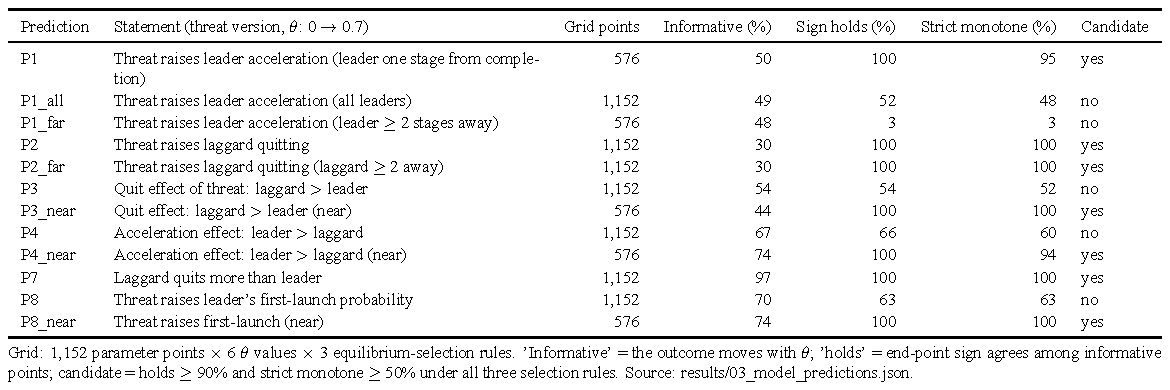
\includegraphics[max width=\textwidth,max height=0.85\textheight]{tables_tex/T_model_predictions.pdf}
\end{table}

\begin{figure}[htbp]
\centering
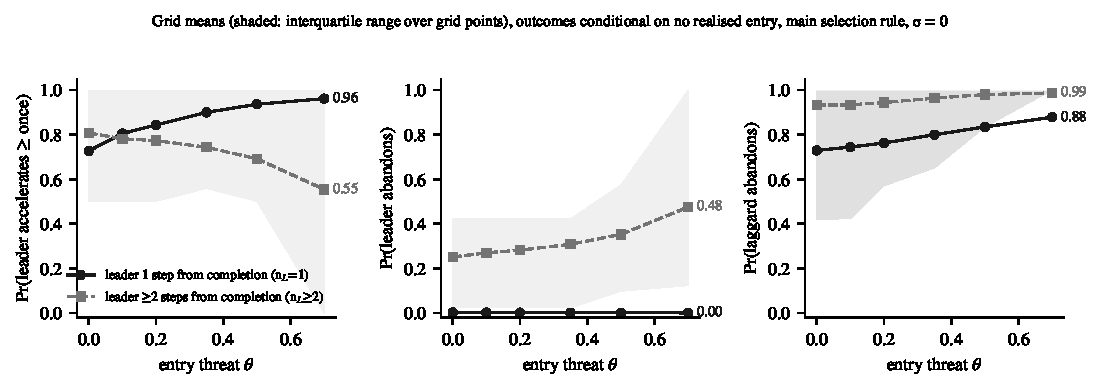
\includegraphics[width=\textwidth]{figures/fig_model_comparative_statics.pdf}
\caption{Grid means of the threat-conditional outcomes as $\theta$ rises (shaded: interquartile range over grid points; main selection rule; $\sigma = 0$). Left: probability that the leader accelerates at least once, for leaders one stage from completion and for leaders two or more stages away. Centre: probability that the leader abandons. Right: probability that the laggard abandons. Source: results/03\_grid\_outcomes.parquet via code/make\_figures.py.}
\label{fig:model}
\end{figure}

The escape response belongs to leaders one stage from completion: for them, threat raises acceleration at every informative point (end-point sign \ModelPOneHolds\%, strict monotonicity \ModelPOneStrict\%), whereas for leaders two or more stages away the sign holds at only \ModelPOneFarHolds\% of points and the typical response is less acceleration and more abandonment (the probability that such a leader abandons rises with $\theta$ at \ModelPTwoLFarThrUp\% of points). Being ahead of the rival is therefore not the condition for pre-emption; being close to completion is, which is the step-by-step logic of \citet{aghion2009entry} in a finite race. The second result concerns the laggard, whose abandonment rises with threat everywhere it moves (\ModelPTwoHolds\%) and who abandons more than the leader at every $\theta$ (\ModelPSevenHolds\%). The third is that the threat and the realisation of entry predict opposite things for the leader: in the unconditional version, which mixes realised entries in, the leader's acceleration falls with $\theta$ at \ModelPOneUncViolated\% of points and rises at only \ModelPOneUncHolds\%, because once the entrant has arrived the unfinished prizes are cut and speed no longer pays; the laggard's abandonment rises in both versions (unconditional violation \ModelPTwoUncViolated\%).

A fourth candidate did not survive. The survey block also asks whether `competitors' actions hard to predict' describes the firm's market, and I modelled this rival unpredictability $\sigma$ in two ways, as an implementation tremble that re-draws the realised effort level of an intended action and as a one-stage error in observing the rival's position. The two definitions give opposite dominant signs for the laggard's abandonment (tremble: \ModelPFiveTrembleDir{} at \ModelPFiveTrembleShare\% of informative points; observation noise: \ModelPFiveObsNoiseDir{} at \ModelPFiveObsNoiseShare\%), so no direction was registered and the item enters only as a control and in exploratory tests.

\subsection{Hypotheses}

The registered hypotheses translate the three grid results into the survey's variables, with the frontier group $g = 2$ standing for the leader one stage from completion and the laggard group $g = 0$ for the follower; the groups are defined from the R\&D-staff share in Section~\ref{sec:data}. Perceived entry threat should raise the probability that a frontier firm adopts lead-time protection (H1, the escape margin) and the probability that a laggard reports an abandoned or suspended activity (H2, the exit margin), the second also in the objective entry rate. The falsification rule for H2 is deliberately asymmetric, and its weakness should be stated: H2 counts as falsified only if both the perceived and the objective slope are non-positive, so a positive but imprecise slope cannot falsify it, and the label set therefore includes `directional' for that case. The two responses should be asymmetric in the directions the model gives: the abandonment slope should be larger for laggards than for frontier firms (H3) and the pre-emption slope larger for frontier firms than for laggards (H4). Laggards should abandon more than frontier firms whatever the level of threat (H5). And realised entry, measured by the industry entry rate, should not raise pre-emption among frontier firms (H6), tested as an equivalence hypothesis with a pre-set bound because a null result cannot otherwise be told from low power. The agents' predictions for the same six contrasts were frozen before the survey test (Table~\ref{tab:agentcontrasts}).

\section{Data and measurement}
\label{sec:data}

\subsection{The Korean Innovation Survey}

The Korean Innovation Survey is an officially approved national statistic (approval no.\ \KISApprovalNo) conducted under Article 18 of the Statistics Act, with responses protected under Articles 33 and 34 of the same Act; it has been carried out since \KISSinceYear{} by the Science and Technology Policy Institute (STEPI), follows the OECD Oslo Manual, and the four waves used here were fielded by Gallup Korea (statements printed on page 1 of each questionnaire). Manufacturing and services are surveyed in alternate years with sector-specific questionnaires, each covering a three-year reference period: the 2022 manufacturing wave (\NTwoZeroTwoTwoM{} firms), the 2023 services wave (\NTwoZeroTwoThreeS), the 2024 manufacturing wave (\NTwoZeroTwoFourM) and the 2025 services wave (\NTwoZeroTwoFiveS), together \NFirms{} firms; the 2020 manufacturing wave has no market-environment block and is excluded. The microdata are licensed research-use files provided by STEPI and cannot be redistributed; the code, the audited item maps and every result file are public (Data availability).

Every variable used here was read in both the codebook of the provision file and the printed questionnaire of its wave and transcribed with its printed response codes into an item map that the loader applies; the maps, with observed value distributions, are part of the registered package, Table~\ref{tab:variables} lists the items with their questionnaire wording, and \ref{app:items} records the three places where the reading changed the data (a shifted code scheme in the 2023 services file, two codebook descriptions copied from another question in the 2024 and 2025 files, and two undocumented values, a sentinel and an implausible founding year, treated as missing).

\begin{table}[htbp]
\centering
\caption{Survey items used, with verbatim questionnaire wording. Source: item\_maps/item\_map\_\textless wave\textgreater.json, generated by code/make\_tables.py.}
\label{tab:variables}
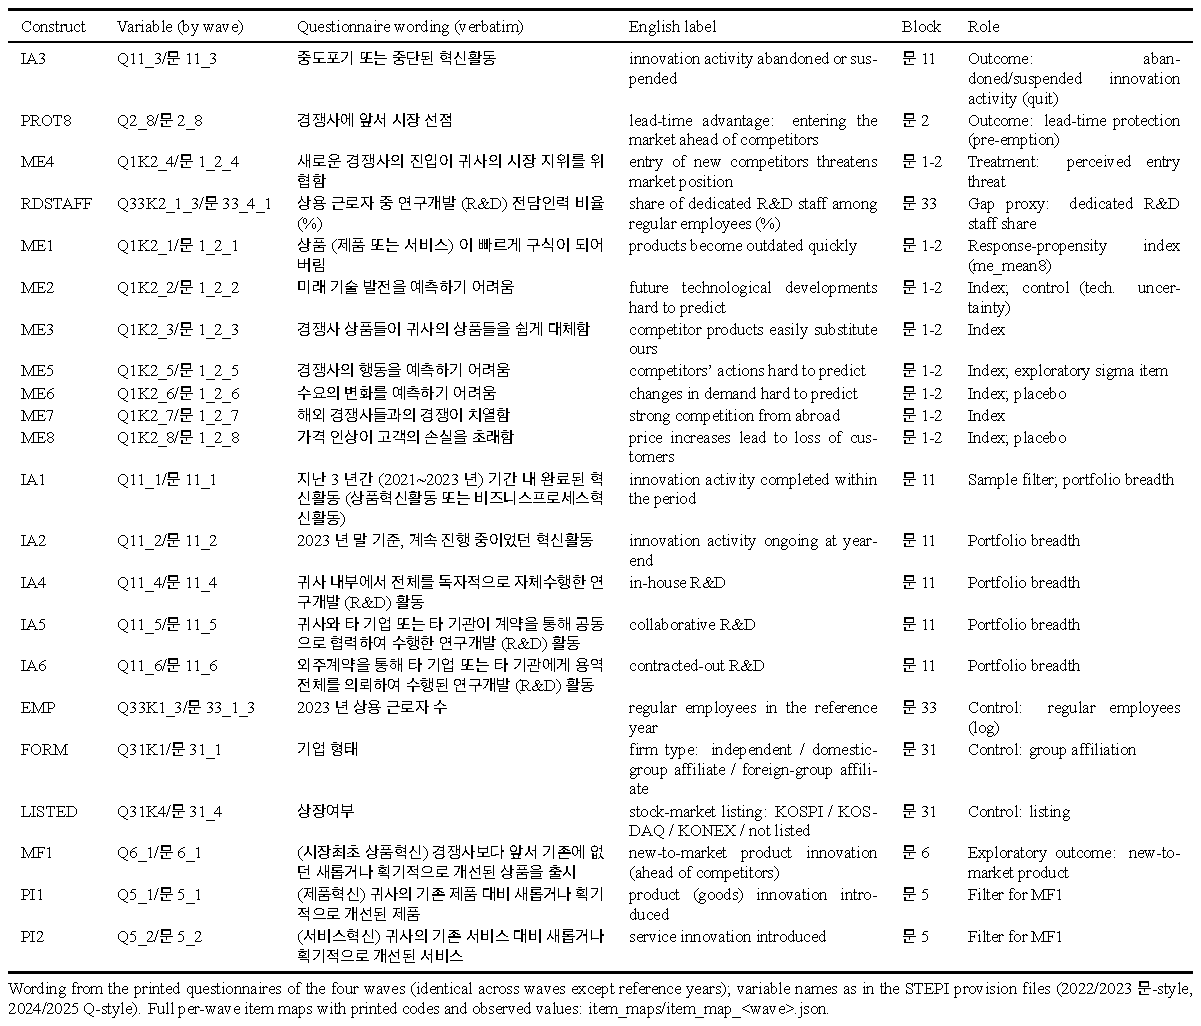
\includegraphics[max width=\textwidth,max height=0.85\textheight]{tables_tex/T_variables.pdf}
\end{table}

\subsection{Outcomes}

The exit margin is the item `innovation activity abandoned or suspended' in the block that asks which innovation activities the firm had during the reference period (block 11, item 3). It is answered by all firms but is meaningful only for firms with any innovation activity, so, as in \citet{garciavega2010determinants} and the CIS abandonment literature, the abandonment models are estimated on innovation-active firms (any `yes' among completed, ongoing, in-house R\&D, collaborative R\&D or contracted-out R\&D; \NQuitSample{} firms, \QuitEvents{} with an abandoned or suspended activity, \QuitRatePct\%). Two stricter variants are pre-registered robustness outcomes: abandonment without any completed activity (\ExitStrictRatePct\% of innovation-active firms) and abandonment with neither a completed nor an ongoing activity (\ExitFullRatePct\%). The escape margin is the item `lead-time advantage: entering the market ahead of competitors' in the block on methods used to protect innovations (block 2, item 8), answered by all firms (\PreemptEvents{} of \NFirms{}, \PreemptRatePct\%). New-to-market product innovation (block 6, item 1), the model's `finishing first', is asked only of product innovators and is used in an exploratory, selection-corrected test on the manufacturing waves because the services base rates are too low to carry a test. Table~\ref{tab:base} gives the rates by wave; abandonment is far more common in the 2022 manufacturing wave (\QuitRateTwoZeroTwoTwoMPct\%) than in any later wave (\QuitRateTwoZeroTwoThreeSPct\% to \QuitRateTwoZeroTwoFourMPct\%), and lead-time protection is a manufacturing practice (\PreemptRateTwoZeroTwoTwoMPct\% and \PreemptRateTwoZeroTwoFourMPct\% against \PreemptRateTwoZeroTwoThreeSPct\% and \PreemptRateTwoZeroTwoFiveSPct\% in services), two differences that the sector split below has to respect.

\begin{table}[htbp]
\centering
\caption{Outcome base rates by wave. Source: results/02\_marginals.json, generated by code/make\_tables.py.}
\label{tab:base}
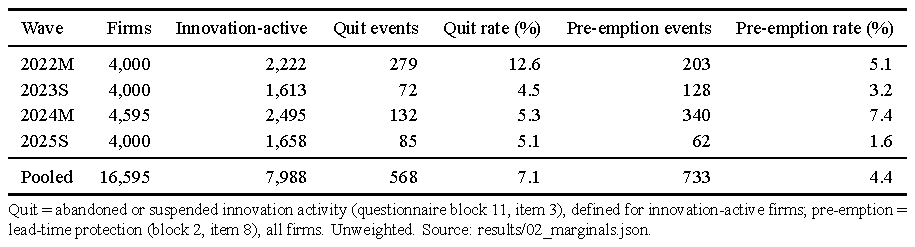
\includegraphics[max width=\textwidth]{tables_tex/T_base_rates.pdf}
\end{table}

\subsection{Perceived entry threat and its adjustment}

The treatment is the item `entry of new competitors threatens market position', rated from 0 (`not applicable') to 5 (`very high') for the reference period, in a block of eight statements about the firm's market environment that reproduces the Eurostat CIS 2020 block item for item (the Korean wording was compared with the Eurostat questionnaire, saved with the project). The block has served as a source of treatment variables before: \citet{woerter2019competitive} relate its obsolescence and technological-uncertainty items to green R\&D in Austrian, German and Swiss firms, and \citet{peneder2014competition} recover the inverted-U between competition and innovation from it in Swiss firm data. A firm's rating of this statement is not independent of how it rates the others: of the \MEPairsTotal{} pairs of items in the block, \MEPairsGeHalf{} correlate at 0.5 or above, and the entry-threat item itself correlates \CorrThreatPlacebo{} with `changes in demand hard to predict' and \CorrThreatSigma{} with `competitors' actions hard to predict', so part of each rating is the respondent's general propensity to rate pressures high. The registered treatment is the within-wave residual of the entry-threat item from a regression on the other seven items of the block, entered separately, as built by the registered loader; it is not re-standardised, and its standard deviation is \ThreatResidSDPooled{} in the pooled sample (\ThreatResidSDTwoZeroTwoTwoM{} to \ThreatResidSDTwoZeroTwoFourM{} by wave), so the slopes below are per unit of the residual and read as per-standard-deviation slopes to within one per cent. The registration text describes the same variable as the residual on the eight-item mean, standardised; the code whose hash the registration records is the one that ran (\ref{app:deviations} records the discrepancy), and because the eight-item mean contains the treatment item and would have removed part of its variance, Section~\ref{sec:results} reports that recipe and a leave-one-out variant as exploratory rows. The raw 0--5 item is a pre-registered robustness specification, and the eight-item mean enters every model as a control. The two items with no counterpart in the model, demand unpredictability and `price increases lead to loss of customers', are the pre-registered placebos, residualised within wave on the eight-item mean and standardised, which is the registration text's recipe.

\subsection{The technology gap}

The model's state variable is distance to completion, which no survey measures. The pre-registered proxy is the share of dedicated R\&D staff among regular employees (block 33), reported by all firms, ranked within industry (two-digit KSIC division) and wave. A staff share measures how formally a firm organises R\&D, not how far a particular project has progressed, and firms without dedicated R\&D staff do innovate: \SecGapNInnovManuZero{} manufacturing and \SecGapNInnovServZero{} services firms in that group report an innovation activity in the activity block, through completed or ongoing activities, collaborative R\&D or R\&D contracted out. The proxy separates firms with a standing capacity to finish a technical project from firms without one, and in the model it is the firm able to finish within the horizon that has something to protect by hurrying. Because \ShareZeroRDManuMinPct--\ShareZeroRDManuMaxPct\% of manufacturing firms and \ShareZeroRDServMinPct--\ShareZeroRDServMaxPct\% of services firms report no dedicated R\&D staff at all, terciles degenerate; the registered grouping is instead $g = 0$ for firms with no dedicated R\&D staff (\GapZeroN{} firms), $g = 1$ for firms with a positive share at or below the median of positive shares in their industry-wave cell (\GapOneN), and $g = 2$ for firms above that median (\GapTwoN), borrowing the section-wave or wave median where a cell has fewer than ten positive values and recording which median was used. Group 2 is the survey counterpart of the leader one stage from completion and group 0 of the follower; the correspondence is a proxy, and its limits are weighed against the results in Section~\ref{sec:discussion}. An exploratory alternative, R\&D expenditure over sales in the same three-way grouping (available only for innovation-active firms), is reported with the robustness checks.

\subsection{Realised entry: industry entry rates}

Realised entry is measured by the enterprise birth rate of the firm's two-digit industry from the Business Demography Statistics (KOSIS table DT\_6BD1101, national rows), in which active enterprises in a year are those with annual sales or regular workers during that year, birth enterprises are those newly recorded, and the birth rate is births over active enterprises times one hundred. For each firm the rate is averaged over the three reference years of its wave, so no year after the survey's reference period enters; every one of the \NFirms{} firms has a value (\EntryRateMissingFirms{} missing). Across industry cells the rate ranges from \EntryRateMinTwoZeroTwoFourMPct\% in division \EntryMinIndTwoZeroTwoFourM{} (\EntryMinIndTwoZeroTwoFourMLabel) to \EntryRateMaxTwoZeroTwoFourMPct\% in division \EntryMaxIndTwoZeroTwoFourM{} (\EntryMaxIndTwoZeroTwoFourMLabel) in the 2024 manufacturing wave, and from \EntryRateMinTwoZeroTwoFiveSPct\% in division \EntryMinIndTwoZeroTwoFiveS{} (\EntryMinIndTwoZeroTwoFiveSLabel) to \EntryRateMaxTwoZeroTwoFiveSPct\% in division \EntryMaxIndTwoZeroTwoFiveS{} (\EntryMaxIndTwoZeroTwoFiveSLabel) in the 2025 services wave; in the 2022 manufacturing wave the extremes are \EntryMinIndTwoZeroTwoTwoMLabel{} (\EntryMinIndTwoZeroTwoTwoMPct\%) and \EntryMaxIndTwoZeroTwoTwoMLabel{} (\EntryMaxIndTwoZeroTwoTwoMPct\%). The rate is standardised within the pooled sample before use. The research plan also called for Chinese import penetration by industry in the manner of \citet{bloom2016trade}, whose effects on innovation differ by setting (more patenting and IT in European firms exposed to Chinese imports, less patenting in US sectors, a shift from process to product innovation and more exit among differentiated Canadian firms; \citealp{bloom2016trade,autor2020foreign,kueng2016emerging}); the Korean trade-by-enterprise statistics classify imports by the importing firm's industry in seven manufacturing groups, which mixes intermediate inputs with competing goods and does not reach the two-digit level, and building a product-to-industry concordance from scratch would have introduced an unverified mapping. The indicator was dropped before registration and the foreign-competition item of the market-environment block serves only as a control.

\subsection{Controls and samples}

Following the practice of innovation-survey econometrics \citep{mairesse2010using}, all models include industry (two-digit) and wave fixed effects, the logarithm of regular employees, the logarithm of one plus firm age (reference year minus founding year, from the register fields of the provision file), indicators for affiliation with a domestic or a foreign business group, a listing indicator and the response-propensity index; the abandonment models add portfolio breadth, the count of the other innovation-activity items answered `yes', because firms that run more projects abandon more of them \citep{klingebiel2021optionality}. Listwise deletion on the controls removes one firm from each sample (\NPreemptModel{} and \NQuitModel{} observations). Clusters are industry-by-wave cells, \NClusters{} in the pre-emption models and \NClustersQuit{} in the abandonment models. Sampling weights are available in all waves and are a pre-registered robustness specification; the main estimand is the unweighted within-sample association.

\section{Pre-registration and the agent experiments}
\label{sec:prereg}

\subsection{What was registered, and when}

The study was registered on the Open Science Framework on \OSFRegisteredKST{} KST (\ifanon the registration and project links are given on the title page for the editor; an anonymised view-only copy of the registered documents and the reproduction package is at \url{\OSFReviewCopyURL}\else registration \url{\OSFRegistrationURL}; project \url{\OSFProjectURL}\fi), after the survey files had been read, mapped and merged and before any statistic combining an outcome with a treatment had been computed. It contains the six hypotheses with their model basis and falsification conditions, the variable definitions generated from the item maps, the analysis script and its SHA-256 hash, the frozen agent predictions (Table~\ref{tab:agentcontrasts}) and an embargo log, which matters because secondary-data registrations are only as credible as the evidence that the data were not looked at first \citep{weston2019recommendations}: the loader refuses any cross-tabulation of outcome and treatment columns, and the analysis script refuses to run on real outcomes without a registration record (\ref{app:deviations} lists what was computed before registration). A power analysis on synthetic outcomes drawn at the observed base rates gave minimum detectable interaction slopes at 80\% power of \MDEQuitPp{} percentage points for abandonment and \MDEPreemptPp{} for pre-emption.

The decision rules were fixed in the script. Tests of H1--H5 are one-sided at 5\% with Holm adjustment across the five \citep{holm1979simple}; a hypothesis is `supported' if the point estimate has the predicted sign and the Holm-adjusted $p$-value is below 0.05, `directional' if the sign is right but the adjusted $p$-value is not, and `not supported' otherwise. H6 is an equivalence test: `equivalence' if the 90\% interval of the entry-rate slope among frontier firms lies inside $\pm$\KISHSixDelta{} (the pre-emption minimum detectable effect), `positive effect' or `negative effect' if it lies entirely outside the band on one side, and `inconclusive' otherwise. Primary inference is the wild cluster bootstrap-$t$ with Rademacher weights, \NBoot{} draws, industry-by-wave clusters and percentile-$t$ intervals; the cluster-robust $t$ is reported as secondary because in a permutation control run before registration it over-rejected for regressors that vary only at the cluster level \citep{cameron2008bootstrap}; the rejection rates are in \ref{app:deviations}. A known-answer run with planted slopes recovered them and returned zero for the planted placebos.

\subsection{The agent experiments}
\label{sec:agents}

Language models prompted with a role reproduce much of the behaviour of human subjects in classic economic experiments \citep{horton2023large,chen2023emergence,argyle2023out}, play self-interested repeated games well and coordination games poorly \citep{akata2025playing}, and have been used to generate and test hypotheses on simulated subjects \citep{manning2024automated}; surveys catalogue the promise and alignment problems \citep{gao2024large,park2023generative}. An LLM is not a firm, and the agents were handed the model's environment, prizes and equilibrium-playing rival, so their independence from the theorist is one of derivation, not setting; what they supply is a second prediction generator whose reasoning is written down.

Two frontier models, Claude fable-5 (Anthropic; Bedrock model identifier \ModelIdFable, region \ModelRegionFable) and GPT-5.6 (OpenAI; \ModelIdGpt{} through the Bedrock Mantle interface, region \ModelRegionGpt), were called without a system prompt at default sampling as a Korean executive deciding about a product-development project, in Korean and, as a paraphrase check, in English (Stage A calls on \StageACallsDate{}, Stage B calls on \StageBCallsDate{}; times in \ref{app:protocol}). Each persona was drawn from a KIS record using four treatment-free register attributes (two-digit industry, employee-size band, firm age and group affiliation), coarsened in the public logs (\ref{app:disclosure}). Every template was checked against a forbidden list of theory terms (\ref{app:vocabulary}), which keeps the hypothesis, not the structure of the problem, out of the prompt; and the options were shown in a logged random order, because a content-free probe had shown both models to favour the first option (\ref{app:protocol}).

The environment is the three-period race of Section~\ref{sec:theory} in money units (\ref{app:calibration} states every constant), so the agents play the model itself against a rival that follows the solved model's equilibrium policy at the true state; twelve cells cross three positions (one stage behind, level, one stage ahead) with the entry threat and a one-stage observation noise. One parameter was calibrated by a rule fixed before the scan was read: the draft acceleration cost of \EnvDraftAccelCostBn{} billion won put the model's own frontier leader at an acceleration probability of \EnvDraftLeaderAccelNoThreat{} without any threat, a ceiling no agent could have moved, so the cost was scanned on a 0.5-billion-won grid for the smallest value at which the model's leader and laggard responses were neither at a ceiling nor flat, \EnvAccelCostBn{} billion won (Table~\ref{tab:env}). The vignette is the third version written; the two discarded versions each produced an artefact, diagnosed before it was believed (\ref{app:design}).

Stage A is a one-shot decision: the persona reads the rules and the current situation and returns one of continue, accelerate or stop with a two-sentence reason in JSON. The \StageAPersonas{} personas times twelve cells, two languages and two models gave \StageACalls{} calls, of which \StageAParseFail{} returned no parseable JSON and is kept as missing. The placebo attribute and the option-position effect form one null family per stage, tested within cells by re-randomisation with Holm adjustment across arms; the smallest adjusted $p$-value is \StageAPlaceboMinHolm{} in Stage A and \StageBPlaceboMinHolm{} in Stage B, so the pre-set kill test did not fire.

Stage B is the three-period race: \StageBPersonas{} of the personas play each of the twelve cells against the equilibrium rival, receiving each period the rules, history and state but never the rival's action. Of \StageBEpisodes{} episodes, \StageBComplete{} completed and \StageBParseFailed{} ended unparsed, all in the Claude--Korean arm through a provider-side refusal that was diagnosed and replayed (\ref{app:refusal}); the residue is kept as missing. Because environment draws are seeded by episode index, shared by the two models within a language, the two arms of a language are not independent replications of the placebo check; the runner itself was validated with a scripted equilibrium agent (\ref{app:protocol}).

A contrast is called `+' if its 95\% persona-bootstrap interval lies above zero, `$-$' if below and `0' otherwise, and the four-arm consensus requires three to agree. The agents overshot the model before agreeing with it: in Stage A the threat raised the frontier firm's acceleration by \SAHOneMin{} to \SAHOneMax{}, against \ModelPOneLeaderAccelThreat{} in the model's own period-one policy for the same seat (Table~\ref{tab:stagea}), and the laggard's stopping by \SAHTwoMin{} to \SAHTwoMax{} against the model's \ModelPOneLaggardQuitThreat. In sign, all four arms predicted every one of H1 to H5 (Table~\ref{tab:agentcontrasts}, Figure~\ref{fig:agents}). In the race the magnitudes were closer to the model and the agents reproduced its distinction between threat and realised entry: conditional on no entry the frontier firm's acceleration rose with the threat in three of four arms (\SBHOneMin{} to \SBHOneMax); unconditionally the contrast ranged from \SBHOneUncondMin{} to \SBHOneUncondMax{} and the H6 consensus was `0' (Table~\ref{tab:stageb}). The frozen table therefore read theory `+', agents `+' for every hypothesis except H6 (theory `not +', agents `0'); the two models differed only in how readily they stopped (\ref{app:agentshares}).

\begin{table}[htbp]
\centering
\caption{Model outcomes for the agent's seat in each cell of the calibrated environment. Source: results/05\_agent\_stage\_b.json (model\_predictions), generated by code/make\_tables.py.}
\label{tab:env}
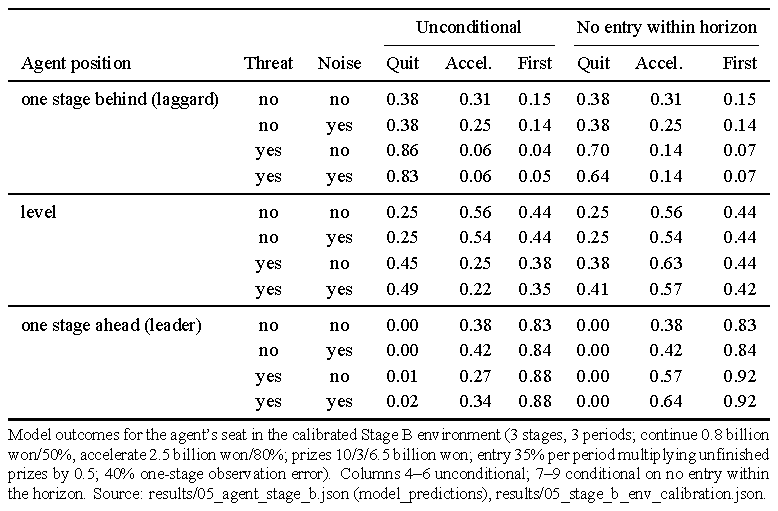
\includegraphics[max width=\textwidth]{tables_tex/T_environment.pdf}
\end{table}

\begin{table}[htbp]
\centering
\caption{Frozen agent predictions for the six hypotheses: contrasts of cell shares with persona-bootstrap intervals and sign calls, by stage and arm. Source: prereg/agent\_predictions\_v1.json (SHA-256 \PredSha\ldots), generated by code/make\_tables.py.}
\label{tab:agentcontrasts}
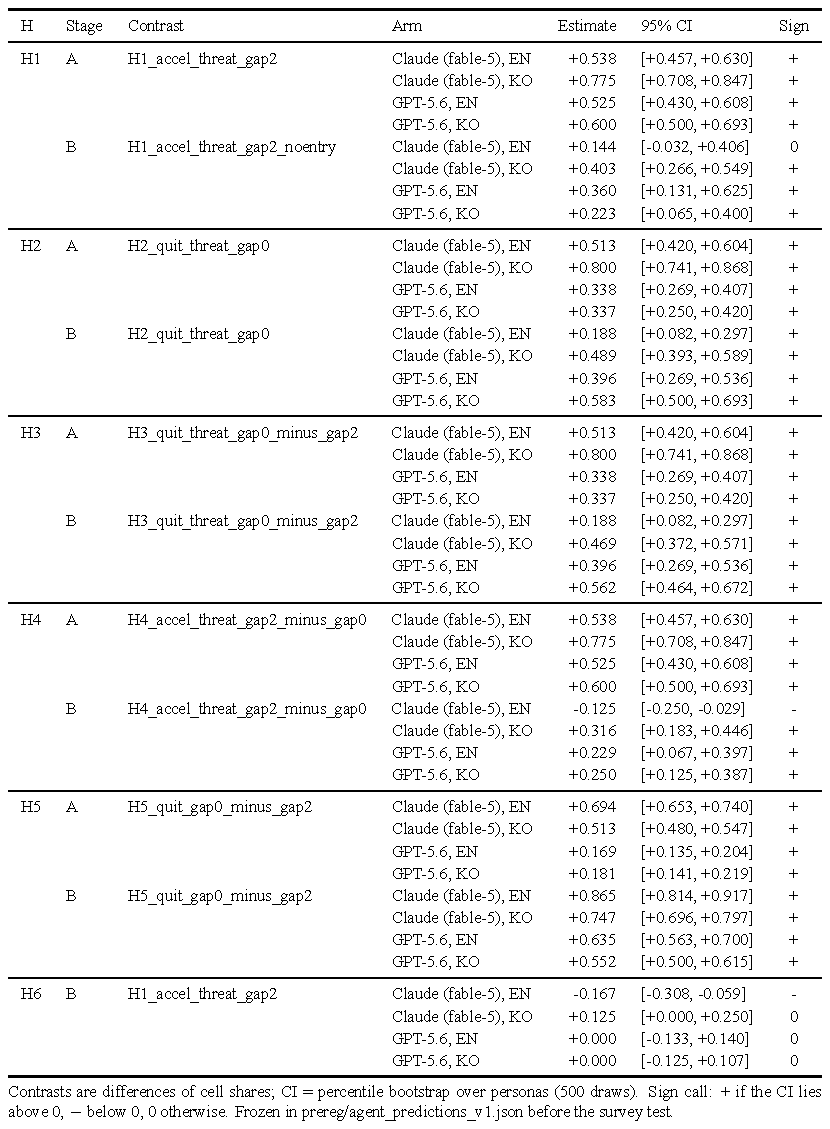
\includegraphics[max width=\textwidth,max height=0.88\textheight]{tables_tex/T_agent_contrasts.pdf}
\end{table}

\begin{table}[htbp]
\centering
\caption{Stage A cell shares: one-shot period-1 decisions by position, threat and noise, for each arm. Source: results/04\_agent\_stage\_a.json, generated by code/make\_tables.py.}
\label{tab:stagea}
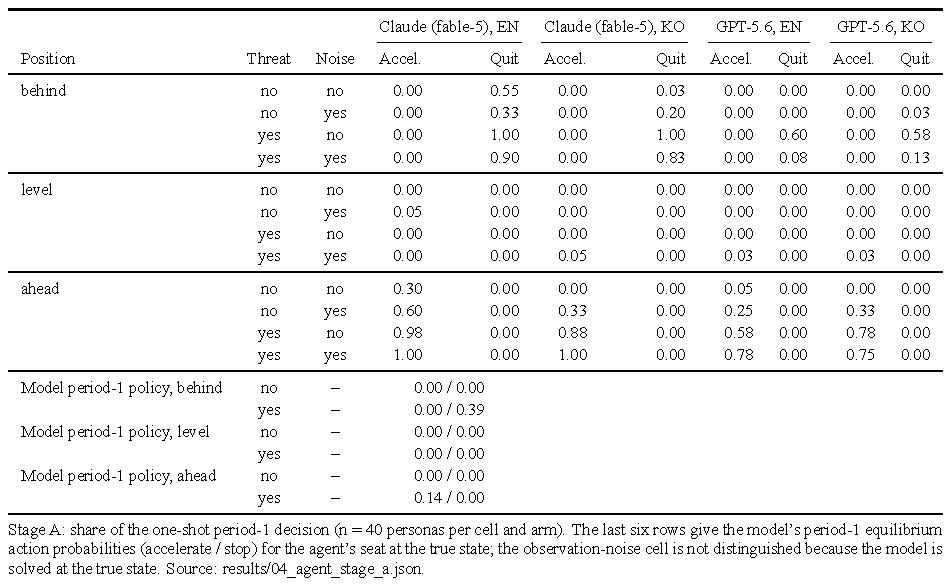
\includegraphics[max width=\textwidth]{tables_tex/T_stageA_cells.pdf}
\end{table}

\begin{table}[htbp]
\centering
\caption{Stage B cell shares: episodes in which the agent accelerated at least once or stopped, by position, threat and noise, for each arm. Source: results/05\_agent\_stage\_b.json, generated by code/make\_tables.py.}
\label{tab:stageb}
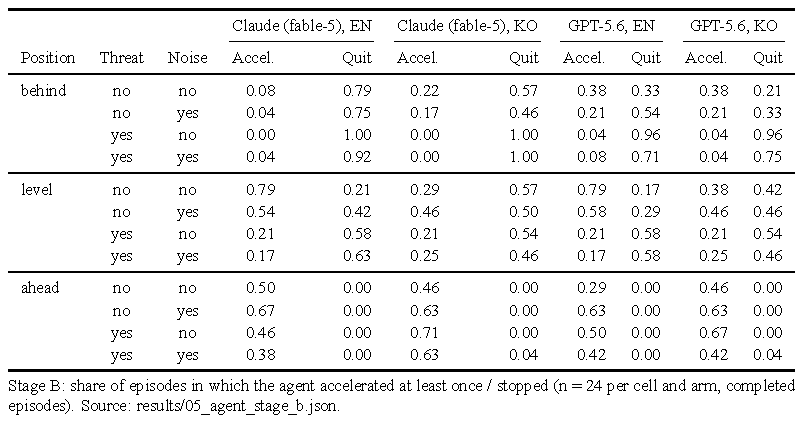
\includegraphics[max width=\textwidth]{tables_tex/T_stageB_cells.pdf}
\end{table}

\begin{figure}[htbp]
\centering
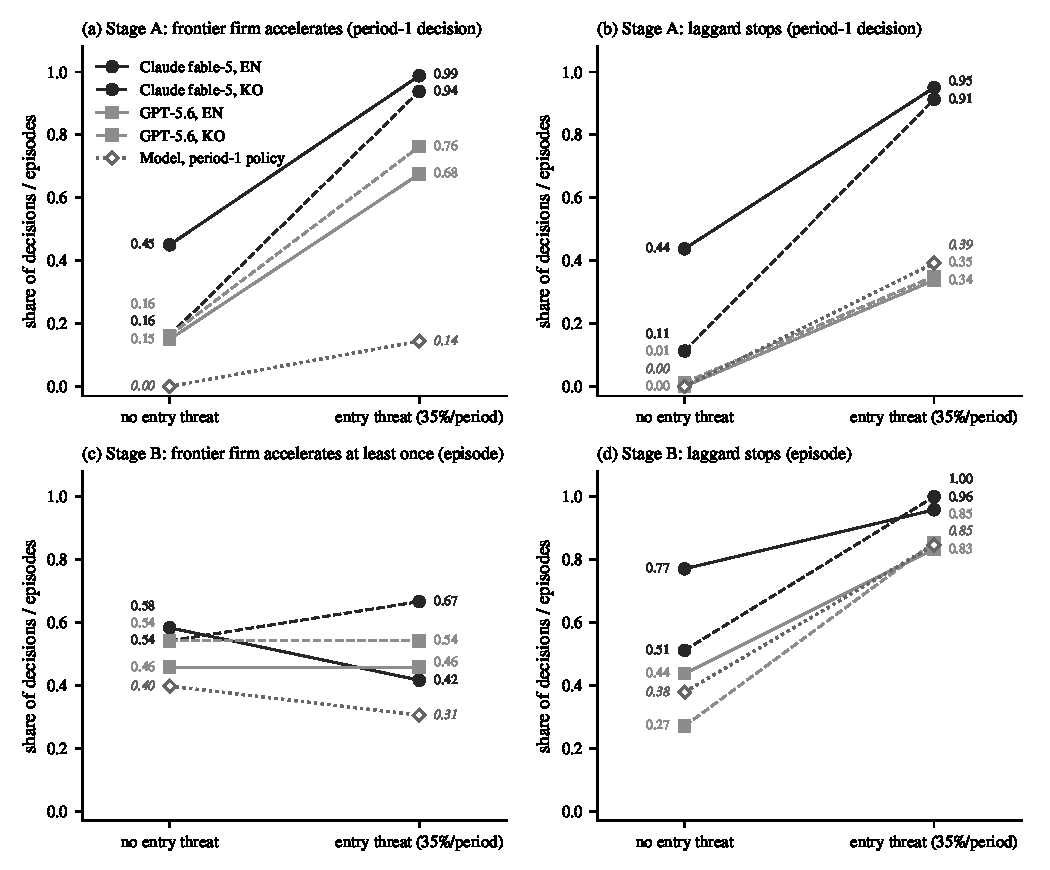
\includegraphics[width=\textwidth]{figures/fig_agents.pdf}
\caption{Agent choices and the model's prediction in the two hypothesis cells. (a), (b): Stage A period-1 shares of accelerating (frontier firm) and stopping (laggard) without and with entry threat, by arm, with the model's period-1 equilibrium policy. (c), (d): Stage B episode shares. Sources: results/04\_agent\_stage\_a.json, results/05\_agent\_stage\_b.json via code/make\_figures.py.}
\label{fig:agents}
\end{figure}

\section{Results}
\label{sec:results}

\subsection{The pre-registered tests}

The six confirmatory tests (Table~\ref{tab:main}, Figure~\ref{fig:coef}; full coefficient vectors in Table~\ref{tab:coef}) share one estimating equation,
\begin{equation}
y_{i} = \sum_{g \in \{0,1,2\}} \left[ a_{g}\, \mathbf{1}(G_i = g) + b_{g}\, x_{i}\, \mathbf{1}(G_i = g) \right] + \mathbf{z}_{i}'\boldsymbol{c} + \mu_{j(i)} + \tau_{w(i)} + \varepsilon_{i},
\label{eq:main}
\end{equation}
a linear probability model in which $y_i$ is the outcome of firm $i$, $G_i$ its gap group, $x_i$ the treatment (the perceived-threat residual of Section~\ref{sec:data} for H1--H5; the standardised industry entry rate for H6 and the objective half of H2), $\mathbf{z}_i$ the controls, and $\mu_j$ and $\tau_w$ industry and wave fixed effects. The treatment is centred, so $a_g$ is the group's adjusted mean at average threat. H1 is $b_2 > 0$ in the pre-emption model, H2 $b_0 > 0$ in the abandonment model, H3 $b_0 - b_2 > 0$ there, H4 $b_2 - b_0 > 0$ in the pre-emption model, H5 $a_0 - a_2 > 0$ in the abandonment model, and H6 the equivalence test on $b_2$ in the pre-emption model with the entry rate as $x$. As in \citet{garciavega2010determinants}, abandonment is the CIS item among innovation-active firms with industry controls; added are the market-environment treatment, the gap interaction and the second margin. Identification is cross-sectional: the perceived-threat slopes compare firms in the same industry and wave who rate the entry threat differently, net of their general propensity to rate pressures high, so the estimates are associations, and I write them as such. The entry-rate slopes vary only across industry-wave cells, so the wild bootstrap carries the inference and industry-by-wave fixed effects, which absorb the rate's own variation and leave only its interaction with the gap, are the decisive robustness check for the objective hypotheses.

\begin{table}[htbp]
\centering
\caption{Pre-registered confirmatory tests. Estimates are changes in outcome probability per one standard deviation of the treatment within the gap group (H5: difference of group intercepts at average threat); wild cluster bootstrap-$t$ inference with industry-by-wave clusters; decisions by the registered rule. Source: results/06\_kis\_main.json, generated by code/make\_tables.py.}
\label{tab:main}
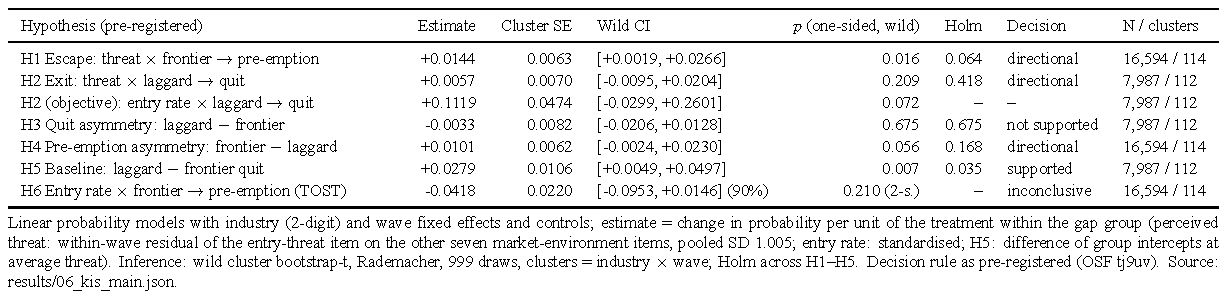
\includegraphics[max width=\textwidth]{tables_tex/T_kis_main.pdf}
\end{table}

\begin{figure}[htbp]
\centering
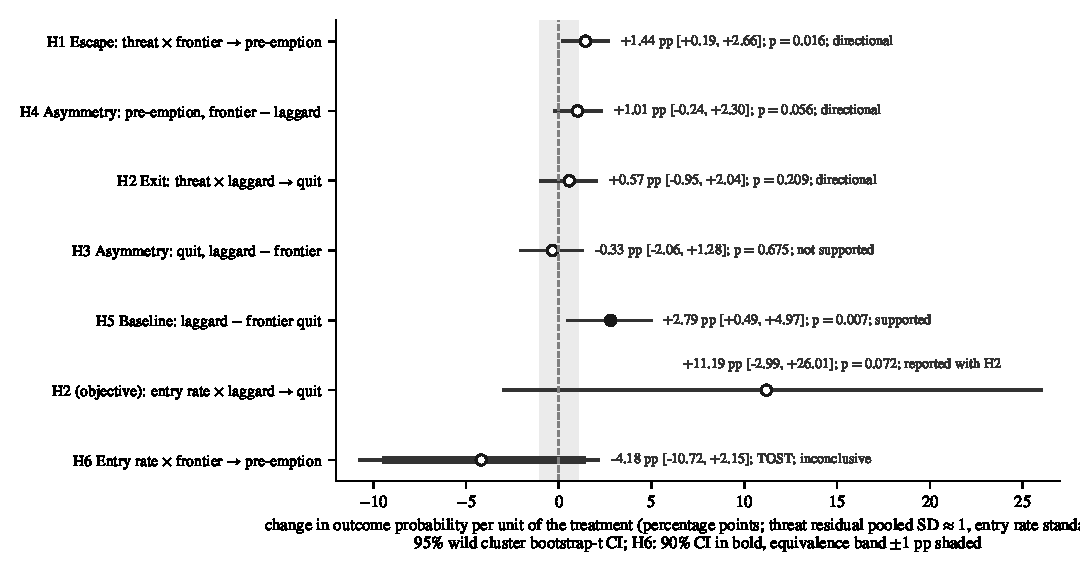
\includegraphics[width=\textwidth]{figures/fig_kis_coefficients.pdf}
\caption{Confirmatory estimates in percentage points with 95\% wild cluster bootstrap-$t$ intervals (H6: 90\% interval in bold, equivalence band $\pm$\KISHSixDeltaPp{} percentage points shaded). Source: results/06\_kis\_main.json via code/make\_figures.py.}
\label{fig:coef}
\end{figure}

\begin{table}[htbp]
\centering
\caption{Full coefficient vectors of the four main models, with cluster-robust standard errors. Source: results/06\_kis\_main.json, generated by code/make\_tables.py.}
\label{tab:coef}
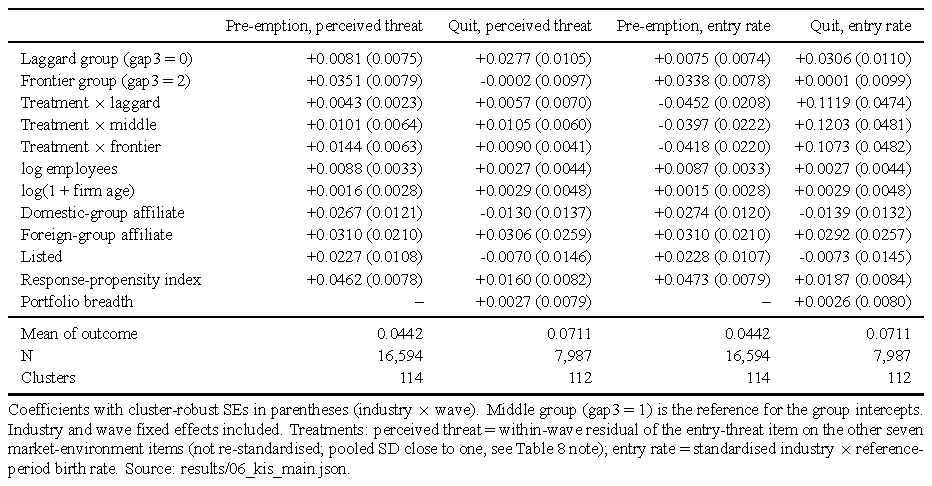
\includegraphics[max width=\textwidth]{tables_tex/T_kis_coefficients.pdf}
\end{table}

On the escape margin, one unit of the perceived-threat residual is associated among frontier firms with \KISHOnePp{} percentage points more lead-time protection (cluster SE \KISHOneSE{} in probability units; wild 95\% interval \KISHOneLoPp{} to \KISHOneHiPp{} percentage points; one-sided wild $p$ = \KISHOnePOne, cluster-robust $t$ $p$ = \KISHOnePOneT), about \KISHOneRelMeanPct\% of the sample mean of \PreemptRatePct\% and \KISHOneRelFrontierPct\% of the frontier group's own rate of \RawPreGTwoPct\%. The unadjusted interval excludes zero, and \RobHOneDistinctSigCount{} of the \RobHOneDistinctSpecCount{} distinct pre-registered robustness specifications agree in sign with one-sided $p$ at or below \RobHOneDistinctMaxSigP{} (Table~\ref{tab:robust}; the two quit-definition rows repeat the pre-emption model and are not counted), which would ordinarily be read as support; under the registered Holm rule across five tests the adjusted $p$-value is \KISHOneHolm{} and the label is `directional', and I keep it. The pre-emption slope is positive in all three groups (\CoefPreXGZero, \CoefPreXGOne{} and \CoefPreXGTwo{} for laggards, the middle group and frontier firms) and rises with the gap group; the frontier--laggard difference, H4, is \KISHFourPp{} percentage points (interval \KISHFourLoPp{} to \KISHFourHiPp; $p$ = \KISHFourPOne; Holm \KISHFourHolm; `directional'), and logit average marginal effects (\AMEPreXGZero, \AMEPreXGOne, \AMEPreXGTwo) order the groups the same way. At average threat the frontier group adopts lead-time protection far more often than the middle group (\CoefPreGTwo) and laggards slightly more (\CoefPreGZero), and the response-propensity index is strongly positive (\CoefPreMeMeanEight): firms that rate every pressure high also report more protection methods, the reason the index is removed from the treatment and held fixed.

On the exit margin there is no comparable movement. Among laggards the abandonment slope is \KISHTwoPp{} percentage points per standard deviation (interval \KISHTwoLoPp{} to \KISHTwoHiPp; $p$ = \KISHTwoPOne; Holm \KISHTwoHolm), a point estimate below the registered minimum detectable effect of \MDEQuitPp{} percentage points, with an interval that includes zero and effects of that size, which is why the label is `directional', not `not supported'; the design compares groups within a margin, never one margin against another, so H1 and H2 carry the same label. The other two groups' slopes are as large or larger (\CoefQuitXGOne{} for the middle group, \CoefQuitXGTwo{} for frontier firms), so the laggard--frontier difference of H3 has the wrong sign (\KISHThreePp{} percentage points; interval \KISHThreeLoPp{} to \KISHThreeHiPp; $p$ = \KISHThreePOne) and H3 is `not supported'. Laggards do abandon more at every level of threat: their adjusted mean exceeds the frontier group's by \KISHFivePp{} percentage points (interval \KISHFiveLoPp{} to \KISHFiveHiPp; $p$ = \KISHFivePOne; Holm \KISHFiveHolm), about \KISHFiveRelMeanPct\% of the sample abandonment rate, and H5 is `supported'. The frontier group's intercept is indistinguishable from the middle group's (\CoefQuitGTwo), so the baseline difference separates firms with no dedicated R\&D staff from everyone else. The unadjusted pooled rates run the other way (\RawQuitGZeroPct\%, \RawQuitGOnePct\% and \RawQuitGTwoPct\% for the three groups) because the laggard group is dominated by the services waves, where abandonment is rare; within industry and wave the difference is positive in both sectors (\RobManuHFiveEst{} in manufacturing, \RobServHFiveEst{} in services). Among controls, domestic-group affiliates and listed firms abandon slightly less often (\CoefQuitGroupDom{} and \CoefQuitListed, each within one standard error of zero; \CoefQuitObjGroupDom{} and \CoefQuitObjListed{} in the entry-rate models), foreign-group affiliates more, imprecisely (\CoefQuitGroupFor, SE \SEQuitGroupFor), and portfolio breadth adds little among innovation-active firms (\CoefQuitPortfolioBreadth).

The industry entry rate interacted with the laggard indicator gives \KISHTwoObjPp{} percentage points for one standard deviation of the rate (interval \KISHTwoObjLoPp{} to \KISHTwoObjHiPp; one-sided wild $p$ = \KISHTwoObjPOne; cluster-robust $t$ $p$ = \KISHTwoObjPOneT, the over-rejecting statistic), and because the perceived slope is also positive the falsification condition for H2, both slopes non-positive, is not met. But the slope is not laggard-specific (\CoefQuitObjXGZero, \CoefQuitObjXGOne{} and \CoefQuitObjXGTwo{} for the three groups), and with industry-by-wave fixed effects, which leave only the interaction, it falls to \RobFEIWHTwoObjEst. Firms in industries with more births abandon more in every gap group alike, a between-industry association (the industries at the top of the birth-rate range, \EntryMaxIndTwoZeroTwoTwoMLabel{} and \EntryMaxIndTwoZeroTwoFourMLabel{} in manufacturing, \EntryMaxIndTwoZeroTwoThreeSLabel{} and \EntryMaxIndTwoZeroTwoFiveSLabel{} in services, plausibly have low entry costs and short product lives, so projects are started and dropped freely) rather than a laggard's response to a particular entrant.

H6, realised entry and pre-emption, is the hypothesis the model made in the negative. The entry-rate slope among frontier firms is \KISHSixPp{} percentage points per standard deviation (90\% interval \KISHSixNinetyLoPp{} to \KISHSixNinetyHiPp), negative as the unconditional model predicts (agents' consensus `0', one arm negative), but the interval is too wide for the equivalence band of $\pm$\KISHSixDeltaPp{} percentage points and the registered verdict is `inconclusive'. The slope is negative in all three groups (\CoefPreObjXGZero, \CoefPreObjXGOne, \CoefPreObjXGTwo) and is \RobFEIWHSixEst{} with industry-by-wave fixed effects; the evidence is consistent with realised entry not raising pre-emption but cannot establish that it leaves it unchanged.

\subsection{Robustness}

Under the eight pre-registered alternative specifications (Table~\ref{tab:robust}; none was used for the decisions) the escape association survives the raw 0--5 threat item, industry-by-wave fixed effects, sampling weights and the exclusion of the 2023 services wave, with one-sided $p$-values at or below \RobHOneDistinctMaxSigP{} in \RobHOneDistinctSigCount{} of the \RobHOneDistinctSpecCount{} specifications that change the pre-emption model; the two stricter abandonment definitions leave that model untouched. The exception is the services-only sample: \RobServHOneEst{} ($p$ = \RobServHOneP) against \RobManuHOneEst{} ($p$ = \RobManuHOneP) in manufacturing. Lead-time protection is rare in services and most services firms have no dedicated R\&D staff (Section~\ref{sec:data}), so the services frontier group holds \SecGapNServTwo{} firms with \SecGapPreEventsServTwo{} lead-time events (\SecGapPreRateServTwoPct\%), against \SecGapNManuTwo{} firms and \SecGapPreEventsManuTwo{} events (\SecGapPreRateManuTwoPct\%) in manufacturing; a slope on \SecGapPreEventsServTwo{} events is not a test of the hypothesis. My reading is that the practice the item records exists in manufacturing and barely in services. The exit-margin null is stable across all \RobSpecCount: the laggard abandonment slope is positive in \RobHTwoPosCount{} and negative in \RobHTwoNegCount, its smallest one-sided $p$-value is \RobHTwoMinP, and the asymmetry H3 is negative in \RobHThreeNegCount. H5 is positive in \RobHFivePosCount{} specifications (below 0.05 in \RobHFiveSigCount) but falls to \RobStrictHFiveEst{} under the strict abandonment definition and \RobFullHFiveEst{} under the full one, so laggards more often report an abandoned or suspended activity alongside others, not the abandonment of everything they started.

\begin{table}[htbp]
\centering
\caption{Pre-registered robustness specifications and one exploratory row (gap proxy = R\&D expenditure over sales). Estimate and one-sided wild bootstrap $p$-value; \RobNBoot{} draws for robustness rows. Sources: results/06\_kis\_main.json, results/07b\_robustness\_gap\_proxy.json, generated by code/make\_tables.py.}
\label{tab:robust}
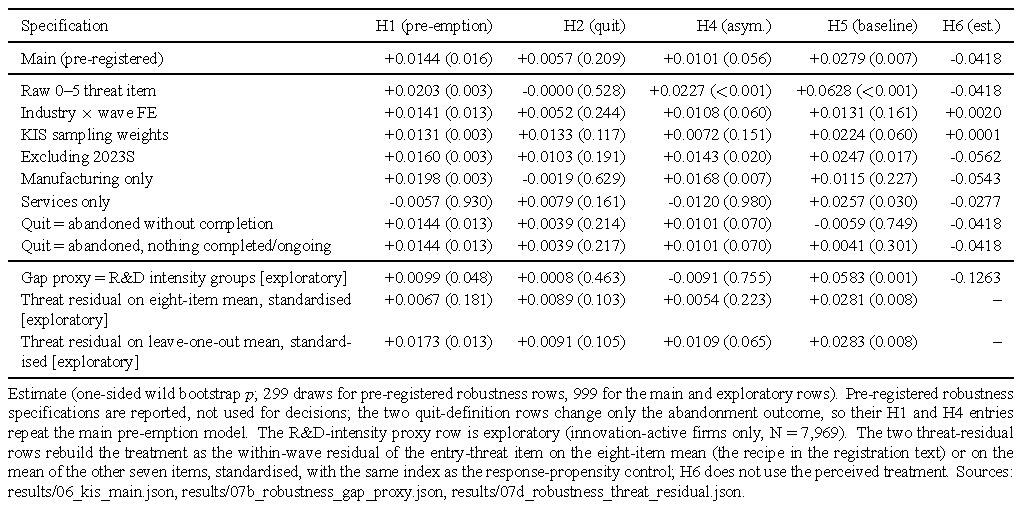
\includegraphics[max width=\textwidth]{tables_tex/T_robustness.pdf}
\end{table}

An exploratory row replaces the R\&D-staff proxy with R\&D expenditure over sales, grouped the same way and available only for the \AltN{} innovation-active firms; the two groupings agree on the diagonal for \AltDiagGZero, \AltDiagGOne{} and \AltDiagGTwo{} firms. There the escape slope is \AltHOneEst{} ($p$ = \AltHOneP) with the expenditure proxy and \AltHOnePreregSameSubEst{} ($p$ = \AltHOnePreregSameSubP) with the registered proxy, the baseline difference \AltHFiveEst{} ($p$ = \AltHFiveP), the exit-margin tests null (\AltHTwoEst, \AltHThreeEst, \AltHFourEst) and the H6 slope \AltHSixEst, as with the registered proxy. The last two rows rebuild the treatment. Residualised on the eight-item mean and standardised, the registration text's recipe, the frontier slope falls to \ResidMeanEightHOnePp{} percentage points ($p$ = \ResidMeanEightHOneP; interval \ResidMeanEightHOneLoPp{} to \ResidMeanEightHOneHiPp), because the index contains the treatment item; with the leave-one-out mean of the other seven items it is \ResidMeanSevenHOnePp{} ($p$ = \ResidMeanSevenHOneP; interval \ResidMeanSevenHOneLoPp{} to \ResidMeanSevenHOneHiPp), and the two residuals correlate \ThreatResidCorrMeanEight{} and \ThreatResidCorrMeanSeven{} with the registered one. The exit-margin slopes stay small under both (\ResidMeanEightHTwoPp{} and \ResidMeanSevenHTwoPp{} percentage points) and the baseline difference at \ResidMeanEightHFivePp{} and \ResidMeanSevenHFivePp. The escape association depends on the propensity index not containing the item it adjusts, which the registered construction satisfies; the attenuated figure is reported because a reader of the registration text would expect it.

\subsection{Placebo items and exploratory tests}

The two placebo items, residualised within wave on the eight-item mean and standardised as the registration text specifies (Section~\ref{sec:data}), are reported in Table~\ref{tab:placebo} with two-sided $p$-values. Demand unpredictability interacted with the laggard indicator gives \PlaceboDemandQuitEst{} on abandonment ($p$ = \PlaceboDemandQuitP) and, interacted with the frontier indicator, \PlaceboDemandPreEst{} on pre-emption ($p$ = \PlaceboDemandPreP); price sensitivity gives \PlaceboPriceQuitEst{} ($p$ = \PlaceboPriceQuitP) and \PlaceboPricePreEst{} ($p$ = \PlaceboPricePreP). The demand item's negative association with frontier pre-emption is the closest any placebo comes to significance, and its sign is opposite to the treatment's; a general tendency to rate the environment as uncertain would have produced a positive slope on both items.

\begin{table}[htbp]
\centering
\caption{Pre-registered placebo items and exploratory tests, same specification as the main models; two-sided wild bootstrap $p$-values. Sources: results/06\_kis\_main.json (placebo), results/07\_kis\_exploratory.json, generated by code/make\_tables.py.}
\label{tab:placebo}
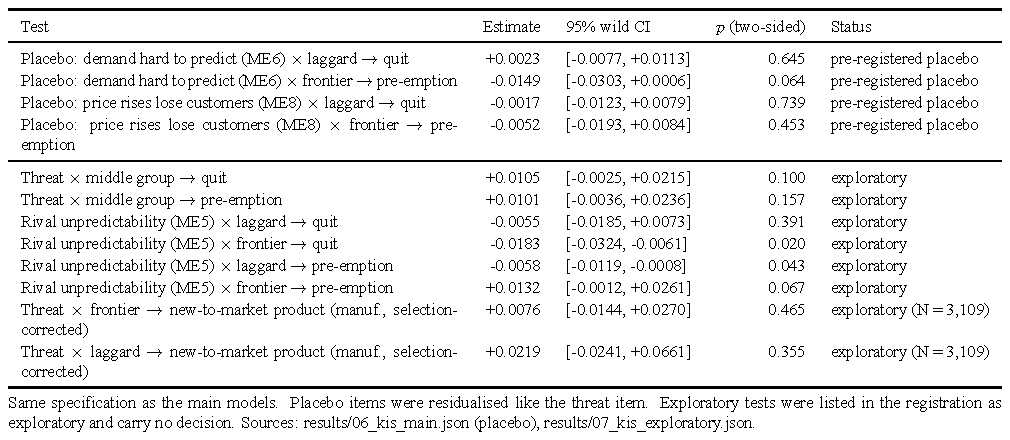
\includegraphics[max width=\textwidth]{tables_tex/T_placebo_exploratory.pdf}
\end{table}

The exploratory tests, listed as such in the registration, carry no decision. The middle group's slopes are \ExplGapOneQuitEst{} on abandonment ($p$ = \ExplGapOneQuitP) and \ExplGapOnePreEst{} on pre-emption ($p$ = \ExplGapOnePreP), close to the frontier group's on both margins. The rival-unpredictability item, for which the model gave no direction, is associated with less abandonment among frontier firms (\SigmaQuitGTwoEst, $p$ = \SigmaQuitGTwoP) and less pre-emption among laggards (\SigmaPreGZeroEst, $p$ = \SigmaPreGZeroP), with \SigmaQuitGZeroEst{} and \SigmaPreGTwoEst{} for the other two cells; these are two of four cells at conventional significance in an unregistered test and I draw nothing from them beyond their usefulness for a future registration. The selection-corrected test \citep{heckman1979sample} of new-to-market product innovation on the manufacturing product innovators (\MarketFirstN{} firms, selection equation on \MarketFirstNSel) gives a frontier slope of \MarketFirstGTwoEst{} ($p$ = \MarketFirstGTwoP); the model's `finishing first' is not visibly moved by perceived threat in these data.

\subsection{Theory, agents and firms side by side}

Set side by side (Table~\ref{tab:threeway}), the three columns agree in sign on the escape margin, with the firms' response far smaller than the agents' and in the same direction as the model's, and they agree on the baseline. On the exit margin the theory and all four agent arms, in both stages, predicted a positive laggard response and a positive asymmetry, and the firms show neither. On realised entry, theory and agents predicted no rise in pre-emption and the firms' estimate is negative but imprecise. The two contrasts on which the three columns disagree, H2 and H3, are the two in which the model's mechanism is a decision to stop before the entrant has arrived.

\begin{table}[htbp]
\centering
\caption{Three-way comparison of signs: theory, frozen agent consensus (Stage A and Stage B) and the pre-registered survey estimates. Source: results/06\_threeway\_table.json, generated by code/make\_tables.py.}
\label{tab:threeway}
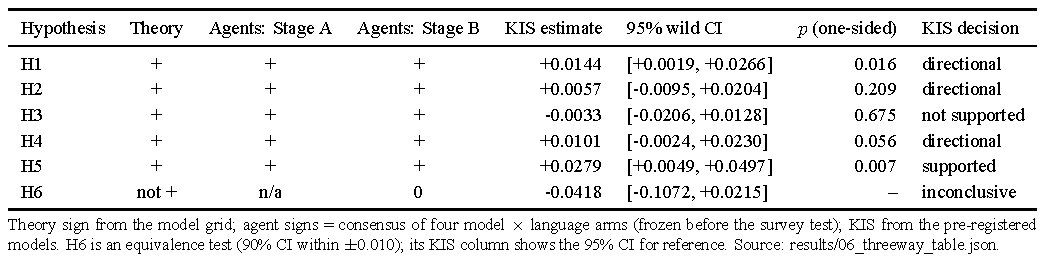
\includegraphics[max width=\textwidth]{tables_tex/T_threeway.pdf}
\end{table}

\section{Mechanisms: what the agents said}
\label{sec:mech}

Every agent decision came with a reason of at most two sentences: \CodesNReasons{} in all, \StageAReasonsAll{} from Stage A decisions and \StageBReasonsAll{} from Stage B periods. Two judge models coded each reason against a ten-category rubric derived from the model (\ref{app:rubric}; the categories head the columns of Table~\ref{tab:mech}). The judges are the same two models that wrote the reasons, each coding both models' output in batches of twenty-five, so their agreement is evidence about the legibility of the reasons and not an independent human reading; a fixed sample of fifty reasons is set aside in the public package for independent human validation. Both judges returned codes for \CodesN{} reasons (\CodesNotBothJudged{} were lost to a partial parse; \StageAReasons{} from Stage A, \StageBReasons{} from Stage B). Cohen's $\kappa$ ranges from \CodesKappaMin{} to \CodesKappaMax{} across categories (median \CodesKappaMedian; \KappaMTwo{} for threat-as-reason-to-hurry, \KappaMThree{} for threat-as-reason-to-stop, \KappaMSix{} for sunk cost or redirection), and the judges agree on the single primary label for \CodesPrimaryAgreePct\% of reasons; Table~\ref{tab:mech} reports, by stage and decision, the share of reasons both judges coded into each category, and \ref{app:judgeshares} gives the threat-cell shares by judge.

\begin{table}[htbp]
\centering
\caption{Stated reasons of the agents coded by two judge models, by stage and decision: share of reasons coded into each category by both judges, and inter-judge $\kappa$. Source: results/08\_transcript\_codes.json, generated by code/make\_tables.py.}
\label{tab:mech}
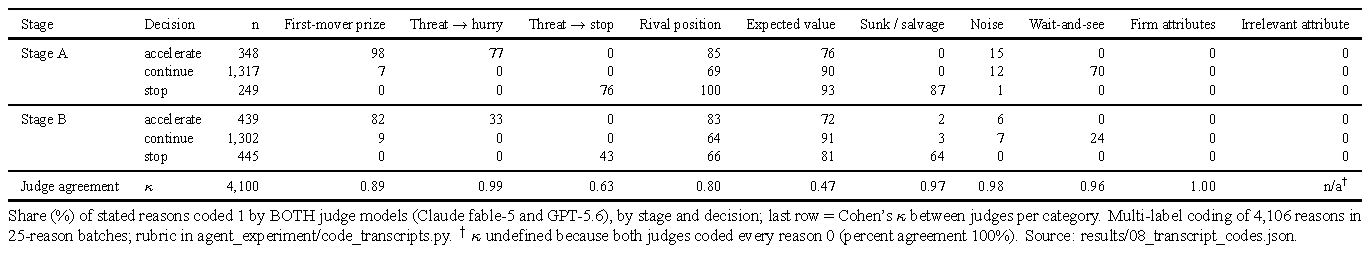
\includegraphics[max width=\textwidth]{tables_tex/T_mechanisms.pdf}
\end{table}

The reasons read as the model's backward induction in business language. A frontier persona in the threat cell that chose to accelerate wrote (\ExReasonAccelArm, design \ExReasonAccelId): `\ExReasonAccel' A laggard persona in the threat cell that chose to stop wrote (\ExReasonStopArm, design \ExReasonStopId): `\ExReasonStop' And a level persona without a threat that chose to continue wrote (\ExReasonContArm, design \ExReasonContId): `\ExReasonCont' The three are the first English Stage A reasons in design order with the stated decision, cell and code, quoted from the public logs. The shares bear the examples out: within the threat cells, \ShareAAccelThreatHurryPct\% of Stage A acceleration decisions name the entrant as the reason to hurry and \ShareAQuitThreatQuitPct\% of stop decisions as the reason to stop, and in cells without a threat both shares are zero; in Stage B the two shares are \ShareBAccelThreatHurryPct\% and \ShareBQuitThreatQuitPct\%, lower because the dynamic race also gives the agent the rival's observed position and money already spent to argue from. The firm attributes appear in \FirmAttrCount{} reason out of \CodesN{} and the placebo attribute in none, so neither the persona nor the irrelevant detail drove the choices, as the within-cell placebo tests had shown in behaviour.

The model's exit mechanism is a comparison between the continuation value of a project that will finish after the entrant and the value of redeploying its budget now; the agents performed that comparison, named both sides and stopped. The survey firms with no dedicated R\&D staff who rate the threat high did not report more abandoned or suspended activities than those who rate it low (\KISHTwoPp{} percentage points per standard deviation); what they report slightly more of is lead-time protection (\CoefPreXGZero{} in probability units, Table~\ref{tab:coef}). The agents' agreement with the model is therefore evidence about the model's logic, not about firms.

\section{Discussion}
\label{sec:discussion}

\subsection{What the three columns agree and disagree on}

The step-by-step literature has treated the escape response of near-frontier firms and the discouragement of laggards as two sides of one mechanism and tested them on patents and productivity \citep{aghion2005competition,aghion2009entry}. Carrying the mechanism into a finite race, giving the entrant a concrete effect (a cut in unfinished prizes) and observing abandonment directly, I find the first side and not the second. Frontier firms by the R\&D-staff proxy that perceive entry threat use lead-time protection more often, by about \KISHOneRelMeanPct\% of the sample rate and \KISHOneRelFrontierPct\% of their own; firms with no dedicated R\&D staff abandon more at any level of threat but no more when they perceive it as higher.

The exit-margin null admits three readings. The first is measurement: the abandonment item is answered only by innovation-active firms, so a laggard that responds to entry threat by not starting a project leaves no trace in it; the sample restriction, inherited from the CIS literature \citep{garciavega2010determinants,klingebiel2021optionality}, conditions on having been in the race, and no CIS-type survey records the project pipeline a deterrence test would need. The second is the proxy: firms without dedicated R\&D staff may be laggards in the model's sense or may simply innovate without R\&D staff, and the gap groups are far thinner in services (\SecGapNServTwo{} frontier firms) than in manufacturing (\SecGapNManuTwo); the exploratory expenditure proxy gives the same pattern, which weakens this reading without removing it. The third is behavioural: anticipatory stopping requires a firm to compute the continuation value of a project under a hypothetical entrant and act on it before the entrant arrives, as the agents' reasons in Section~\ref{sec:mech} do; firms may instead treat entry threat as background pressure that raises the value of protecting what they have (the escape response they do show) and abandon projects for the reasons the hampering-factor literature names, cost, knowledge and partnership difficulties \citep{garciavega2010determinants,lhuillery2009rd,deste2012what}, as laboratory followers close behind kept investing against the theory's advice \citep{zizzo2002racing,breitmoser2010understanding}. The design cannot separate the second and third readings, but it fixes the size of the response they would have to explain, a laggard abandonment slope below \MDEQuitPp{} percentage points per standard deviation against an escape slope of \RobManuHOnePp{} in manufacturing; a panel of the same firms or an item on projects not started because of expected entry would separate them.

The agent arm adds a measurement of the model's logic that is independent of the theorist in derivation, though not in setting: two frontier models, in two languages and two settings, with the theory's vocabulary removed from the prompt, reproduced the comparative statics of the race and explained them in its own terms, siding with the firms where they agree with the model and with the model where they do not. Given a fully described environment these models compute the backward-induction answer, which supports the use \citet{horton2023large} proposed and this study made, piloting predictions before registration, and tells against reading an agent experiment as evidence about firms; \citet{manning2024automated} observed that language models predict the signs of effects well and their magnitudes poorly, and the agents' Stage A responses were several times the model's and an order of magnitude above the firms'.

\subsection{Implications for management}

For a firm with a project near completion that sees entry coming, the escape response is the one associated with its position in Korean manufacturing, where the frontier slope is \RobManuHOnePp{} percentage points per standard deviation of perceived threat on a base rate of \PreemptRateTwoZeroTwoTwoMPct\% to \PreemptRateTwoZeroTwoFourMPct\%, and the model says why: a product launched before the entrant keeps its full margin while everything launched afterwards loses part of it, so the value of a month saved rises with the probability of entry. The finding suggests that budgeting for acceleration options (second shifts, parallel testing, pre-booked certification) is a reasonable response to a rise in perceived entry threat for projects in their last stage, and that the case for the same spending is weaker for projects far from completion, where the model predicts a smaller response and the survey slopes are smaller. For project portfolio managers the exit-margin result is a caution in the opposite direction. The race logic recommends stopping distant projects when entry looms, and the organisational literature on selective firms \citep{klingebiel2021optionality} shows that the capacity to stop is a capability; Korean firms do not appear to stop in anticipation: the laggard abandonment slope is \KISHTwoPp{} percentage points per standard deviation of perceived threat, so a manager who imports the race logic would abandon more readily than the firms in these data do, and the data record the abandonment but not its payoff.

\subsection{Implications for policy}

The policy implications carry the grade of a cross-sectional association, and I state them at that grade. Korean entry policy has a statutory home. The Support for Small and Medium Enterprise Establishment Act (Act No.~\LawSMESAActNo, in force \LawSMESAEffective) states as its purpose a start-up ecosystem in which anyone can start a firm on a creative idea or an innovative technology and grow it into a globally leading company, defines a start-up firm as an SME within seven years of commencing business, and in Article~\LawSMESARegArticle{} directs the Government to identify and relax or remove regulations that hinder start-ups or block their growth; the duty is one to endeavour, and the Act names no target entry rate. Where it raises the prospect of entry, these data associate perceived threat with more pre-emption among manufacturing frontier firms and no detectable change in abandonment among laggards. The range of realised entry across the industries in the sample is wide, from \EntryMinIndTwoZeroTwoFourMPct\% of active enterprises a year in \EntryMinIndTwoZeroTwoFourMLabel{} to \EntryMaxIndTwoZeroTwoFourMPct\% in \EntryMaxIndTwoZeroTwoFourMLabel{} in the 2024 reference period, and across that range the industry entry rate is not associated with more pre-emption and is associated with more abandonment in every gap group alike. The worry that competition policy discourages laggard incumbents does not take the form of abandoned projects here, within the design's power to detect a laggard slope of \MDEQuitPp{} percentage points per standard deviation; the laggards' higher abandonment is a level difference tied to the absence of dedicated R\&D staff, which points policy at R\&D capacity, not entry conditions. The instrument that already works on that margin is the credit for research and human-resource development expenses under Article~\LawRSTAArticle{} of the Restriction of Special Taxation Act (Act No.~\LawRSTAActNo): for an SME's general research and human-resource development expenses it returns, at the taxpayer's choice, \LawRSTASMECurrentPct\% of the year's expenses or \LawRSTASMEIncrementPct\% of their increase over the previous year (\LawRSTAMidCurrentPct\% and \LawRSTAMidIncrementPct\% for middle-standing enterprises, and for other firms a revenue-ratio formula capped at \LawRSTALargeCapPct\%), with eligible expenses defined by Presidential Decree. The data identify the group that abandons more, the \GapZeroN{} firms with no dedicated R\&D staff, and not the effect of the credit on it; whether the credit reaches firms that have no R\&D staff to begin with is the question a programme evaluation would have to ask. The escape association is absent in services, where \PreemptRateTwoZeroTwoFiveSPct\% to \PreemptRateTwoZeroTwoThreeSPct\% of firms report lead-time protection and \ShareZeroRDServMinPct--\ShareZeroRDServMaxPct\% have no dedicated R\&D staff, so a policy expecting service incumbents to answer entry with faster innovation has no support here, and a protection-method item written for product innovation may be the wrong instrument there. For the survey agencies the suggestion is narrower: the market-environment block shared with the European CIS 2020 questionnaire is informative once response propensity is removed, and an item on projects not started because of expected entry would make the deterrence margin observable, where the present item sees only the \NQuitSample{} firms already racing.

\subsection{Limitations}

The data are repeated cross-sections, so every estimate is an association between a perception at the time of the survey and a behaviour reported over the same three-year window; perceptions may follow behaviour (a firm that has just abandoned a project may rate the threat higher), and no instrument for perceived threat is available in these files. The response-propensity adjustment and the placebo items do not exclude a firm-specific shock that raises both perceived threat and lead-time protection; the stability of the escape coefficient across the registered control sets could be turned into a formal bound on selection on unobservables \citep{oster2019unobservable}, which I have not done. The gap proxy is the share of dedicated R\&D staff, not distance to completion; it separates firms with and without formal R\&D well, the two upper groups less well, and degenerates in services. The outcomes are survey items: `abandoned or suspended' pools permanent stops with pauses, and `entering the market ahead of competitors' is a protection method the firm reports using, not an observed acceleration. The agents are two models at one point in time, called at default sampling (no temperature or top-p was set; the defaults are not in the API documentation consulted) and given a fully specified environment that real managers never have; their agreement with the theory shows what the models compute, not what firms do, and the Stage B placebo check lost independence across models through the shared episode seed. The industry entry rate is a national two-digit birth rate, closer to turbulence than to the technologically advanced entry of the model and of \citet{aghion2009entry}. The power analysis fixes what the nulls mean: the design detects laggard abandonment slopes of about \MDEQuitPp{} percentage points per standard deviation, so smaller responses are not excluded, and the H6 interval is too wide for the registered equivalence band; `directional' for H1 reflects a Holm adjustment across five tests, not an estimate near zero.

A panel with firm identifiers across KIS or CIS waves would observe the same firm's threat perception and abandonment in sequence and separate deterrence from abandonment; the European CIS 2020 microdata carry the identical market-environment block and abandonment item, so the two-margin test can be repeated across entry regimes; and the agent protocol can be inverted, asking what must be removed from the environment description (the entry probability, the prize halving, the rival's position) before the agents stop computing the race and behave like the survey firms, which would locate the behavioural gap in the information managers have.

\section{Conclusions}

A finite-horizon innovation race with an entrant that taxes unfinished prizes predicts two responses to the threat of entry, pre-emption by firms close to completion and abandonment by firms far from it, from one mechanism and without different preferences for the two types of firm. The hypotheses were registered before the survey test together with the frozen predictions of two LLM agents and taken to four waves of the Korean Innovation Survey with the CIS entry-threat item, the abandonment item and the lead-time protection item. Perceived entry threat is associated with more lead-time protection among frontier firms in manufacturing, by about \KISHOneRelMeanPct\% of the sample rate; it is not detectably associated with more abandonment among laggards, and the asymmetry in abandonment that theory and agents predicted is absent; laggards abandon more at every threat level; and realised entry is not associated with more pre-emption, although the equivalence test is inconclusive. The disagreement between the firms on one side and the model and the agents on the other is confined to the stop decided in anticipation of entry. Whether Korean laggards do not make that decision, or make it before a project is started and so outside the survey's view, cannot be told from repeated cross-sections; the design that could tell is a panel of the same firms, or an item on projects not started, and the effect it would have to find is smaller than \MDEQuitPp{} percentage points per standard deviation.

\appendix

\section{The race model: specification, two-period derivation and numerical check}
\label{app:model}
\setcounter{equation}{0}
\renewcommand{\theequation}{A.\arabic{equation}}

\paragraph{State and timing} The state is $(t, x_L, s_L, x_F, s_F, e)$ with $t \in \{1, \ldots, T\}$, positions $x_i \in \{0, \ldots, K\}$, status $s_i \in \{\text{active}, \text{stopped}, \text{finished}\}$ and entry indicator $e \in \{0, 1\}$. Each period: (i) if $e = 0$, entry occurs with probability $\theta$ and sets $e = 1$; (ii) active firms choose intended actions simultaneously from $\{Q, C, A\}$; with the rival-unpredictability parameter $\sigma > 0$ an intended $C$ or $A$ is re-drawn uniformly from $\{C, A\}$ with probability $\sigma$ (implementation tremble), $Q$ is never disturbed; (iii) costs are paid and progress realised, a firm reaching $x_i = K$ receives its prize ($V$ if the rival has not finished, $W$ if it has, $(V+W)/2$ if both finish in the same period, each multiplied by $\lambda^{e}$) and becomes finished, a firm realising $Q$ becomes stopped; (iv) $t$ advances, and all values are zero at $T + 1$. Convexity requires $c_A / c_C > p_A / p_C$ with $p_A > p_C$ and $c_A > c_C$. The discount factor is one.

\paragraph{Equilibrium and selection} With one active firm the problem is a single-agent maximisation, ties broken towards the lower effort. With two, the stage game is the three-by-three bimatrix game with payoffs equal to minus the cost plus the expected prize and continuation value; all pure Nash equilibria are enumerated and, if none exists, mixed equilibria are found by support enumeration. Multiple equilibria (\ModelMultiShare\% of solver runs, \ModelMixedShare\% mixed) are resolved by the main rule, which prefers the equilibrium with the largest joint payoff, then the one with fewer expected accelerations, then the one in which the firm farther from completion (the follower if equal) takes the lower effort; in symmetric states a symmetric equilibrium is preferred and mirror pairs are resolved by a fair coin. The leader-preferred and follower-preferred rules are reported as alternatives, and no registered sign depends on the rule.

\paragraph{Outcomes} Outcome probabilities are computed by exact propagation of the state distribution, not by simulation; the distribution is augmented with indicators for having intended $A$ at least once. The threat-conditional version propagates only the branch without entry within the horizon and renormalises by $(1-\theta)^{T}$; a Monte Carlo replication with \MCPaths{} paths agreed with the exact propagation within \MCMaxDiff{} on every outcome probability, and the \ModelControlsCount{} controls run before the grid (two-route agreement with the closed form, $\lambda = 1$ and $\theta = 0$ invariances, the deterministic $\varepsilon$-preemption limit, label symmetry at zero gap, mass conservation, probability identities, agreement of the two $\sigma$ definitions at $\sigma = 0$, and the conditional-outcome identity) all pass.

\paragraph{Two-period case} Let $T = 2$, $K = 2$, $x_{L0} = 1$, $x_{F0} = 0$, $\sigma = 0$, $s(e) = \lambda^{e}$, $M = (V+W)/2$, and for a firm alone with one stage left and prize $R$ let $g(R) = \max\{0,\, -c_C + p_C R,\, -c_A + p_A R\}$. Period 2, given the entry status $e_2$ and $s = s(e_2)$: if the leader has finished and the follower is at 1, the follower is alone with the second prize, $v_F^{2a}(s) = g(Ws)$; if the leader has finished and the follower is at 0, the follower cannot finish and earns nothing; if neither has finished and both are at 1, the last-period duel has payoffs
\begin{equation}
u_i(a_i, a_j) = -c(a_i) + p(a_i)\, s\,\bigl[V - p(a_j)(V - M)\bigr],
\end{equation}
so each firm's best response is a threshold rule in the rival's effort, and the Nash equilibrium is selected as above; if the leader is at 1 and the follower at 0, the follower stops and the leader is alone, $v_L^{2d}(s) = g(Vs)$; if the leader stopped in period 1 and the follower is at 1, the follower is alone with the first prize, $g(Vs)$. Period 1, with $s_1 = s(e_1)$ and $E_2$ the expectation over $e_2$ ($e_2 = 1$ with probability $\theta$ if $e_1 = 0$, with certainty otherwise):
\begin{align}
u_L(a_L, a_F) &= -c(a_L) + p_L V s_1 + (1 - p_L)\bigl[p_F\, E_2 u_L^{2c} + (1 - p_F)\, E_2 v_L^{2d}\bigr], \\
u_F(a_L, a_F) &= -c(a_F) + p_F\bigl[p_L\, E_2 v_F^{2a} + (1 - p_L)\, E_2 u_F^{2c}\bigr] \quad (a_L \neq Q),
\end{align}
with $p_F = 0$ if $a_F = Q$ and $u_F = -c(a_F) + p_F\, E_2\, g(Vs_2)$ if $a_L = Q$. The period-1 equilibrium is the Nash equilibrium of this game.

\paragraph{Proposition 1 (exit)} The follower's value from $C$ is $-c_C + p_C \Phi_F(\theta)$ with $\Phi_F$ as in Eq.~(\ref{eq:phi}). $v_F^{2a}$ and $u_F^{2c}$ are non-decreasing in $s$, and $s(1) = \lambda < 1 = s(0)$, so if the leader's period-2 action does not depend on $e_2$, $\Phi_F$ is non-increasing in $\theta$ and there is a threshold $\theta^{*}$ with the follower stopping if and only if $\theta \ge \theta^{*}$.

\paragraph{Proposition 2 (escape)} The leader prefers $A$ to $C$ in period 1 if and only if condition (\ref{eq:accel}) holds, $(p_A - p_C)[V s_1 - \Psi_L(\theta)] > c_A - c_C$, with $\Psi_L$ as in Eq.~(\ref{eq:psi}). Under the same condition $\Psi_L$ is non-increasing in $\theta$, so the gain from finishing now rather than later is non-decreasing in $\theta$ and a threshold $\theta^{**}$ exists above which the leader accelerates.

\paragraph{Where monotonicity fails} Both propositions hold under the condition that the rival's period-2 action is insensitive to the entry draw. When it is not, for instance when a leader that would accelerate in a last-period duel without entry prefers $C$ once the prize is cut, $\Phi_F$ can rise with $\theta$ over an interval; and a small $\theta$ can make the follower stop, which lowers the leader's need to accelerate before the leader's own threshold is reached, so the leader's acceleration probability need not be monotone even where its end-point sign is right. The grid in Section~\ref{sec:theory} measures how often each failure occurs.

\paragraph{Numerical check} A check script (code/model\_check.py, results/model\_check.json) re-derives the statements above from the solver. In the two-period case at a representative parameter point (the calibrated environment's prizes, costs and $\lambda$), the closed-form and the general solver agree on values and outcome probabilities to \ModelCheckTwoRouteGap{} at every point of a $\theta$ grid from zero to \ModelCheckThetaGridMax; the period-1 game is a mixed war of attrition at $\theta = 0$ (follower stops with probability \ModelCheckTwoPeriodQuitAtZero, leader accelerates with probability \ModelCheckTwoPeriodAccelAtZero), the follower's stopping probability is weakly increasing in $\theta$ and reaches one from $\theta$ = \ModelCheckThetaStar{} onwards, and the leader accelerates with certainty from $\theta$ = \ModelCheckThetaTwoStar{} onwards after the non-monotone stretch described above. In the calibrated three-period environment, with central differences on a fine $\theta$ grid, the frontier leader's threat-conditional acceleration rises from \ModelCheckLeaderAccelCondZero{} to \ModelCheckLeaderAccelCondSeven{} while its unconditional acceleration falls from \ModelCheckLeaderAccelUncondZero{} to \ModelCheckLeaderAccelUncondSeven; the laggard's abandonment rises from \ModelCheckLaggardQuitUncondZero{} to \ModelCheckLaggardQuitUncondSeven{} and exceeds the leader's (\ModelCheckLeaderQuitUncondZero) at $\theta = 0$; the choice set contains the option to wait (continue); and the $\lambda = 1$ and $\theta = 0$ invariances hold. All checks \ModelCheckAllPass.

\section{Survey items and coding notes}
\label{app:items}
\setcounter{table}{0}
\renewcommand{\thetable}{B.\arabic{table}}

Table~\ref{tab:variables} in the main text lists every item with its verbatim questionnaire wording, the variable names in the four provision files, the English label used in this paper and its role. Four coding notes complete it. First, the four questionnaires print the market-environment block, the protection-method block, the innovation-activity block and the workforce block with identical wording apart from the reference years, and this was verified item by item against the text extracted from each questionnaire; the response scale of the market-environment block is 0 `not applicable', 1 `very low', 2 `low', 3 `moderate', 4 `high', 5 `very high'. Second, the 2023 services file departs from the printed codes: the 0--5 scales are stored as 1--6, yes/no items as 1/2 rather than 1/0, the funding-source scale 0--3 as 1--4, and `not applicable' as a four-digit code; each recode was derived by comparing observed value frequencies with the printed codes and is recorded in the item map, and a test reproduces every observed frequency from the recoded data. Third, two codebook descriptions in the 2024 and 2025 files repeat text from another question for the first market-environment item; the questionnaire wording was taken as authoritative and the discrepancy is documented in the maps. Fourth, two undocumented values are treated as missing rather than read as data: a sentinel (\SentinelValueRDExp) in the R\&D-expenditure fields of the 2024 file and one founding year of 30 in the 2025 file. The register fields used are the two-digit industry code, the employee-size band, the founding year and the sampling weight; the industry division is mapped to its KSIC section letter and cross-checked against the register's own section variable where one exists, with no disagreements.

\section{The agent experiments: protocol, calibration, design history, prompts and coding rubric}
\label{app:prompts}

\subsection{Call protocol and controls}
\label{app:protocol}

Both models were called through Amazon Bedrock without a system prompt and at the providers' default sampling (no temperature or top-p was set). The Stage A calls were made on \StageACallsDate{} between \StageACallsFirstKST{} and \StageACallsLastKST{} KST and the Stage B calls on \StageBCallsDate{} between \StageBCallsFirstKST{} and \StageBCallsLastKST{} KST; every call is logged with its prompt hash, prompt, raw response, parsed decision and option order, and every episode with every environment draw. Each firm profile (persona) was drawn from a KIS record using four treatment-free register attributes: the two-digit industry, whose codebook title the prompt shows and which fixes the sector, the employee-size band, firm age and group affiliation. The three options were shown in a random order that was logged, because a content-free probe (three lettered options and no reason to prefer any) had returned the first option in \ProbeFableFirstOption{} of \ProbeFableCalls{} calls from Claude and \ProbeGptFirstOption{} of \ProbeGptCalls{} from GPT-5.6, with `the first option' given as the reason. A frontier model will recognise a race from a payoff table whatever the race is called, so the forbidden-vocabulary check (\ref{app:vocabulary}) cannot hide the structure of the problem; what it does is keep the theory, the predicted direction and the literature out of the prompt.

Before any choice is read, the design is checked against its own nulls. The placebo attribute (the month of the firm's founding anniversary) and the option-position effect form one null family per stage, tested within cells by re-randomisation (placebo labels permuted within cell, two thousand draws) with Holm adjustment across the arms; the smallest adjusted $p$-value is \StageAPlaceboMinHolm{} in Stage A and \StageBPlaceboMinHolm{} in Stage B. The Stage B check carries a caveat that is a design lesson: environment draws are seeded by episode index, which the two models share within a language, so when the Claude--Korean placebo contrast came out at \StageBPlaceboMinRaw{} before adjustment it was because the placebo-one episodes in that language happened to receive luckier rival draws, for both models alike; the two arms of a language are therefore not independent replications of the placebo check. Finally, a scripted agent playing the equilibrium policy was passed through the full prompt-and-parse pipeline and reproduced the model's cell outcomes, so the runner itself does not distort behaviour.

\subsection{Calibrating the environment before any call}
\label{app:calibration}

The Stage B environment is the three-period race of Section~\ref{sec:theory} in money units, so that the agents play the model itself rather than a story about it: \EnvStages{} development stages and \EnvPeriods{} periods; continuing costs \EnvContinueCostBn{} billion won (\EnvContinueCost{} in the Korean unit of a hundred million won, which the Korean prompts use) with a \EnvContinueSucc\% chance of completing a stage, accelerating \EnvAccelCostBn{} billion won with \EnvAccelSucc\%, stopping nothing; profit of about \EnvPrizeFirstBn{} billion won if the firm launches before the rival, \EnvPrizeSecondBn{} billion if after, \EnvPrizeTieBn{} billion each if in the same period, nothing if unfinished; in threat games a new competitor enters with probability \EnvTheta\% at the start of each period and halves the profit of every product not yet launched ($\lambda$ = \EnvLambda); in noise games the rival's stage is reported with a one-stage error \EnvNoise\% of the time. The rival follows the equilibrium policy of the solved model at the true state, so the agent faces the opponent the theory assumes, and the coordination failures that \citet{akata2025playing} document in the Battle of the Sexes, where two models have to settle on one of two equilibria, cannot arise, because the rival's play is fixed. The twelve cells cross three positions (one stage behind, level, one stage ahead), the threat and the observation noise.

One parameter was calibrated, by a rule fixed before the scan was read. At the draft acceleration cost of \EnvDraftAccelCostBn{} billion won the model's own leader, one stage from completion, accelerated with probability \EnvDraftLeaderAccelNoThreat{} already without any threat: the environment sat on the model's ceiling for the escape comparative static, and an experiment there could not have shown the predicted effect even from agents that behaved like the model. Holding every other parameter fixed, I scanned the acceleration cost on a grid of 0.5 billion won and chose the smallest value at which, in the model, the frontier leader's threat-conditional acceleration probability without threat lay between 0.20 and 0.80 and rose by at least 0.05 with the threat, the laggard's abandonment probability met the same two conditions, the laggard abandoned more than the leader, and convexity held. The only value that passed was \EnvAccelCostBn{} billion won. The rule evaluated the leader on the threat-conditional outcome, which is the survey item's counterpart, and the laggard on the unconditional outcome, which the model predicts in both versions; at the chosen value the model gives, for the agent's seat, frontier acceleration of \EnvLeaderAccelNoThreat{} without threat and \EnvLeaderAccelThreat{} with it conditional on no entry, laggard abandonment of \EnvLaggardQuitNoThreat{} without threat and \EnvLaggardQuitThreat{} with it unconditionally, and leader abandonment of zero; Table~\ref{tab:env} gives both versions for every cell.

\subsection{Design history: two discarded vignettes}
\label{app:design}

The registered vignette is the third version, and the two earlier versions are documented with their logs because each produced a result clean enough to be suspected of being an artefact, and in each case it was one. The first version told the race qualitatively, with a large reward for launching first and no concrete costs, second prize or value of stopping; in a pilot of \VOnePilotCalls{} calls the two models chose acceleration in \VOneAccelMinPct--\VOneAccelMaxPct\% of cells, a ceiling that left nothing for the treatments to move. The second version added qualitative costs (`borrow about 40\% of the annual R\&D budget'), described the second prize as `barely covering the remaining development cost' and used a head-office move as the placebo attribute. In the full run of \VTwoCalls{} calls it produced a second ceiling, abandonment in \VTwoGapZeroQuitMin--\VTwoGapZeroQuitMax{} of the laggard cells, because the second-prize wording was my own approximation and not what the environment pays (\EnvPrizeSecondBn{} billion won against at most \EnvAccelCostBn{} billion of remaining continuation cost). It also produced a placebo effect, which was diagnosed before being believed. The first summary used a marginal contrast over all cells; the placebo had been randomised within persona and cell and its share happened to range from \VTwoPlaceboShareMin{} to \VTwoPlaceboShareMax{} across cells whose acceleration rates ranged from zero to one, so the marginal contrast (\VTwoFableEnMarginal{} in the Claude--English arm) inherited the imbalance. The within-cell contrast was \VTwoFableEnStratified{} in that arm ($p$ = \VTwoFableEnStratifiedP), concentrated in one cell, and the pooled within-cell contrast over the four arms had $p$ = \VTwoPooledAccelP. A head-office move is not decision-irrelevant on its face, since a firm that has just moved into a new building has shown that it can fund a large outlay, so the placebo was changed to the month of the founding anniversary, and the third version states the period-one decision of the calibrated environment in business language with the same numbers, so that nothing in the payoff description is approximated by hand. A control checks that every number in the templates equals the environment constant.

\subsection{Parse failures and the refusal diagnosis}
\label{app:refusal}

Of the \StageACalls{} Stage A calls, \StageAParseFail{} returned no parseable JSON and is kept as missing. Of the \StageBEpisodes{} Stage B episodes, \StageBComplete{} completed and \StageBParseFailed{} ended unparsed. The unparsed episodes were all in the Claude--Korean arm (\StageBFailedFaKo; GPT-5.6 had none) and were not a token problem: a direct probe showed the provider's `refusal' stop reason with zero output tokens, deterministic for the prompt text, so the affected prompts were replayed from the start and the residue is kept as missing rather than dropped.

\subsection{Agent shares not shown in the tables}
\label{app:agentshares}

In Stage A laggards stopped more than frontier firms by \SAHFiveMin{} to \SAHFiveMax{} across the four arms (the H5 contrast), and agents in level positions almost always continued. Across the whole of Stage A the two models differed in how readily they stopped, not in the direction of any contrast: Claude stopped in \SAOverallQuitFaEnPct\% (English) and \SAOverallQuitFaKoPct\% (Korean) of decisions, GPT-5.6 in \SAOverallQuitGpEnPct\% and \SAOverallQuitGpKoPct\%, with GPT-5.6 continuing in about four decisions out of five.


\subsection{Stage A vignette (version 3, English)}
\label{app:vignette}

The Korean primary template is identical in content and is published with the logs. Fields in braces are filled from the persona and the cell; bullets and line breaks of the template are removed here.

\begin{quote}\small
You are the executive responsible for new-product development decisions at a company in Korea. Read the situation below and make a decision.

[Company] Industry (Korean standard industrial classification title, as registered): \{industry\}. Size: \{size\}. Founded \{age\} years ago; \{group\}. The company's founding anniversary is in \{March / September\}.

[The project] Your company is developing a new product, and one rival is developing a comparable product. Development consists of 3 stages; once all 3 stages are completed the product is launched immediately. At most 3 development periods remain. In each period, each company chooses one of the following: Continue: cost 0.8 billion won, 50\% chance of completing one stage in that period. Accelerate: cost 2.5 billion won, 80\% chance of completing one stage in that period. Stop: cost 0, abandon the development for good and redirect the remaining budget and staff to the existing business. The cost is incurred in that period whether or not the stage is completed. The rival has the same options with the same costs and probabilities, and acts to maximise its own profit. Expected profit: about 10 billion won if you launch before the rival, about 3 billion won if you launch after the rival has launched, and 6.5 billion won each if both launch in the same period. If you do not complete within the 3 periods, there is no profit. (Profit figures are before development costs.)

[Current situation --- decision for the first period] \{gap: `Your company has completed 2 of the 3 stages; the rival is understood to have completed 1. You are one stage ahead.' / `Both your company and the rival are understood to have completed 1 of the 3 stages. The two companies are level.' / `Your company has completed 1 of the 3 stages; the rival is understood to have completed 2. You are one stage behind.'\} \{noise: `How many stages the rival has completed is known exactly from industry information. The rival also knows your progress exactly.' / `How many stages the rival has completed is an estimate from industry information; about 4 times in 10 it is off by one stage. The rival's picture of your progress is equally imprecise.'\} \{threat: `There is no possibility that a new competitor enters your market.' / `A new competitor with a comparable product may enter your market with a 35\% probability at the start of each period. It has not entered in this period. If entry happens, the expected profits of any product not yet launched at that time (10 / 3 / 6.5 billion won) are halved. Products already launched are not affected.'\}

[Decision] Choose one of the following for this period. In the next period you will decide again with new information. \{options in random order, lettered A, B, C\}

Answer only in this JSON format and write nothing else: \{``decision'': ``A'' or ``B'' or ``C'', ``reason'': ``at most two sentences''\}
\end{quote}

\subsection{Stage B templates (English)}

The rules block repeats the project description above with `There are 3 development periods in total', adds `You cannot see which option the rival chose, only its progress', and in threat games states that the entrant, once entered, stays. Each period the agent receives a history block (`Period \{t\}: you chose `\{act\}' and spent \{cost\} billion won; \{you completed a stage / you did not complete the stage\}. At the end of that period the rival \{is understood to have completed \{x\} of the 3 stages (estimate) / has abandoned its development for good / has already launched\}. New-competitor entry at the time of that decision: \{none / yes / not applicable\}.'), a state block (`Your company: \{x\} of 3 stages completed. Spent on development so far: \{spent\} billion won. Rival: \{status\}. New competitor: \{has not entered yet / has entered. Expected profits of products not yet launched are now halved (5 billion won if first, 1.5 billion won if after the rival, 3.25 billion won if simultaneous) / no possibility of entry\}. If you launched now, expected profit: \{amount\}.'), and the same decision block.

\subsection{Forbidden vocabulary}
\label{app:vocabulary}

Templates are checked against a list that includes `escape', `patent race', `race', `laggard', `leader', `Aghion', `game', `equilibrium', `Nash', `preempt', `Schumpeter', `incumbent', `deterrence' and their Korean equivalents.

\subsection{Coding rubric}
\label{app:rubric}

The judges received the scenario in two sentences and coded each reason on ten binary categories and one primary label: M1 first-mover prize (wants to launch before the rival or win the larger prize); M2 threat as a reason to hurry (the possible entrant and the profit halving given as a reason to speed up or finish sooner); M3 threat as a reason to stop (the possible or realised entrant given as a reason to stop or not invest further); M4 rival position (reasoning from the rival's stage, the chance of being overtaken or of catching up); M5 expected value (explicit cost--benefit or expected-value arithmetic); M6 sunk cost or salvage (money already spent, or redirecting budget and staff to the existing business); M7 noise (unreliability of the information about the rival's progress); M8 wait-and-see (keeping options open or deciding later as a reason to continue rather than accelerate); M9 firm attributes (industry, size, age or group affiliation); M10 irrelevant attribute (the founding-anniversary month or any other decision-irrelevant attribute). Reasons were coded in batches of twenty-five, in their original language, with the instruction to code what the text says and not what a rational agent should have said; known-answer texts were coded correctly by both judges before the run.

\subsection{Transcript shares within threat cells and by judge}
\label{app:judgeshares}

The shares below are over the \CodesN{} reasons coded by both judges. In Stage A, \ShareAAFirstMoverPrizePct\% of acceleration decisions name the first-mover prize and \ShareAAThreatHurryPct\% name the entrant as the reason to hurry; within the threat cells the latter share is \ShareAAccelThreatHurryPct\% (\JudgeAAccelThreatHurryFablePct\% by the Claude judge and \JudgeAAccelThreatHurryGptPct\% by the GPT-5.6 judge over \JudgeAAccelThreatHurryN{} decisions), and in cells without a threat it is zero. Stop decisions are the mirror image: \ShareAQThreatQuitPct\% cite the entrant as the reason to stop, \ShareAQuitThreatQuitPct\% within the threat cells, where the two judges coincide (\JudgeAStopThreatQuitFablePct\% and \JudgeAStopThreatQuitGptPct\% over \JudgeAStopThreatQuitN{} decisions) despite the category's $\kappa$ of \KappaMThree{} over all reasons; \ShareAQSunkOrSalvagePct\% cite redirecting the budget and staff to the existing business, and every one of them (\ShareAQRivalPositionPct\%) reasons from the rival's position. Continue decisions are the option to wait made explicit: \ShareACWaitAndSeePct\% give keeping the option open and deciding with new information as the reason, and \ShareACExpectedValuePct\% show expected-value arithmetic. In Stage B the shares are lower but ordered the same way: \ShareBAccelThreatHurryPct\% of threat-cell accelerations (\JudgeBAccelThreatHurryFablePct\% and \JudgeBAccelThreatHurryGptPct\% by judge) and \ShareBQuitThreatQuitPct\% of threat-cell stops (\JudgeBStopThreatQuitFablePct\% and \JudgeBStopThreatQuitGptPct\%) name the entrant; in the dynamic race the stop decisions are more often argued from the rival's observed position (\ShareBQRivalPositionPct\%), from expected-value arithmetic (\ShareBQExpectedValuePct\%) and from money already spent or redeployable (\ShareBQSunkOrSalvagePct\%), the three things the period prompts put in front of the agent.

\section{Deviations from the pre-registration and the embargo log}
\label{app:deviations}

\paragraph{Confirmatory analysis} None. The analysis script registered on \OSFRegisteredDate{} (SHA-256 recorded in the registration) was executed without modification on the real outcomes after the registration timestamp; the six decisions in Table~\ref{tab:main} are its output.

\paragraph{Description of the treatment in the registration text} The registration text (the `Transformations' entry of the registered document and the corresponding field of the OSF form) describes the perceived-threat treatment as the within-wave residual of the entry-threat item on the eight-item mean, standardised. The registered loader, whose output the registered analysis script consumes and whose code is part of the registered package, builds it as the within-wave residual of the item on the other seven items of the block, entered separately, without re-standardisation (pooled SD \ThreatResidSDPooled). The code is what ran and what the decisions in Table~\ref{tab:main} rest on; the text was written from the author's recollection of the design decision rather than generated from the code, and the mismatch was found while drafting this manuscript. It is reported here as a discrepancy between the registered text and the registered code, not as a change to the analysis, and both readings of the text's recipe are estimated as exploratory rows in Table~\ref{tab:robust}: residualising on the eight-item mean (which contains the item) gives a frontier slope of \ResidMeanEightHOnePp{} percentage points ($p$ = \ResidMeanEightHOneP), residualising on the mean of the other seven items gives \ResidMeanSevenHOnePp{} ($p$ = \ResidMeanSevenHOneP). The two placebo items were built by the registered script with the text's recipe (eight-item mean, standardised) and are reported as such.

\paragraph{Additions after registration} Two analyses were added and are labelled exploratory wherever they appear: the robustness row in Table~\ref{tab:robust} that replaces the R\&D-staff gap proxy with R\&D expenditure over sales, and the rubric coding of the agents' stated reasons in Section~\ref{sec:mech} (the registration listed the coding as an exploratory item without fixing the rubric). The numerical model check of \ref{app:model} was added for the manuscript and changes no registered quantity.

\paragraph{Embargo log} The registration uses the OSF Secondary Data Preregistration template. The registered package contains the loader with its refusal of outcome-by-treatment statistics (the loader keeps outcome and treatment columns in separate frames and refuses any cross-tabulation between them), the pre-registration marginals file with its embargo field, which records that no joint statistic was computed, the analysis script with its refusal to run on real outcomes unless a registration record with an OSF URL and timestamp exists, and the session log of the project. Statistics computed before registration, and disclosed in it, were outcome base rates by wave and size band, the distributions of the eight market-environment items and of the R\&D-staff share, correlations among explanatory items (including the \CorrThreatPlacebo{} correlation between the entry-threat and demand-unpredictability items that motivated the response-propensity adjustment), cluster and event counts, and the synthetic-outcome power analysis, which gave minimum detectable interaction slopes at 80\% power of \MDEQuitPp{} percentage points for abandonment and \MDEPreemptPp{} for pre-emption; none combines an outcome with a treatment. The registration is embargoed until \OSFEmbargoEnd{}; \ifanon its time-stamped record is available to the editor through the title page, and referees have the anonymised copy at \url{\OSFReviewCopyURL}\else a view-only link is provided to the editor and referees\fi.

\paragraph{Controls run before registration} The ordering of the two inference procedures was decided by a permutation control: with real outcomes permuted within wave and sector (\PermDraws{} draws) the two-sided cluster-robust $t$ rejected at nominal 5\% in \PermHSixClusterT{} of draws for the entry-rate slope of H6 and \PermHTwoObjClusterT{} for the objective H2 slope, against \PermHSixWild{} and \PermHTwoObjWild{} for the wild cluster bootstrap-$t$, the familiar over-rejection for a regressor that varies only at the cluster level \citep{cameron2008bootstrap}. A known-answer run on synthetic outcomes with planted slopes of \SimTrueHOne{} (pre-emption, frontier) and \SimTrueHTwo{} (abandonment, laggard) returned \SimHOneEst{} and \SimHTwoEst, and the planted placebos returned zero.

\section{Disclosure control for the public agent logs}
\label{app:disclosure}

The personas were drawn from individual KIS records using four register attributes (two-digit industry, employee-size band, exact firm age and group affiliation). Within the KIS sample, \PersonasUniqueInKIS{} of the \StageAPersonas{} personas match exactly one respondent on those attributes and \PersonasKLeThree{} match three or fewer, so publishing the prompts verbatim would publish individual-level records covered by the research-use licence. The public logs therefore replace the four company lines of every prompt (\RedactedPrompts{} prompts across the Stage A and Stage B files, including the discarded template versions) with a persona identifier, and \RedactedResponses{} agent responses that echoed an industry name or an exact age were redacted at the same positions; a scan confirms that no attribute string survives in the public files. The public persona table coarsens the attributes to sector, three size bands and four age bands, at which resolution every persona matches at least \PublicPersonaMinK{} KIS respondents. The unredacted logs and the persona file remain with the author and can be inspected by the editor under the licence.

\section*{Data availability}

The Korean Innovation Survey microdata are licensed research-use files of the Science and Technology Policy Institute and cannot be redistributed. The analysis code, the audited item maps with questionnaire wording and observed value distributions, every result file used by the tables and figures, the race-model solver, the agent prompts in both languages, the redacted agent logs and the pre-registration documents \ifanon are available for review in an anonymised view-only copy at \url{\OSFReviewCopyURL}; the public repository, its release tag and the archived version DOI are given on the title page and will be inserted here on acceptance.\else are available in the project repository (\url{\RepoURL}, release \RepoReleaseTag; archived at Zenodo under version DOI \RepoVersionDOI) and in the Open Science Framework project (\url{\OSFProjectURL}); the pre-registration is at \url{\OSFRegistrationURL} (embargoed until \OSFEmbargoEnd; view-only link available to editors and referees).\fi{} Industry entry rates are from the open KOSIS API (table DT\_6BD1101).

\section*{Declaration of competing interest}

None.

\section*{Acknowledgement}

The author used an AI coding assistant for code debugging during data analysis.

\bibliographystyle{elsarticle-harv}
\bibliography{refs,refs_manual}

\end{document}
